\documentclass[11pt]{report}            %impostiamo il tipo di documento
%\documentclass[11pt]{scrreprt}         %alternativi, ha margini più larghi e altre minori differenze


%IMPORT PACKAGE & INIZIALIZZAZIONI & PERSONALIZZAZIONI PACKAGE- l'ordine ha importanza
%Compatibili input, output e lingua italiana
\usepackage[T1]{fontenc}                    
\usepackage[utf8]{inputenc}                 
\usepackage[italian]{babel} 
\usepackage{textcomp}

%Miglioramenti visivi - sempre necessario
\usepackage{microtype}                      

%Riferimenti intelligenti
\usepackage[italian]{varioref}              

%Gestione liste avanzata e semplificata
\usepackage[inline]{enumitem}           

%spazio vericale invece di indentazione nei paragrafi
%\usepackage{parskip}                       

%Gestione matematica
\usepackage{amsmath, amsthm, amssymb}   

%gestione indice analitico
\usepackage{makeidx}                        
\makeindex

%Gestione inserimente di codice
\usepackage{listings}

%Gestione tabelle avanzata
\usepackage{booktabs}           
\usepackage{longtable}      
\usepackage{tabularx}
\usepackage{multirow}
\usepackage{multicol}

%gestione delle immagini e dei colori
\usepackage[dvipsnames]{xcolor}
\usepackage{soulutf8}   
\usepackage{graphicx}   
\usepackage{rotating}
\usepackage{pdflscape}

                    %Inserire le immagini  dim relative a \textwidth
                    %es: 0.8\textwidth
                
%Gestione figura con sottofigura
\usepackage{subfig}     

%Gestione avvolgimento figure dal testo
\usepackage{wrapfig}    

%Gestione didascalie avanzata
\usepackage{caption}
\captionsetup{tableposition=top,figureposition=bottom,font=small,format=hang,labelfont={sf,bf}}

%Gestione didascalie a lato di una figura
\usepackage{sidecap}

%Gestione date
\usepackage{datetime}

%Miglioramento quoting                      
\usepackage{quoting}
\quotingsetup{font=small}

%Permette i commenti
\usepackage{comment}

%Gestione grafici
%\usepackage{pgfplots}
%\pgfplotsset{/pgf/number format/use comma,compat=newest}

%Gestione unità di misura
\usepackage[output-decimal-marker={,}]{siunitx}
                    %Per inserire numeri va usato \num{...}
    
%Gestione bibliografia e citazioni
\usepackage[autostyle,italian=guillemets]{csquotes}
\usepackage[backend=biber,style=philosophy-modern]{biblatex}
\addbibresource{bibliografia/bibliografia.bib}  %estensione necessaria (unico caso!)

%Roba per il titolo (strumenti grafici) 
\usepackage{tikz}
\usepackage{epigraph}
 
%Gestione dei link
\usepackage{hyperref}   
\hypersetup{
%   bookmarks=true,         % show bookmarks bar?
%   unicode=false,          % non-Latin characters in Acrobat’s bookmarks
%   pdftoolbar=true,        % show Acrobat’s toolbar?
%   pdfmenubar=true,        % show Acrobat’s menu?
%   pdffitwindow=false,     % window fit to page when opened
%   pdfstartview={FitH},    % fits the width of the page to the window
%   pdftitle={My title},    % title
%   pdfauthor={Author},     % author
%   pdfsubject={Subject},   % subject of the document
%   pdfcreator={Creator},   % creator of the document
%   pdfproducer={Producer}, % producer of the document
%   pdfkeywords={keyword1, key2, key3}, % list of keywords
%   pdfnewwindow=true,      % links in new PDF window
    colorlinks=true,       % false: boxed links; true: colored links
    linkcolor=Blue,          % color of internal links (change box color with linkbordercolor)
    citecolor=green,        % color of links to bibliography
    filecolor=magenta,      % color of file links
    urlcolor=cyan           % color of external links
}                   

%Crea il glossario ed imposta lo stile - dopo hyperref
\usepackage[xindy,toc,acronym]{glossaries}  
\makeglossaries
\setglossarystyle{altlist}
%Glossario
\newglossaryentry{anteprima}
{
    name={Anteprima},
    description={è una vista ridotta di un Contenuto. A seconda del tipo di contenuto cambia ciò che viene visualizzato},
    plural=Anteprime
}


\newglossaryentry{contenuto}
{
    name={Contenuto},
    description={è qualsiasi oggetto inserito nel sistema dagli utilizzatori dello stesso}
}

\newglossaryentry{riferimento}
{
    name={Riferimento},
    description={è una porzione di testo, un immagine o un elemento composto che contiene un link ad un altro oggetto presente nel sistema}
}

\newglossaryentry{cmsdef}
{
    name={Content management system},
    description={è uno strumento software, installato su un server web, il cui
        compito è facilitare la gestione dei contenuti di siti web, svincolando il
        webmaster da conoscenze tecniche specifiche di programmazione Web}
}


\newglossaryentry{account}
{
    name={Account},
    description={individua un singolo profilo all'interno del sistema, si assume che ogni utilizzatore abbia un singolo account. Un account ha dei privilegi di base, che gli permettono di accedere ad alcune funzionalità; l'Amministratore può aggiungere o rimuovere privilegi da un account}
}

\newglossaryentry{visitatore}
{
    name={Visitatore},
    description={è una Figura Pubblica non autenticata nel portale}
}

\newglossaryentry{figuraPubblica}
{
    name={Figura Pubblica},
    description={è il fruitore dei servizi del portale: Visitatore, Utente oppure Produttore}
}

\newglossaryentry{figuraAmministrativa}
{
    name={Figure Amministrativa},
    description={è colui che utilizza il portale con lo scopo di fornire servizi alle Figure Pubbliche}
}

\newglossaryentry{figuraPubblicaAutenticata}
{
    name={Figura Pubblica Autenticata},
    description={è una Figura Pubblica che ha effettuato il login nel portale: Utente oppure Produttore}
}

\newglossaryentry{produttore}
{
    name={Produttore},
    description={è una Figura Pubblica Autenticata. Modella un negozio o produttore di dolci a base di cioccolata (sia a livello industriale sia a livello artigianale) che ha una propria vetrina per l'esposizione}
}

\newglossaryentry{utente}
{
    name={Utente},
    description={è una Figura Pubblica Autenticata. Modella una persona interessata ai dolci a base di cioccolata}
}

\newglossaryentry{redattore}
{
    name={Redattore},
    description={è una Figura Amministrativa addetta alla gestione delle notizie presenti nel portale}
}

\newglossaryentry{assistente}
{
    name={Assistente},
    description={è una Figura Amministrativa addetta alla comunicazione con le Figure Pubbliche}
}

\newglossaryentry{moderatore}
{
    name={Moderatore},
    description={è una Figura Amministrativa addetta al controllo dei contenuti inseriti dalle Figure Pubbliche, garantendo la conformità degli stessi al regolamento della piattaforma}
}

\newglossaryentry{amministratore}
{
    name={Amministratore},
    description={è una Figura Amministrativa addetta alla gestione del portale e delle sue figure}
}

\newglossaryentry{follower}
{
    name={Follower},
    description={di \emph{X}, sono le figure pubblice autenticate che ricevono aggiornamenti da \emph{X}}
}

\newglossaryentry{followed}
{
    name={Followed},
    description={di \emph{X}, sono le figure pubblice autenticate dalle quali \emph{X} riceve aggiornamenti}
}

\newglossaryentry{vetrina}
{
    name={Vetrina},
    description={è uno spazio privato di ogni Produttore dedicato all'esposizione dei suoi prodotti}
}

\newglossaryentry{valutazione}
{
    name={Valutazione},
    description={di un prodotto è un voto in una scala limitata per esprimere la bontà dello stesso}
}

\newglossaryentry{giudizio}
{
    name={Giudizio},
    description={di una recensione è un voto che può essere positivo o negativo}
}

\newglossaryentry{recensione}
{
    name={Recensione},
    description={di un prodotto è una valutazione (obbligatoria) a cui è associata una descrizione}
}

\newglossaryentry{prodotto}
{
    name={Prodotto},
    description={indica un dolce a base di cioccolata}
}

\newglossaryentry{notizia}
{
    name={Notizia},
    description={indica un articolo o una novità proveniente dal mondo dolciario inserita da un Redattore}
}

%Acronimi
\newacronym{cms}{CMS}{Content Management System}

\newacronym{uml}{UML}{Unified Modeling Language}

\newacronym{rup}{RUP}{Rational Unified Process}

\newacronym{rmmm}{RMMM}{Risk Mitigation, Monitoring, Management}

\newacronym{ucp}{UCP}{Use Case Points}

\newacronym{api}{API}{Application Programming Interface}

\newacronym{gui}{GUI}{Graphical User Interface}

\newacronym{uaw}{UAW}{Unadjusted Actor Weight}
\newacronym{uucw}{UUCW}{Unadjusted Use Case Weight}
\newacronym{tcf}{TCF}{Technical Complexity Factor}
\newacronym{tf}{TF}{Technical Factor}
\newacronym{ecf}{ECF}{Environmental Complexity Factor}
\newacronym{ef}{EF}{Environmental Factor}
\newacronym{ee}{EE}{Estimated Effort}

\newacronym{crc}{CRC}{Classe Responsabilità Collaborazione}
\newacronym{ecb}{ECB}{Entity Control Boundary}
 %importiamo il glossario, va usato con \gls{<label>}


%ULTERIORI PERSONALIZZAZIONI

%cambia Chapter in Documento
\addto\captionsitalian{\renewcommand{\chaptername}{Documento}}

%cambia Bibliografia in Opere consultate - al maledetto non piace il comando sopra -___-
\DefineBibliographyStrings{italian}{%
    bibliography = {Opere consultate},
}


%toglie lo spazio allungato dopo i punti di fine frase.
\frenchspacing 

%non stiracchia la pagina per riempirla
\raggedbottom

%profondità numerazione
\setcounter{secnumdepth}{3}



%toglie la parola capitolo ad ogni capitolo
%\titleformat{\chapter}{\normalfont\bfseries\huge}{\thechapter.}{15pt}{\normalfont\bfseries\huge} %toglie la scritta "Capitolo N
               %importiamo la il preambolo: package, settings inizializzazioni
%PERCHE' USARE LE MACRO
%1) Usando le macro possiamo stabili la formattazione "logica" del documento,
%   rendendo possibile cambiare le convenzioni adottate mantenendo la coerenza
%2) Definire comandi abbreviati per semplificare comandi con opzioni complese ripetute più volte
%3) Senza esagerare, definire testo da inserire in automatico senza riscriverlo ogni volta


%%%%%%%%%%%%%%%%%%%%%%%%%%%%%%%%%%%%%%%%%%%%%%%%%%%%%%%%%%%%%%%%%%%%%%%%%%%%%%%%%%%%%%%%%%%%%%
%%%%%%%%%%%%%%%%%%%%%%%%%%%%%%%%%%%% FORMATTAZIONE LOGICA %%%%%%%%%%%%%%%%%%%%%%%%%%%%%%%%%%%%
%%%%%%%%%%%%%%%%%%%%%%%%%%%%%%%%%%%%%%%%%%%%%%%%%%%%%%%%%%%%%%%%%%%%%%%%%%%%%%%%%%%%%%%%%%%%%%

%Il documento indicato è quello in cui sono state definite per la prima volta le macro, poi riutilizzate anche in altri documenti. 
%(Un minimo di organizzazione senno impazzisco)

%%%%%%%%%%%%%%%%%%%%%%%%%%%%%%%%%%%% documento di richiesta %%%%%%%%%%%%%%%%%%%%%%%%%%%%%%%%%%%%

%%%%%%%%%%%%%%%%%%%%%%%%%%%%%%%%%%%% documento di visione %%%%%%%%%%%%%%%%%%%%%%%%%%%%%%%%%%%%

%ruolo nel sistema visitatori, etc. (visione, specifica sistema)
\newcommand{\ruolo}[1]{\emph{#1}} 

%autenticate o non autenticate (documenti di visione)
\newcommand{\stato}[1]{\emph{#1}} 

%intestazioni nelle tabelle generiche
\newcommand{\tabhead}[1]{\textsc{#1}} 



%%%%%%%%%%%%%%%%%%%%%%%%%%%%%%%%%%%% documento di fattibilità %%%%%%%%%%%%%%%%%%%%%%%%%%%%%%%%%%%%

%tecnologie necessarie
\newcommand{\tecnologia}[1]{\emph{#1}} 



%%%%%%%%%%%%%%%%%%%%%%%%%%%%%%%%%%%% documento di contratto %%%%%%%%%%%%%%%%%%%%%%%%%%%%%%%%%%%%

%matricola (e titolo)
\newcommand{\matricola}[1]{\textit{#1}}

%email (e titolo)
\newcommand{\email}[1]{\texttt{#1}}



%%%%%%%%%%%%%%%%%%%%%%%%%%%%%%%%%%%% documento di pianificazione %%%%%%%%%%%%%%%%%%%%%%%%%%%%%%%%%%%%

%fase di sviluppo (inception, etc.)
\newcommand{\fase}[1]{\textsf{#1}} 

%workflow di sviluppo (raccolta requisiti, etc.)
\newcommand{\workflow}[1]{\emph{#1}} 

%larghezza tabelle iterazione
\newcommand{\tabwidthiter}{\textwidth} 

%titolo tabelle iterazioni 
\newcommand{\tabtitleiter}[1]{\textbf{#1}} 

%campo tabelle iterazioni 
\newcommand{\tabheaditer}[1]{\textsc{#1}} 

%spazio fra tabelle iterazioni 
\newcommand{\tabitervspace}{\bigskip} 


%%%%%%%%%%%%%%%%%%%%%%%%%%%%%%%%%%%% documento di specifica sistema %%%%%%%%%%%%%%%%%%%%%%%%%%%%%%%%%%%%

%gruppi di ruoli (figure pubbliche, etc.)
\newcommand{\grupporuolo}[1]{\textsl{#1}} 

%campo di informazione nel prodotto
\newcommand{\infoProdotto}[1]{\emph{#1}} 



%%%%%%%%%%%%%%%%%%%%%%%%%%%%%%%%%%%% documento di specifica requisiti %%%%%%%%%%%%%%%%%%%%%%%%%%%%%%%%%%%%

%descrizione campi delle tabelle dei requisiti
\newcommand{\campiTabReq}[1]{\emph{#1}} 

%descrizione campi degli identificatori dei requisiti
\newcommand{\campiIdReq}[1]{\emph{#1}} 

%formattazione requisiti - non mette link
\newcommand{\reqsep}{.} 
\newcommand{\displayReq}[1]{\texttt{#1}} 
\newcommand{\req}[4]{\displayReq{#1\reqsep#2\reqsep#3\reqsep#4}} 
\newcommand{\subreq}[5]{\displayReq{#1\reqsep#2\reqsep#3\reqsep#4\reqsep#5}} 
\newcommand{\subsubreq}[6]{\displayReq{#1\reqsep#2\reqsep#3\reqsep#4\reqsep#5\reqsep#6}} 

%Creazione dei contatori per la gestione automatica dei requisiti
\newcounter{req}
\newcounter{sottoreq}[req]
\newcounter{sottosottoreq}[sottoreq]

%Funzione per resettare i contatori al cambio di categoria
\newcommand{\countReset}{%
\setcounter{req}{0}%
\setcounter{sottoreq}{0}%
\setcounter{sottosottoreq}{0}%
}


%Macro per linkare requisiti
%separatore id titolo
\newcommand{\sepIDTitle}{ - }

%macro per creare un nuovo requisito, usando i vari contatori. Necessita della crezione di una tabella per descriverla
%usage: \reqItem{reqkey}{\ereq{ ...ID... }}{titolo} 
\newcommand\reqItem[3]{\hyperref[desc:#1]{#2\phantomsection\label{id:#1}}\sepIDTitle\reqtit{#3}\label{title:#1}}

%macro per stampare (e linkare, tranne il titolo) informazioni del req.
%usage: \reqGet..{reqkey}
\newcommand\reqGetID[1]{\ref{id:#1}}
\newcommand\reqGetIDtodesc[1]{\hyperref[desc:#1]{\ref*{id:#1}}}
\newcommand\reqGetTitle[1]{\ref*{title:#1}}
\newcommand\reqGetIDTitle[1]{\reqGetID{#1}\sepIDTitle\reqGetTitle{#1}}

%fa ma in modo che la label attuale contenga il titolo (e non il numero di sezione)
\makeatletter
\newcommand{\reqtit}[1]{%
    \def\@currentlabel{#1}%
    #1%
}
\makeatother

%macro per gestire i requisiti, e sotto requisiti vari.
%Oltre a formattare il requisito con \req (è in pratica un wrapper di req), 
%fa in modo che anche la label contenga la giusta formattazione del requisito.
\makeatletter
\newcommand{\ereq}[3]{%
    \stepcounter{req}%
    \def\@currentlabel{\req{#1}{#2}{#3}{\arabic{req}}}%
    \req{#1}{#2}{#3}{\arabic{req}}%
}
\makeatother

\makeatletter
\newcommand{\esubreq}[3]{%
    \stepcounter{sottoreq}%
    \def\@currentlabel{\subreq{#1}{#2}{#3}{\arabic{req}}{\arabic{sottoreq}}}%
	\subreq{#1}{#2}{#3}{\arabic{req}}{\arabic{sottoreq}}%
}
\makeatother

\makeatletter
\newcommand{\esubsubreq}[3]{%
    \stepcounter{sottosottoreq}%
    \def\@currentlabel{\subsubreq{#1}{#2}{#3}{\arabic{req}}{\arabic{sottoreq}}{\arabic{sottosottoreq}}}%
	\subsubreq{#1}{#2}{#3}{\arabic{req}}{\arabic{sottoreq}}{\arabic{sottosottoreq}}%
}
\makeatother

%deprecated, inutilmente complicato. (Principio di funzionamento: sovrascrive il modo di riferirsi a contatori. Penso.)
%Funzione per creare il prossimo requisito, creare una label a cui punterà la defnizione, linkare la definizione.
%Usage: \command{tipo}{contesto}{categoria}{keyrequisito}
%\newcommand*\ereq[4]{\def\thereq{#1.#2.#3.\arabic{req}}\refstepcounter{req}\hyperref[definizione#4]{\thereq}\phantomsection\label{elenco#4}} 
%\newcommand*\esubreq[4]{\def\thesottoreq{#1.#2.#3.\arabic{req}.\arabic{sottoreq}}\refstepcounter{sottoreq}\hyperref[definizione#4]{\thesottoreq}\phantomsection\label{elenco#4}} 
%\newcommand*\esubsubreq[4]{\def\thesottosottoreq{#1.#2.#3.\arabic{req}.\arabic{sottoreq}.\arabic{sottosottoreq}}\refstepcounter{sottosottoreq}\hyperref[definizione#4]{\thesottosottoreq}\phantomsection\label{elenco#4}} 

%Funzione per stampare il nome del requisito associato alla label: keyrequisito
%Linka l'elemento nell'elenco, e fa in modo di essere linkato dall'elenco
%\newcommand{\refElencoFromDef}[1]{\ref{elenco#1}\phantomsection\label{definizione#1}}

%Funzione per stampare il nome del requisito associato alla label: keyrequisito
%Linka l'elemento nell'elenco.
%\newcommand{\refElenco}[1]{\ref{elenco#1}}

%titolo tabelle req 
\newcommand{\tabtitlereq}[1]{#1} 

%campo tabelle req 
\newcommand{\tabheadreq}[1]{\textsc{#1}} 

%spazio fra tabelle requisiti 
\newcommand{\tabreqvspace}{\smallskip} 

%spazio fra tabelle requisiti 
\newcommand{\tabwidthreq}{\textwidth} 

%Tabella per descrizione requisiti funzionali 
%usage: {reqkey}{descrizione}{priorità}{stato}
\newcommand{\reqTabRF}[4]{\reqTab{#1}{#2}{Requisito funzionale}{#3}{#4}}

%Tabella per descrizione requisiti non funzionali
%usage: {reqkey}{descrizione}{priorità}{stato}
\newcommand{\reqTabRNF}[4]{\reqTab{#1}{#2}{Requisito non funzionale}{#3}{#4}}

%Tabella per descrizione requisiti
%usage: {reqkey}{descrizione}{tipo}{priorità}{stato}
\newcommand{\reqTab}[5]{%
	\begin{center}
		\begin{tabularx}{\tabwidthreq}{ l  X }
			\toprule
				\multicolumn{2}{c}{\phantomsection\label{desc:#1}\tabtitlereq{\reqGetIDTitle{#1}}}  \\
			\cmidrule(l{\cmidrulekern}r{\cmidrulekern}){1-2}
				\tabheadreq{ID} & \reqGetID{#1} \\ 
			\addlinespace[0.5em] 
				\tabheadreq{Titolo} & \reqGetTitle{#1} \\
			\addlinespace[0.5em]
				\tabheadreq{Descrizione} &  #2 \\		
			\addlinespace[0.5em]
				\tabheadreq{Tipo} &  #3 \\
			\addlinespace[0.5em]
				\tabheadreq{Priorità} &  #4 \\
			\addlinespace[0.5em]
				\tabheadreq{Stato} &  #5 \\
			\bottomrule
		\end{tabularx}
	\end{center}
}

\newcommand{\prioritaH}{Alta} 
\newcommand{\prioritaM}{Media} 
\newcommand{\prioritaL}{Media}

\newcommand{\statoOK}{Approvato} 
\newcommand{\statoNOK}{Non approvato} 
\newcommand{\statoUn}{Da approvare} 




%%%%%%%%%%%%%%%%%%%%%%%%%%%%%%%%%%%%%%%%%%%%%%%%%%%%%%%%%%%%%%%%%%%%%%%%%%%%%%%%%%%%%%%%%%
%%%%%%%%%%%%%%%%%%%%%%%%%%%%%%%%%%%% INDICE ANALITICO %%%%%%%%%%%%%%%%%%%%%%%%%%%%%%%%%%%%
%%%%%%%%%%%%%%%%%%%%%%%%%%%%%%%%%%%%%%%%%%%%%%%%%%%%%%%%%%%%%%%%%%%%%%%%%%%%%%%%%%%%%%%%%%

%indiicizzare e inserire contemporaneamente
\newcommand{\iindex}[1]{#1\index{#1}} 



%%%%%%%%%%%%%%%%%%%%%%%%%%%%%%%%%%%%%%%%%%%%%%%%%%%%%%%%%%%%%%%%%%%%%%%%%%%%%%%%%%%%%
%%%%%%%%%%%%%%%%%%%%%%%%%%%%%%%%%%%% RIFERIMENTI %%%%%%%%%%%%%%%%%%%%%%%%%%%%%%%%%%%%
%%%%%%%%%%%%%%%%%%%%%%%%%%%%%%%%%%%%%%%%%%%%%%%%%%%%%%%%%%%%%%%%%%%%%%%%%%%%%%%%%%%%%

%a documenti
\newcommand{\docref}[1]{\nameref{#1} \vpageref{#1}} 



%%%%%%%%%%%%%%%%%%%%%%%%%%%%%%%%%%%%%%%%%%%%%%%%%%%%%%%%%%%%%%%%%%%%%%%%%%%%%%%%%%%%
%%%%%%%%%%%%%%%%%%%%%%%%%%%%%%%%%%%% MATEMATICA %%%%%%%%%%%%%%%%%%%%%%%%%%%%%%%%%%%%
%%%%%%%%%%%%%%%%%%%%%%%%%%%%%%%%%%%%%%%%%%%%%%%%%%%%%%%%%%%%%%%%%%%%%%%%%%%%%%%%%%%%

%insiemi numerici
\newcommand{\numberset}{\mathbb}
\newcommand{\N}{\numberset{N}}
\newcommand{\R}{\numberset{R}}

%lettere strane
\renewcommand{\epsilon}{\varepsilon}
\renewcommand{\theta}{\vartheta}
\renewcommand{\rho}{\varrho}
\renewcommand{\phi}{\varphi}



%%%%%%%%%%%%%%%%%%%%%%%%%%%%%%%%%%%%%%%%%%%%%%%%%%%%%%%%%%%%%%%%%%%%%%%%%%%%%%%%%%%%%%%%%%%
%%%%%%%%%%%%%%%%%%%%%%%%%%%%%%%%%%%% TABELLE GENERICHE %%%%%%%%%%%%%%%%%%%%%%%%%%%%%%%%%%%%
%%%%%%%%%%%%%%%%%%%%%%%%%%%%%%%%%%%%%%%%%%%%%%%%%%%%%%%%%%%%%%%%%%%%%%%%%%%%%%%%%%%%%%%%%%%

%larghezza tabelle revisione - non usata (se con poco testo viene brutta)
\newcommand{\tabwidthrev}{0.8\textwidth} 



%%%%%%%%%%%%%%%%%%%%%%%%%%%%%%%%%%%%%%%%%%%%%%%%%%%%%%%%%%%%%%%%%%%%%%%%%%%%%%%%%%%%%%%%
%%%%%%%%%%%%%%%%%%%%%%%%%%%%%%%%%%%%  AMBIENTI %%%%%%%%%%%%%%%%%%%%%%%%%%%%%%%%%%%%%%%%%
%%%%%%%%%%%%%%%%%%%%%%%%%%%%%%%%%%%%%%%%%%%%%%%%%%%%%%%%%%%%%%%%%%%%%%%%%%%%%%%%%%%%%%%%

%toglie il bold dalle label delle descrizioni
\renewcommand{\descriptionlabel}[1]{\textsf{#1}}


%lista descrption dove c'è una leggera indentazione.
\newenvironment{descriptionInd}{\begin{description}[leftmargin=1.5cm,labelindent=1cm]}{\end{description}}

%lista descrption dove la descrizione va a capo.
\newenvironment{descriptionNext}{\begin{description}[style=nextline]}{\end{description}}
        %signatura: \newenvironment{name}[num]{before}{after}

%lista numerata inseribile dentro tabelle
\newenvironment{enumWork}
{
	\begin{minipage}[t]{\linewidth}
		\begin{enumerate*}[itemjoin={\newline}]
		}
		{
		\end{enumerate*}
	\end{minipage}
}

%lista itemize inseribile dentro tabelle
\newenvironment{itemWork}
{
	\begin{minipage}[t]{\linewidth}
		\begin{itemize}[nosep, leftmargin=*]
		}
		{
		\end{itemize}
	\end{minipage}
}                  %importiamo le macro personalizzate

%%%%%%%%%%%%    PER COMPILARE   %%%%%%%%%%%%%%%%%
%1) Compilare
%2) Eseguire i programmi per generare indice, glossario e bibliografia {sotto strumenti}
%3) Compilare DUE volte (per aggiornare i riferimenti)


%%%%%%%%%%%%         TIPS       %%%%%%%%%%%%%%%%%
%-1) Il libro "L'arte di scrivere in LaTeX" è ottimo (vedi fra fonti) :D
%0) Le voci del glossario (e acronimi) e della libreria vanno aggiunte a mano nei database. (vedi esempi)
%1) Per citare una fonte bibliografica: \cite{label}
%2) Per riferirsi un termine nel glossario: \gls{label}
%3) Per riferirsi ad un acronimo: \gls{label}   -> verrà espanso solo la prima volta
%4) Per inserire un termine nell'indice analitico: \index{entry}
%   Se lo si vuole anche scrivere in contemporanea si può usare la macro \iindex{entry}
%5) Vedere documentazione: biblatex, makeidx, glossaries per roba più fica
%6) Inserire una label in un punto (occhio all'ambiente in cui si è) con: \label{key}
%7) Ci si può riferire ad una label con: \ref{label} o \vref{label} <- l'ultimo mette la p. in modo intelligente
%9) Per inserire link, oltre a \url{URL} e \ref{label}, vedere funzionalità del package hyperref. (testo -> qualcosa)
%10) Per inserire una note a pié di pagina: \footcite{bibid}    - Forse meglio fare una macro e chiamare quella
%11) Per inserire una note a margine:   \marginpar{}            - Forse meglio fare una macro e chiamare quella
%12) Per le tabelle usare (solo) lo stile booktabs: \toprule, \midrule, \bottomrule, \cmidrule{2-3}
%13) Per inserire immgaini: \includegraphics[width=x\textwidth]{imagefile} dove x è il fatto di scala
%14) Preferire linserimento di immagini o tabelle fluttuanti (decide latex dove metterle) piuttosto che in testo
%   Quelle fluttuanti sono fighe prchè c'è la gestione figa della numerazione, nome e didascalia. E tramite la
%   preferenza di posizionamento (che sono opzionali) H lo si può comunque forzare
%15) Utilizzare anche l'ambiente quoting, viene bene
%16) enumitem ha opzioni interessani per personalizzare le liste. (La macro descriptionNext lo usa)
%17) Per i comandi di base LaTex: tasto LaTeX in alto
%18) La tilde è lo "spazio non separabile" da un sare in casi come: Dr. Rossi
%19) tab spazi e a capo valgono uno spazio. Una linea vuota indica un nuovo paragrafo (\par)
%20) Per tabelle più lunghe di una pagina usare l'ambiente longtable (e non tabular)
%21) \\* command disallows page breaking on the next row. Your next row is the \midrule so the page can be broken again after the \midrule. You could also try \\*\midrule\\*


%%%%%%%%%%%%         EXAMPLES       %%%%%%%%%%%%%%%%%
%1) Tabella fluttuante
%
%\dots qui finisce un capoverso.
%
%\begin{table}
%   \caption{. . .}  <- didascalia automatica
%   \label{tab:esempio}
%   \centering
%   \begin{tabular}{. . .}
%       ...
%   \end{tabular}
%\end{table}
%
%La tabella~\ref{tab:esempio} è un esempio di tabella mobile.
%
%%%%%
%
%2) Figura fluttuante
%
%\dots qui finisce un capoverso.
%
%\begin{figure}
%\centering   <- attentione, non center
%\includegraphics[width=0.5\textwidth]{...}
%\caption{. . .} <- didascalia automatica
%\label{fig:esempio}
%\end{figure}
%
%La figura~\ref{fig:esempio} è un esempio di figura mobile.
%
%%%%%
%
%3) Figura in testo (normale figura che "deve stare proprio lì" -> no didsascalia)
%
%\begin{center}
%   \includegraphics[width= 0.5\textwidth]{Rettili}
%\end{center}
%
%%%%%
%
%4) Tabella in testo (normale tabella)
%
%\begin{center}
%   \begin{tabular}{ll} <- SE CONTIENE PRINCIPALMENTE MATEMATICA: ARRAY, NON TABULAR (sempre racchiusa in ambiente matematico)
%       \toprule
%       Alcaloide & Origine \\
%       \midrule
%       atropina & belladonna \\
%       morfina & papavero \\
%       nicotina & tabacco \\
%       \bottomrule
%   \end{tabular}
%\end{center}


%\includeonly{documents/SpecificaRequisiti} %Per compilazioni parziali

\begin{document} %inizio stesura documento
    %\%title{\emph{Ingegneria del Software}\\ \textbf{{Chochok}}}
%\author{Valentino Maiorca \\ Luca Moschella \\  Alessio Quercia}
%\date{ \today }
%\maketitle
\renewcommand\epigraphflush{flushright}
\renewcommand\epigraphsize{\normalsize}
\setlength\epigraphwidth{0.7\textwidth}
\definecolor{titlepagecolor}{cmyk}{1,.60,0,.40}
\DeclareFixedFont{\titlefont}{T1}{ppl}{b}{it}{0.5in}
\makeatletter                        
\def\printauthor{%                  
    {\large \@author}}              
\makeatother
\author{%
    Valentino Maiorca \\
    {\footnotesize\matricola{ matricola 1595881}} \\
    \email{\scriptsize maiorca.1595881@studenti.uniroma1.it}\vspace{20pt} \\
    Luca Moschella \\
    {\footnotesize\matricola{ matricola 1594551}} \\
    \email{\scriptsize moschella.1594551@studenti.uniroma1.it}\vspace{20pt} \\
    Alessio Quercia \\
    {\footnotesize\matricola{ matricola 1596270}} \\
    \email{\scriptsize quercia.1596270@studenti.uniroma1.it}
}
\newcommand\titlepagedecoration{%
    \begin{tikzpicture}[remember picture,overlay,shorten >= -10pt]
    
    \coordinate (aux1) at ([yshift=-15pt]current page.north east);
    \coordinate (aux2) at ([yshift=-410pt]current page.north east);
    \coordinate (aux3) at ([xshift=-4.5cm]current page.north east);
    \coordinate (aux4) at ([yshift=-150pt]current page.north east);
    
    \begin{scope}[titlepagecolor!40,line width=12pt,rounded corners=12pt]
    \draw
    (aux1) -- coordinate (a)
    ++(225:5) --
    ++(-45:5.1) coordinate (b);
    \draw[shorten <= -10pt]
    (aux3) --
    (a) --
    (aux1);
    \draw[opacity=0.6,titlepagecolor,shorten <= -10pt]
    (b) --
    ++(225:2.2) --
    ++(-45:2.2);
    \end{scope}
    \draw[titlepagecolor,line width=8pt,rounded corners=8pt,shorten <= -10pt]
    (aux4) --
    ++(225:0.8) --
    ++(-45:0.8);
    \begin{scope}[titlepagecolor!70,line width=6pt,rounded corners=8pt]
    \draw[shorten <= -10pt]
    (aux2) --
    ++(225:3) coordinate[pos=0.45] (c) --
    ++(-45:3.1);
    \draw
    (aux2) --
    (c) --
    ++(135:2.5) --
    ++(45:2.5) --
    ++(-45:2.5) coordinate[pos=0.3] (d);   
    \draw 
    (d) -- +(45:1);
    \end{scope}
    \end{tikzpicture}%
}
\begin{titlepage}
    \noindent
    \titlefont Chochok\par
    \epigraph{Progetto di Ingegneria del Software}%
    {\textit{\today \hfill Università La Sapienza}\\ \textsc{Informatica}}
    \null\vfill
    \vspace*{1cm}
    \noindent
    \hfill
    \begin{minipage}{0.75\linewidth}
        \begin{flushright}
            \printauthor
        \end{flushright}
    \end{minipage}
    %
    \begin{minipage}{0.02\linewidth}
        \rule{1pt}{160pt}
    \end{minipage}
    \titlepagedecoration
\end{titlepage}
    \tableofcontents
%
    \chapter{Richiesta sistema}

L’associazione italiana amatori di cioccolato\footnote{Raggiungibile al seguente indirizzo: \url{http://www.chococlub.com/}} è intenzionata a lanciare un nuovo portale.
Si richiede di ideare un portale che soddisfi le seguenti necessità indispensabili:
\begin{itemize}
    \item Realizzazione di un catalogo generale di prodotti ( cioccolato e dolci a base di esso ).
    \item Aggiornamento del catalogo.
    \item Ricerca sul catalogo dei prodotti, anche avanzata, sulla base delle caratteristiche degli stessi.
    \item Sezione notizie provenienti dal mondo dolciario.
    \item Funzionalità social per interazione fra l'utenza del sistema, fra cui la possibilità di recensire prodotti e seguire gli aggiornamenti di altri utenti.
\end{itemize}
Volontà dell'associazione è ottenere un sistema di facile consultazione e aggiornamento.

Le utenze del portale saranno i produttori, i quali potranno esporre i propri prodotti in uno spazio a loro dedicato, e gli utenti, che potranno visualizzare e recensire i vari prodotti.

    \chapter{Documento di visione} 
\label{cha:documento_di_visione}

\section{Introduzione}
\label{sec:introduzione}
Dopo un'attenta analisi della richiesta dell'associazione ChocoClub, abbiamo stilato il seguente documento di visione, che ha lo scopo di introdurre le principali figure del sistema proposto, assieme alle loro necessità e studiare la fattibilità dello stesso.

\section{Descrizione figure} 
\label{sec:descrizionefigure}
Le figure che potranno utilizzare il portale si dividono in tre categorie:
\begin{itemize}
	\item \ruolo{Visitatori}
	\item \ruolo{Utenza}
	\item \ruolo{Figure amministrative}
\end{itemize}

\subsection{Visitatori} % (fold)
\label{sub:}
I visitatori, coloro che non sono stati identificati dal portale, potranno usufruire dei suoi servizi pubblici.
\begin{descriptionInd}
    \item[Visitatori] useranno il portale per ricercare prodotti e per leggere notizie presenti nel sito.
\end{descriptionInd}



% subsection subsection_name (end)
\subsection{Utenza}
\label{sub:utenza}
L'utenza è rappresentata da coloro che, dopo aver effettuato la procedura di autenticazione, utilizzerà il portale per usufruire dei suoi servizi. Essi si dividono in due profili differenti:
\begin{descriptionInd}
    \item[Produttori] useranno il portale per pubblicizzare i propri prodotti.

    \item[Utenti] useranno il portale per ricercare prodotti, con la possibilità di recensirli e/o valutarli; per seguire altra utenza e ricevere aggiornamenti da essa e per leggere notizie presenti nel sito.
\end{descriptionInd}




\subsection{Figure amministrative}
\label{sub:figureamministrative}
Le figure amministrative sono coloro che utilizzeranno il portale con lo scopo di fornire servizi all'utenza.
\begin{descriptionInd}
   % \item[Web Admin] avrà il compito di configurare e mantenere il portale, sia lato backend che frontend.
    \item[Redattori] useranno il portale per pubblicare notizie e articoli inerenti al mondo dolciario.   
    \item[Assistenti] useranno il portale per fornire supporto all'utenza.
    \item[Moderatori] useranno il portale per gestire segnalazioni di utenti.
\end{descriptionInd}


\section{Tabelle necessità o esigenze} % (fold)
\label{sec:tabelle_necessita_o_esigenze}
Nella seguente tabella riassumiamo le necessità o esigenze delle diverse figure:
\begin{center}
	\begin{tabularx}{0.8\textwidth}{l X}
	\toprule 
		\tabhead{Figura} & \tabhead{Necessità o Esigenze} \\
	\midrule
		\ruolo{Visitatori} & ricercare prodotti, visualizzare prodotti, visualizzare notizie, autenticarsi o iscriversi.  \\
		\addlinespace
		\ruolo{Produttori} & inserire prodotti nello spazio dedicato, rimuovere prodotti dallo spazio dedicato, modificare i prodotti inseriti.  \\
		\ruolo{Utenti} & Cercare prodotti, visualizzare prodotti, valutare/recensire prodotti, visualizzare notizie, seguire altra utenza. \\
		\addlinespace
		\ruolo{Redattori} & pubblicare notizie, modificare notizie, eliminare notizie.  \\
		\ruolo{Assistenti} & rispondere alle richieste dell`utenza  \\
		\ruolo{Moderatori} & eliminare contenuti inappropriati, modificare contenuti inappropriati.  \\
	\bottomrule
	\end{tabularx}
\end{center}


\section{Studio di fattiblità}
\label{sec:studio_di_fatt}

\newdate{visuno}{22}{04}{2016}
\section{Revisioni}
\begin{center}
    \begin{tabular}{lll}
        \toprule
        Versione & Data & Descrizione \\
        %   \cmidrule{2-3} 
        \midrule
        1.0 & \displaydate{visuno} & Prima versione \\
        \bottomrule
    \end{tabular}
\end{center}



    \chapter{Studio della fattibilità} % (fold)
\label{cha:studio_della_fattibilita}

\section{Introduzione} 
\label{sec:realizzabilita_sistema}
ChocoClub intende affrontare la realizzazione di un portale per adeguarsi alle nuove esigenze del mercato in 
termini di comunicazione fra utenti, integrazione con altri sistemi e con i socialmedia.

\section{Obiettivo} 
\label{sec:obiettivo}
Obiettivo di questo progetto è la definizione e realizzazione di una piattaforma tecnologica Web Based
che realizzi una vetrina e catalogo multimediale per la consultazione di informazioni provenienti dal mondo dolciario e che fornisca alle figure pubbliche autenticate metodi di interazione.

\section{Requisiti} 
\label{sec:requisiti}
I principali requisiti del sistema che si vuole realizzare sono i seguenti:
\begin{itemize}
	\item Verrà utilizzato un \gls{cms} commerciale, con eventuali estensioni e plugin.

	\item Ogni produttore potrà gestire la sua vetrina, inserendo e modificando i suoi prodotti.

	\item Le figure pubbliche potranno effettuare vari tipi di ricerche all'interno del portale. 

	\item Le figure pubbliche avranno accesso ad un sistema social di follower/followed.

	\item Gli utenti potranno recensire prodotti.

	\item Le figure pubbliche autenticate potranno commentare altre recensioni.

%	\item Verranno, opzionalmente, messe a disposizione dei servizi in tecnologia Rest API per lo scambio di informazioni dal portale verso eventuali partner esterni.

%	\item Il sistema sarà realizzato con responsive design e dunque fruibile da dispositivi mobili quali smartphones e tablet.

	\item Si potranno gestire dal portale le informazioni inviate ai social come Facebook, Twitter, Linkedin.
\end{itemize}



\section{Architettura del sistema} 
\label{sec:architettura_sistema}
Il portale che si intende realizzare offre funzionalità abbastanza comuni e già messe a dispozione da molti sofware, intendiamo quindi utilizzare un \gls{cms} commerciale che inglobi le funzionalità richieste.

Il \gls{cms} verrà installato su un server di proprietà di ChocoClub.
I fruitori del servizio potranno connettersi al server, il quale darà loro accesso alle funzionalità presenti nel portale, messe a disposizione dal \gls{cms}.
L'architettura del sistema è quindi riassumibile dalla seguente figura:
%METTERE FIGURA

\section{Competenze} 
\label{sec:competenze}
Le competenze necessarie per portare a termine con successo il progetto sono:
\begin{itemize}
	\item Progettazione di applicativi Web.
	\item Gestione infrastrutture informatiche.
	\item Gestione di un \gls{cms} e di eventuali estensioni e plugin per esso.
\end{itemize}

\section{Tecnologie}
\label{sec:tecnologie}
Le tecnologie richieste per lo sviluppo del portale sono attualmente presenti nel mercato, e utilizzate da sistemi simili, possiamo quindi convenire che esso sia effettivamente realizzabile.
Sarà necessario l'utilizzo di un \tecnologia{\gls{cms}} e la conoscenza di \tecnologia{CSS} per eventuali personalizzazioni dell'interfaccia.
Per quanto riguarda l'infrastruttura, visto l'approccio centralizzato, basterà un \tecnologia{server} per rendere disponibile l'accesso al servizio.

% In documento: Project plan
%\section{Attività} 
%\label{sec:attivita}

% In documento: Project plan
%\section{Stima Tempi} 
%\label{sec:tempi}

% In documento: Project plan
%\section{Stima Costi} 
%\label{sec:costi}

\section{Vantaggi} 
\label{sec:vantaggi}
L'uso di un \gls{cms} permetterà di abbattere i costi di sviluppo e implementazione in quanto non sarà necessario re--implementare tutte le funzionalità necessarie, poiché già disponibili nel \gls{cms}.

Inoltre la maggior parte dei \gls{cms} commerciali mette a disposizione una grandissima quantità di estensioni e plugin, che permette di usufruire di un notevole numero di funzionalità; le quali potranno essere utilizzate in futuro per ampliare il portale con nuovi servizi, ad esempio esistono plugin per l'intregazione con i principali social network o per la gestione del sistema di recensioni.

Grazie alla soluzione proposta, Chococlub potrà disporre di un portale più fruibile rispetto a quello attuale, con contenuti sempre aggiornati in quanto delegato ai produttori associati ed iscritti al portale. Disporrà inoltre di un portale con una completa integrazione con i sistemi Social. 

Chococlub inoltre, dopo un periodo di assestamento del portale, potrà valutare: 
\begin{itemize}
	\item La ricezione di compenso per la pubblicità garantita ai produttori iscritti al proprio portale
	\item L'introduzione di un produttore delegato che, sotto compenso, potrà gestire le piccole realtà locali che non fanno utilizzo delle nuove tecnologie.
\end{itemize}

Il sistema è vantaggioso quindi sia per i produttori, che potranno pubblicizzare i propri prodotti, sia per gli utenti, che potranno interagire direttamente con i produttori, scoprire nuovi prodotti e comunicare con altri utenti e sia per Chococlub che, oltre al beneficio di un portale unificante, potrà valutare diversi modi per introdurre nuove fonti di guadagno.

%? Probabilmente non serve più, non abbiamo parlato di "rinnovare portali" ne di informazioni guà presenti.

%Per la fase iniziale di inserimento informazioni è stato deciso di non utilizzare i contenuti attualmente presenti sul sito dell’associazione, in quanto il sito è statico e di difficile consultazione; oltretutto, la maggior parte dei contenuti non è aggiornata e non riguarda principalmente i prodotti, ma le pasticcerie come attività commerciali, quindi non è utile per gli obiettivi del nuovo portale.

    \chapter{Contratto} 
\label{cha:contratto}

\section{Introduzione}
Il seguente contratto avrà validità previa approvazione delle specifiche del sistema e dell'analisi dei costi previsti.

\section{Caratteristiche del sistema} 
\label{sec:caratteristiche_del_sistema}
Il sistema che si intende realizzare è quello descritto ad alto livello nel \docref{cha:documento_di_visione}, esso verrà descritto nel dettaglio nei documenti di specifica. 

Possiamo affermare che tale sistema è realizzabile grazie allo \docref{cha:studio_della_fattibilita}.

Faremo in modo di curare con la massima attenzione design e usabilità del sistema, in modo da rendere più semplice possibile l'utilizzo del portale. Il sito sarà dinamico e la grafica personalizzabile secondo le direttive dell'acquirente.


\section{Tempi di realizzazione} 
\label{sec:tempi_di_realizzazione}

Ci impegneremo a realizzare il sistema in un tempo di tre mesi dall'approvazione delle specifiche.
%Dopo le specifiche saranno indicati anche i costi, tramite l'analisi dei costi.

\section{Assistenza e mantenimento} 
\label{sec:assistenza_e_mantenimento}
Includiamo nel budget previsto la manutenzione e il debug della versione consegnata per un periodo di due anni. Eventuali nuove versioni o funzionalità aggiuntive non sono incluse in questo contratto. 

Ci occuperemo dell’installazione del sistema nell'infrastruttura dell'acquirente e dell'eventuale assistenza tecnica.


\section{Costi} 
\label{sec:costi}
L'analisi dei costi verrà effettuata dopo la realizzazione delle specifiche del sistema e allegata in apposito documento.

\section{Divieto di cessione} 
\label{sec:divieto_di_cessione}
Il presente contratto non può essere ceduto, in tutto o in parte, a soggetti
terzi rispetto a quelli firmatari del medesimo, a meno che a ciò non risulti
espressa autorizzazione dell’altra parte.

\section{Legge applicabile e foro competente} 
\label{sec:legge_applicabile_e_foro_competente}
La legge applicabile al presente contratto è quella Italiana. Per qualsiasi
controversia relativa al presente contratto sarà esclusivamente competente il
Foro di Roma. Per quanto non espressamente previsto dal presente contratto
saranno applicabili le norme di legge vigenti.

%\section{Domicilio} 
%\label{sec:domicilio}

%\section{Risoluzione contrattuale} 
%\label{sec:risoluzione_contrattuale}

\section{Contatti} % (fold)
\label{sec:contatti}

\begin{center}
    \begin{tabular}{llll}
        \toprule
            \tabhead{\small Nome} & \tabhead{\small Cognome} & \tabhead{\small Matricola} & \tabhead{\small E-mail} \\
        \cmidrule(l{\cmidrulekern}r{\cmidrulekern}){1-4}
            Valentino & Maiorca & \matricola{1595881} & \email{\scriptsize maiorca.1595881@studenti.uniroma1.it} \\
            Luca & Moschella & \matricola{1594551} & \email{\scriptsize moschella.1594551@studenti.uniroma1.it} \\
    		Alessio & Quercia & \matricola{1596270} & \email{\scriptsize quercia.1596270@studenti.uniroma1.it} \\
        \bottomrule
    \end{tabular}
\end{center}


\newdate{contuno}{1}{05}{2016}
\section{Revisioni}
\begin{center}
    \begin{tabular}{lll}
        \toprule
            \tabhead{Versione} & \tabhead{Data} & \tabhead{Descrizione} \\
        \cmidrule(l{\cmidrulekern}r{\cmidrulekern}){1-3}
            1.0 & \displaydate{contuno} & Prima versione \\
        \bottomrule
    \end{tabular}
\end{center}

    \chapter{Pianificazione del progetto} 
\label{cha:pianificazione_del_progetto}	

\section{Introduzione}
In questo documento verrà descritto il processo di sviluppo utilizzato e verrà effettuata la pianificazione delle iterazioni e delle attività da svolgere.
Sarà inoltre fornita una pianificazione temporale del lavoro e sarà possibile verificare lo stato attuale dei lavori consultando questo documento. Infatti manterremo aggiornato questo documento tenendo traccia dell'avanzamento dello sviluppo del sistema.

\section{Processo di sviluppo}
\label{sec:processo_di_sviluppo}
Il progetto sarà realizzato secondo la metodologia di sviluppo \gls{rup}.
Tale motodologia prevede quattro fasi sequenziali che possono essere iterate:
\begin{enumerate}
	\item \fase{Inizio}: fase in cui vengono raccolti i requisiti principali.

	\item \fase{Elaborazione}: fase in cui vengono corretti i requisiti, viene effettuata una analisi ordinata, la progettazione e le prime implementazioni.

	\item \fase{Costruzione}: fase in cui viene completata la progettazione (con i dettagli), viene implementato il sistema e vengono effettuati verifiche e test di aggregazione.

	\item \fase{Transizione}: fase in cui vengono effettuati test finali di pre--produzione, messa in opera, manutenzione, archiviazione documentale e attivazione procedure di gestione.
\end{enumerate}

\noindent
In ognuna di queste fasi possono essere svolte le seguenti attività:
\begin{itemize}
	\item \workflow{Raccolta dei requisiti}
	\item \workflow{Analisi}
	\item \workflow{Progettazione}
	\item \workflow{Implementazione}
	\item \workflow{Test}
\end{itemize}

\noindent
A seconda della fase in cui ci si trova verranno svolte più o meno attività. 
Un tipico esempio di distribuzione delle attività nelle varie fasi è il seguente:
\begin{center}
   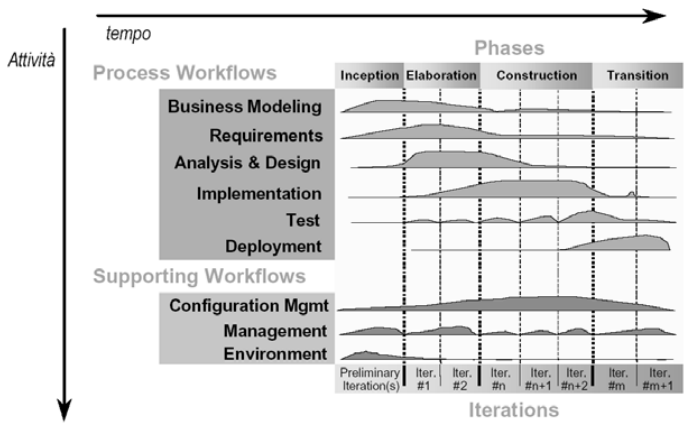
\includegraphics[width= \textwidth]{assets/fasiworkflow}
\end{center}

\section{Pianificazione iterazioni}
\label{sec:pianificazione_iterazioni}
Saranno di seguito elencate le iterazioni svolte durante il progetto, durante lo sviluppo compariranno le iterazioni già effettuate e la pianificazione dell'iterazione successiva.

\begin{center}
	\begin{tabularx}{\tabwidthiter}{ l  X } 
		\toprule
		\multicolumn{2}{c}{\tabtitleiter{Iterazione 01}}  \\
		\cmidrule(l{\cmidrulekern}r{\cmidrulekern}){1-2}
		\tabheaditer{Fase} & Inizio \\ 
		\addlinespace[1em] 
		\tabheaditer{Milestones} & 
		    \begin{enumWork}
			        \item Stesura del documento di richiesta
			        \item Stesura del documento di visione
			        \item Stesura dello studio di fattibilità
			        \item Stesura del contratto
			        \item Inizio stesura del glossario e degli acronimi
			        \item Inizio stesura del documento di pianificazione del progetto
		    \end{enumWork} \\
		\addlinespace[1em]
		\tabheaditer{Stato} &  Effettuata \\
		\bottomrule
	\end{tabularx}
\end{center}

\bigskip

\begin{center}
	\begin{tabularx}{\tabwidthiter}{ l  X } 
		\toprule
		\multicolumn{2}{c}{\tabtitleiter{Iterazione 02}}  \\
		\cmidrule(l{\cmidrulekern}r{\cmidrulekern}){1-2}
		\tabheaditer{Fase} & Elaborazione \\ 
		\addlinespace[1em] 
		\tabheaditer{Milestones} & 
		    \begin{enumWork}
			        \item Stesura del documento di specifica del sistema
			        \item Stesura del documento di specifica dei requisiti
			        \item Stesura del documento dei casi d'uso
			        \item Aggiornamento del glossario e degli acronimi
			        \item Aggiornamento del documento di pianificazione
		    \end{enumWork} \\
		\addlinespace[1em]
		\tabheaditer{Stato} &  In corso \\
		\bottomrule
	\end{tabularx}
\end{center}


\begin{landscape}
\section{Diagramma di Gantt}
\label{sec:diagramma_di_gantt}
Nel seguente diagramma di Gantt sono riportati i periodi di svolgimento di ogni attività effettuata per la realizzazione del sistema.

\begin{center}
	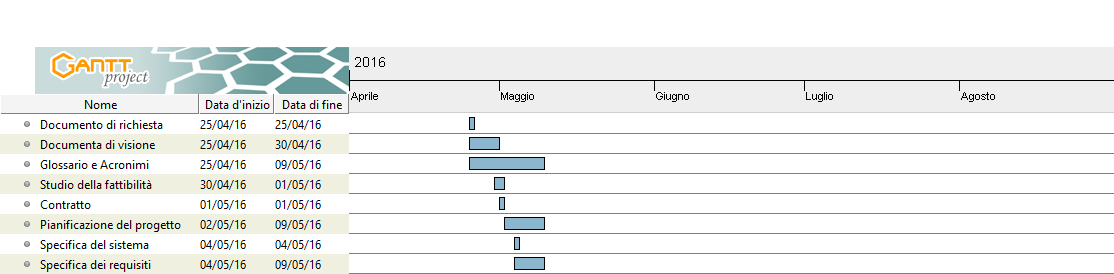
\includegraphics[width=\linewidth]{diagrammaGantt/DiagrammaGantt}
\end{center}
\end{landscape}

\newdate{pianuno}{3}{05}{2016}
\newdate{piandue}{4}{05}{2016}
\section{Revisioni}
\begin{center}
    \begin{tabular}{lll}
        \toprule
        \tabhead{Versione} & \tabhead{Data} & \tabhead{Descrizione} \\
        %   \cmidrule{2-3} 
        \midrule
        1.0 & \displaydate{pianuno} & Prima versione \\
        1.1 & \displaydate{piandue} & Aggiunta iterazione 02 \\
        \bottomrule
    \end{tabular}
\end{center}

    \chapter{Specifica sistema} 
\label{cha:specifica_sistema}

\section{Introduzione} 
In questo documento verrà descritto nel dettaglio il sistema nel suo complesso, in modo più approfondito rispetto al \docref{cha:documento_di_visione}.

\section{Descrizione dettagliata} 
\label{sec:descrizione_dettagliata}
Il portale che si vuole realizzare interagirà con diverse \grupporuolo{figure pubbliche}, che si distinguono tra autenticate e non autenticate. Fra le \grupporuolo{figure pubbliche autenticate} troviamo gli \ruolo{utenti} e i \ruolo{produttori}, mentre i \ruolo{visitatori} sono l'unica \grupporuolo{figura pubblica non autenticata}.
Sono presenti inoltre diverse \grupporuolo{figure amministrative}, quali i \ruolo{redattori}, gli \ruolo{assistenti} e i \ruolo{moderatori}.

\bigskip
\noindent
Le diverse figure presenti si distinguono a seconda di quali funzionalità, messe a disposizione dal sistema, possono utilizzare.

I \ruolo{visitatori} possono effettuare l'iscrizione, diversa a seconda della tipologia di account che si vuole creare, e l'autenticazione. Entrambe possono essere effettuate tramite l'integrazione con i principali Social Network, tuttavia per iscriversi come \ruolo{produttore} tramite Social Network si deve avere un account certificato in esso.

I \ruolo{produttori} hanno a disposizione uno spazio per pubblicizzare i loro prodotti, che da questo momento in avanti chiameremo \emph{vetrina}. Essi potranno dunque personalizzare la loro vetrina, inserendo informazioni e immagini sul \ruolo{produttore}, e possono inserire prodotti o modificare quelli già inseriti. L'inserimento di prodotti seguirà una rigida procedura per garantire la consistenza dei dati e facilitare la ricerca dei prodotti. Potranno inoltre commentare recensioni ai loro prodotti.

Gli \ruolo{utenti} possono valutare oppure effettuare una recensione, la quale aggiunge una descrizione testuale alla valutazione, dei prodotti. Una volta inserita una recensione o una valutazione è possibile modificarla, oppure è possibile eliminare la propria recensione. 
Per permettere di visualizzare velocemente le recensioni più utili, gli \ruolo{utenti} possono dare un giudizio positivo oppure negativo sulle recensioni presenti. Hanno inoltre la possibilità di commentare le recensioni, per permettere una maggiore interazione fra gli \ruolo{utenti}.
Per facilitare l'inserimento di informazioni nel portale sono state inoltre pensate due particolari funzionalità: l'\ruolo{utente} può suggerire un prodotto mancante ad un \ruolo{produttore} iscritto, e tale \ruolo{produttore} potrà scegliere se accettare o rifiutare la richiesta di inserimento, eventualmente modificando le informazioni inserite dall'\ruolo{utente}; inoltre l'\ruolo{utente} potrà suggerire al sistema un prodotto mancante di un \ruolo{produttore} esterno non ancora iscritto al portale. In questo caso il sistema raccoglierà le richieste indirizzate ad uno stesso \ruolo{produttore} e superata una certa soglia si valuterà la possibilità di contattare il \ruolo{produttore} per indurlo ad iscriversi nel portale (per il \ruolo{produttore} sarebbe vantaggioso, in quanto avrebbe molta pubblicità) oppure di creare la sua vetrina in sua vece.
Inoltre gli \ruolo{utenti} possono ricevere consigli sui prodotti che gli potrebbero piacere, tenendo conto dell'esperienza passata nel portale. 

\bigskip
\noindent
Alcune funzionalità sono comuni a diverse figure.

Le \grupporuolo{figure pubbliche autenticate} possono usufruire del sistema di follower/followed, possono quindi seguire altri account per ricevere aggiornamenti da essi, rimuovere account che si stanno seguendo oppure visualizzare gli aggiornamenti dagli account seguiti. Possono inoltre segnalare recensioni/commenti con contenuti non appropriati e aprire tickets per richiedere assistenza.

I \ruolo{visitatori} e gli \ruolo{utenti} possono ricevere consigli sui prodotti simili a quelli che si stanno visualizzando e notizie simili a quelle lette. 

Tutte le \grupporuolo{figure pubbliche} possono effettuare ricerche nel portale, in base a diversi criteri, di prodotti, di notizie e di profili pubblici.
Esse possono inoltre gestire il proprio account, con la possibilità di visualizzare il profilo (pubblico), accedere alle impostazioni (private), effettuare il logout oppure rimuovere l'account. Da notare che l'eventuale rimozione dell'account non comporterà la rimozione dei contenuti inseriti nel portale, ma solo la rimozione dello stesso. Possono inoltre visualizzare i contenuti pubblici del portale, quali le vetrine dei produttori, con eventuali statistiche, i singoli prodotti con le recensioni associate, i profili pubblici altrui con le statistiche associate a quell'account e le notizie presenti nel portale.

\bigskip
\noindent
Segue una descrizione delle funzionalità specifiche delle \grupporuolo{figure amministrative}, le quali oltre ad esse ereditano tutte le funzionalità specifiche degli \ruolo{utenti}.

I \ruolo{redattori} possono aggiungere, modificare o rimuovere notizie provenienti dal dolciario.

Gli \ruolo{assistenti} possono rispondere ai tickets per risolvere i problemi degli \ruolo{utenti}. Hanno inoltre il compito di gestire le iscrizioni dei produttori effettuate direttamente nel portale, controllando la veridicità delle informazioni inserite, ed in caso creare l'account richiesto.

I \ruolo{moderatori} che possono eliminare il contenuto non appropriato, che può essere segnalato tramite apposito ticket, dalle recensioni o dai commenti. Hanno la possibilità di eliminare completamente la recensione o il commento segnalato oppure di modificarle togliendo la parte incriminata. %VALENTINO SE LEGGI QUI DOBBIAMO DECIDERE!!!

\bigskip
\noindent
Nel portale che si vuole realizzare le informazioni sui prodotti sono di fondamentale importanza, perciò elenchiamo di seguito quelle contenute nel sistema:
\begin{itemize}
	\item \infoProdotto{Nome prodotto. }
	\item \infoProdotto{Almeno una foto dell’articolo.}
	\item \infoProdotto{Descrizione di presentazione.}
	\item \infoProdotto{Marca.}
	\item \infoProdotto{Categoria.}
	\item \infoProdotto{Particolarità.}
	\item \infoProdotto{Consistenza.}
	\item \infoProdotto{Ingredienti.}
	\item \infoProdotto{Altri campi} (a seconda di quali ha compilato il \ruolo{produttore}).
\end{itemize}
L'inserimento di queste informazioni è compito del \ruolo{produttore}, il quale seguirà una rigida procedura che sarà descritta nel dettaglio durante la specifica delle funzionalità.


\newdate{sisuno}{04}{05}{2016}
\section{Revisioni}
\begin{center}
    \begin{tabular}{lll}
        \toprule
        	\tabhead{Versione} & \tabhead{Data} & \tabhead{Descrizione} \\
		\cmidrule(l{\cmidrulekern}r{\cmidrulekern}){1-3}
        	1.0 & \displaydate{sisuno} & Prima versione \\
        \bottomrule
    \end{tabular}
\end{center}

    \chapter{Specifica requisiti} 
\label{cha:specifica_requisiti}

\section{Introduzione} 
In questo documento sono specificati nel dettaglio tutti i requisiti del sistema, suddivisi in funzionali e non funzionali.
Per organizzare in modo corretto le informazioni è stato adottato un sistema di codifica dei requisiti, descritto nella prossima sezione.

\section{Struttura del documento}
\label{sec:struttura_del_documento}

I requisiti mostrati sono prima elencati, per una più facile consultazione, e in seguito sono descritti in apposite tabelle. 
Ogni tabella contiene diverse informazioni:
\begin{itemize}
	\item Un \campiTabReq{id} per identificare univocamente il requisito.
	\item Un \campiTabReq{titolo} per semplificare il riconoscimento del requisito.
	\item Una \campiTabReq{descrizione} per indicare in cosa consiste la funzionalità rappresentata dal requisito.
	\item Un \campiTabReq{tipo} per indicare se il requisito è funzionale o non funzionale
	\item Una \campiTabReq{priorità} per indicare il grado di importanza del requisito.
	\item Lo \campiTabReq{stato} per indicare l'idoneità del requisito.
\end{itemize}

\subsection{Identificativo dei requisiti}
\label{subsec:identificativo_dei_requisiti}

Di seguito è spiegato come interpretare l'identificativo dei requisiti.
Un identificativo è della forma:
\begin{center}
	\subsubreq{tipo}{contesto}{categoria}{req}{[sottoreq]}{[\dots]}
\end{center}

\noindent
Segue una descrizione di ogni campo utilizzato nell'identificatore:
\begin{itemize}
	\item Il \campiIdReq{tipo} può essere:
	\begin{descriptionInd}
		\item[RF] indica un requisito funzionale.
		\item[RNF] indica un requisito non funzionale.
	\end{descriptionInd}

	\item Il \campiIdReq{contesto} serve ad identificare a quali figure è rivolta una data funzionalità, è un numero composto da 6 cifre ognuna delle quali può assumere un valore 0 oppure 1. La posizione della cifra si riferisce ad una specifica figura, se la cifra i-esima vale 1 significa che l'i-esima figura è presente nel contesto del requisitio, altrimenti no.
	Di seguito elenchiamo ogni posizione a quale figura riferisce: 
	\begin{descriptionInd}
		\item[1\textdegree\ bit] Visitatore.
		\item[2\textdegree\ bit] Utente.
		\item[3\textdegree\ bit] Produttore.
		\item[4\textdegree\ bit] Redattore.
		\item[5\textdegree\ bit] Assistente.
		\item[6\textdegree\ bit] Moderatore.
	\end{descriptionInd}		

	\item La \campiIdReq{categoria} è una lettera utilizzata per raggruppare i requisiti con scopi simili.
	Le categorie per i requisiti funzionali sono le seguenti:
	\begin{descriptionInd}
		\item[A] Iscrizione e autenticazione.
		\item[B] Gestione iscrizione.
		\item[C] Gestione vetrina.
		\item[D] Ricerca.
		\item[E] Gestione recensioni.
		\item[F] Gestione notizie.
		\item[G] Gestione follower/followed.
		\item[H] Gestioni suggerimenti.
		\item[I] Gestione account.
		\item[L] Visualizzazione contenuti.
	\end{descriptionInd}	
	Le categorie per i requisiti non funzionali sono le seguenti:
	\begin{descriptionInd}
		\item[A] Sicurezza.
		\item[B] Portabilità.
		\item[C] Usabilità.
		\item[D] Implementazione.
	\end{descriptionInd}	

	\item Il campo \campiIdReq{req} è un numero progressivo utilizzato per identificare in modo univoco un requisito all'interno della sua categoria.

	\item Il campo \campiIdReq{sottoreq} (opzionale) è un numero progressivo utilizzato per identificare in modo univoco un sotto--requisito di un dato requisito. Ci possono essere diversi campi sottoreq consecutivi, per esplicitare una nidificazione dei requisiti più dettagliata.
\end{itemize}

\subsection{Priorità}
\label{subsec:priorita}

La priorità di un requisito identifica quanto un requisito sia importante ai fini del completamento del sistema.
Qui di seguito sono elencati in breve i ``gradi di giudizio'' della priorità di un requisito:

\begin{descriptionInd}
	\item[Priorità Alta] Requisiti che il sistema deve necessariamente soddisfare.
	\item[Priorità Media] Requisiti la cui assenza non comporta grossi problemi per la soddisfacibilità del progetto: i requisiti base riescono comunque ad essere soddisfatti, con qualche sacrificio in termini di funzionalità. 
	\item[Priorità Bassa] Requisiti la cui assenza non comporta alcun tipo di problema per la soddisfacibilità del progetto. Questi requisiti possono anche visti come superflui o non strettamente necessari. La loro inclusione comporta un miglioramento della qualità complessiva dell’offerta dei servizi e delle funzionalità del progetto.
\end{descriptionInd}

\section{Elenco dei requisiti}
\label{sec:elenco_dei_requisiti}
Di seguito sono elencati tutti i requisiti, suddivisi in funzionali e non funzionali.

\subsection{Requisiti funzionali}
Vengono di seguito elencati i requisiti funzionali:
%USAGE: {keyrequisito}{\ereq{tipo}{contesto}{categoria}}{titolo} - doublelink automatico con \refDef{keyrequisito}
\begin{itemize} 
	\item \reqItem{req:iscrizione}{\ereq{RF}{100000}{A}}{Iscrizione}
	\item \reqItem{req:iscrizionePortale}{\esubreq{RF}{100000}{A}}{Iscrizione tramite modulo del portale}
	\item \reqItem{req:iscrizioneSocial}{\esubreq{RF}{100000}{A}}{Iscrizione tramite Social Network}
	\item \reqItem{req:iscrizioneSocialVer}{\esubsubreq{RF}{100000}{A}}{Iscrizione tramite Social Network verificati}
	\item \reqItem{req:iscrizioneSocialNotVer}{\esubsubreq{RF}{100000}{A}}{Iscrizione tramite Social Network non verificati}
	\item \reqItem{req:iscrizioneApprovazione}{\esubreq{RF}{100000}{A}}{Iscrizione tramite approvazione}
	
	\item \reqItem{req:login}{\ereq{RF}{100000}{A}}{Login}
	\countReset 
	
	\item \reqItem{req:approvazioneIscrizione}{\ereq{RF}{000010}{B}}{Approvazione iscrizione}
	
	\item \reqItem{req:rimozioneAccountAltrui}{\ereq{RF}{000001}{B}}{Rimozione account altrui}
	\countReset
	
	\item \reqItem{req:personalizzaVetrina}{\ereq{RF}{001000}{C}}{Personalizzione vetrina}
	\item \reqItem{req:personalizzaVetrinaInsDesc}{\esubreq{RF}{001000}{C}}{Inserimento descrizione}
	\item \reqItem{req:personalizzaVetrinaInsImg}{\esubreq{RF}{001000}{C}}{Inserimento immagine}
	\item \reqItem{req:personalizzaVetrinaInsProd}{\esubreq{RF}{001000}{C}}{Inserimento prodotto}
	\item \reqItem{req:personalizzaVetrinaModProd}{\esubreq{RF}{001000}{C}}{Modifica prodotto}
	
	\item \reqItem{req:statistichePrivateVetrina}{\ereq{RF}{001000}{C}}{Visualizzazione statistiche private della vetrina}
	\countReset
	
	\item \reqItem{req:ricercaInfo}{\ereq{RF}{111111}{D}}{Ricerca informazioni}
	\item \reqItem{req:ricercaProdotto}{\esubreq{RF}{111111}{D}}{Ricerca prodotto}
	\item \reqItem{req:ricercaProfilo}{\esubreq{RF}{111111}{D}}{Ricerca profilo}
	\item \reqItem{req:ricercaNotizia}{\esubreq{RF}{111111}{D}}{Ricerca notizia}

	\item \reqItem{req:richiestaInsProdotto}{\ereq{RF}{010000}{D}}{Richiesta inserimento prodotto a un produttore iscritto}

	\item \reqItem{req:richiestaInsProduttore}{\ereq{RF}{010000}{D}}{Richiesta inserimento prodotto e del suo produttore}
	\countReset

	\item \reqItem{req:valutazioneProdotto}{\ereq{RF}{010111}{E}}{Valutazione prodotto}
	\item \reqItem{req:inserisciValutazioneProdotto}{\esubreq{RF}{010111}{E}}{Inserimento valutazione}
	\item \reqItem{req:modificaValutazioneProdotto}{\esubreq{RF}{010111}{E}}{Modifica valutazione inserita}
	\item \reqItem{req:eliminaValutazioneProdotto}{\esubreq{RF}{010111}{E}}{Rimozione valutazione inserita}

	\item \reqItem{req:recensioneProdotto}{\ereq{RF}{010111}{E}}{Recensione prodotto}
	\item \reqItem{req:inserisciRecensioneProdotto}{\esubreq{RF}{010111}{E}}{Inserimento recensione}
	\item \reqItem{req:modificaRecensioneProdotto}{\esubreq{RF}{010111}{E}}{Modifica valutazione inserita}
	\item \reqItem{req:eliminaRecensioneProdotto}{\esubreq{RF}{010111}{E}}{Rimozione recensione inserita}

	\item \reqItem{req:commentoRecensione}{\ereq{RF}{011111}{E}}{Commento a recensione}
	
	\item \reqItem{req:valutaRecensione}{\ereq{RF}{010111}{E}}{Valutazione recensione}
	
	\item \reqItem{req:segnalazioneContenuti}{\ereq{RF}{011111}{E}}{Segnalazione contenuti inappropriati}
	
	\item \reqItem{req:rimozioneRecensioneInap}{\ereq{RF}{000001}{E}}{Rimozione recensione inappropriata}
	\countReset

	\item \reqItem{req:inserimentoNotizia}{\ereq{RF}{000100}{F}}{Inserimento notizia}
	
	\item \reqItem{req:modificaNotizia}{\ereq{RF}{000100}{F}}{Modifica notizia}
	
	\item \reqItem{req:rimozioneNotizia}{\ereq{RF}{000100}{F}}{Rimozione notizia}
	\countReset
	
	\item \reqItem{req:followAccount}{\ereq{RF}{011111}{G}}{Follow account}
	
	\item \reqItem{req:unFollowAccount}{\ereq{RF}{011111}{G}}{Unfollow account}
	\countReset

	\item \reqItem{req:suggerimentoProdotti}{\ereq{RF}{011111}{H}}{Suggerimento prodotti intelligente}
	
	\item \reqItem{req:prodottiSimili}{\ereq{RF}{011111}{H}}{Suggerimento prodotti simili}

	\item \reqItem{req:notizieSimili}{\ereq{RF}{011111}{H}}{Suggerimento notizie simili}
	\countReset

	\item \reqItem{req:accessoProfilo}{\ereq{RF}{011111}{I}}{Accesso al proprio profilo}
	
	\item \reqItem{req:accessoImpostazioni}{\ereq{RF}{011111}{I}}{Accesso alle proprie impostazioni}

	\item \reqItem{req:rimozioneAccountProprio}{\ereq{RF}{011111}{I}}{Rimozione account proprio}
	
	\item \reqItem{req:logout}{\ereq{RF}{011111}{I}}{Logout}
	\countReset
	
	\item \reqItem{req:visualizzazioneVetrina}{\ereq{RF}{111111}{L}}{Visualizzazione vetrina}
	\item \reqItem{req:visualizzazioneStatistichePubVetrina}{\esubreq{RF}{111111}{L}}{Visualizzazione statische pubbliche vetrina}
	\item \reqItem{req:visualizzazioneProdottiVetrina}{\esubreq{RF}{111111}{L}}{Visualizzazione prodotti esposti in vetrina}

	\item \reqItem{req:visualizzazioneProdotto}{\ereq{RF}{111111}{L}}{Visualizzazione prodotto}
	\item \reqItem{req:visualizzazioneInfoProdotto}{\esubreq{RF}{111111}{L}}{Visualizzazione informazioni del prodotto}
	\item \reqItem{req:visualizzazioneRecProdotto}{\esubreq{RF}{111111}{L}}{Visualizzazione recensioni associate al prodotto}
	\item \reqItem{req:visualizzazioneStatProdotto}{\esubreq{RF}{111111}{L}}{Visualizzazione statistiche del prodotto}

	\item \reqItem{req:visualizzazioneProfilo}{\ereq{RF}{111111}{L}}{Visualizzazione profilo pubblico}
	\item \reqItem{req:visualizzazioneInfoProfilo}{\esubreq{RF}{111111}{L}}{Visualizzazione informazioni di un profilo pubblico}
	\item \reqItem{req:visualizzazioneStatProfilo}{\esubreq{RF}{111111}{L}}{Visualizzazione statistiche di un profilo pubblico}

	\item \reqItem{req:visualizzazioneNotizie}{\ereq{RF}{111111}{L}}{Visualizzazione notizie}
	
	\item \reqItem{req:visualizzazioneAggF}{\ereq{RF}{011111}{L}}{Visualizzazione aggiornamenti dai followed}
\end{itemize}	


\subsection{Requisiti non funzionali}
\label{sub:requisiti_non_funzionali}


\section{Descrizione dei requisiti}
\label{sec:descrizione_dei_requisiti}
Di seguito sono presenti tutte le descrizioni dei requisiti, suddivise in funzionali e non funzionali.

\subsection{Requisiti funzionali}
Vengono di seguito riportate le tabelle che descrivono nel dettaglio ogni requisito funzionale.

\reqTabRF{req:iscrizione}{}{}{}

\tabreqvspace

\reqTabRF{req:iscrizionePortale}{}{}{}

\tabreqvspace

\reqTabRF{req:iscrizioneSocial}{}{}{}

\tabreqvspace

\reqTabRF{req:iscrizioneSocialVer}{}{}{}

\tabreqvspace

\reqTabRF{req:iscrizioneSocialNotVer}{}{}{}

\tabreqvspace

\reqTabRF{req:iscrizioneApprovazione}{}{}{}

\tabreqvspace

\reqTabRF{req:login}{}{}{}

\tabreqvspace

\reqTabRF{req:approvazioneIscrizione}{}{}{}

\tabreqvspace

\reqTabRF{req:rimozioneAccountAltrui}{}{}{}

\tabreqvspace

\reqTabRF{req:personalizzaVetrina}{}{}{}

\tabreqvspace

\reqTabRF{req:personalizzaVetrinaInsDesc}{}{}{}

\tabreqvspace

\reqTabRF{req:personalizzaVetrinaInsImg}{}{}{}

\tabreqvspace

\reqTabRF{req:personalizzaVetrinaInsProd}{}{}{}

\tabreqvspace

\reqTabRF{req:personalizzaVetrinaModProd}{}{}{}

\tabreqvspace

\reqTabRF{req:statistichePrivateVetrina}{}{}{}

\tabreqvspace

\reqTabRF{req:ricercaInfo}{}{}{}

\tabreqvspace

\reqTabRF{req:ricercaProdotto}{}{}{}

\tabreqvspace

\reqTabRF{req:ricercaProfilo}{}{}{}

\tabreqvspace

\reqTabRF{req:ricercaNotizia}{}{}{}

\tabreqvspace

\reqTabRF{req:richiestaInsProdotto}{}{}{}

\tabreqvspace

\reqTabRF{req:richiestaInsProduttore}{}{}{}

\tabreqvspace

\reqTabRF{req:valutazioneProdotto}{}{}{}

\tabreqvspace

\reqTabRF{req:inserisciValutazioneProdotto}{}{}{}

\tabreqvspace

\reqTabRF{req:modificaValutazioneProdotto}{}{}{}

\tabreqvspace

\reqTabRF{req:eliminaValutazioneProdotto}{}{}{}

\tabreqvspace

\reqTabRF{req:recensioneProdotto}{}{}{}

\tabreqvspace

\reqTabRF{req:inserisciRecensioneProdotto}{}{}{}

\tabreqvspace

\reqTabRF{req:modificaRecensioneProdotto}{}{}{}

\tabreqvspace

\reqTabRF{req:eliminaRecensioneProdotto}{}{}{}

\tabreqvspace

\reqTabRF{req:commentoRecensione}{}{}{}

\tabreqvspace

\reqTabRF{req:valutaRecensione}{}{}{}

\tabreqvspace

\reqTabRF{req:segnalazioneContenuti}{}{}{}

\tabreqvspace

\reqTabRF{req:rimozioneRecensioneInap}{}{}{}

\tabreqvspace

\reqTabRF{req:inserimentoNotizia}{}{}{}

\tabreqvspace

\reqTabRF{req:modificaNotizia}{}{}{}

\tabreqvspace

\reqTabRF{req:rimozioneNotizia}{}{}{}

\tabreqvspace

\reqTabRF{req:followAccount}{}{}{}

\tabreqvspace

\reqTabRF{req:unFollowAccount}{}{}{}

\tabreqvspace

\reqTabRF{req:suggerimentoProdotti}{}{}{}

\tabreqvspace

\reqTabRF{req:prodottiSimili}{}{}{}

\tabreqvspace

\reqTabRF{req:notizieSimili}{}{}{}

\tabreqvspace

\reqTabRF{req:accessoProfilo}{}{}{}

\tabreqvspace

\reqTabRF{req:accessoImpostazioni}{}{}{}

\tabreqvspace

\reqTabRF{req:rimozioneAccountProprio}{}{}{}

\tabreqvspace

\reqTabRF{req:logout}{}{}{}

\tabreqvspace

\reqTabRF{req:visualizzazioneVetrina}{}{}{}

\tabreqvspace

\reqTabRF{req:visualizzazioneStatistichePubVetrina}{}{}{}

\tabreqvspace

\reqTabRF{req:visualizzazioneProdottiVetrina}{}{}{}

\tabreqvspace

\reqTabRF{req:visualizzazioneProdotto}{}{}{}

\tabreqvspace

\reqTabRF{req:visualizzazioneInfoProdotto}{}{}{}

\tabreqvspace

\reqTabRF{req:visualizzazioneRecProdotto}{}{}{}

\tabreqvspace

\reqTabRF{req:visualizzazioneStatProdotto}{}{}{}

\tabreqvspace

\reqTabRF{req:visualizzazioneProfilo}{}{}{}

\tabreqvspace

\reqTabRF{req:visualizzazioneInfoProfilo}{}{}{}

\tabreqvspace

\reqTabRF{req:visualizzazioneStatProfilo}{}{}{}

\tabreqvspace

\reqTabRF{req:visualizzazioneNotizie}{}{}{}

\tabreqvspace

\reqTabRF{req:visualizzazioneAggF}{}{}{}

\subsection{Requisiti non funzionali}
Vengono di seguito riportate le tabelle che descrivono nel dettaglio ogni requisito non funzionale.
    \chapter{Specifica dei casi d'uso}

\section{Introduzione}
In questo documento sono analizzati ed elencati gli attori ed i casi d'uso del sistema.
Scopo del documento è la dettagliata descrizione delle modalità di interazione tra le diverse entità presenti ed il sistema.
Ciò permetterà di mettere in evidenza eventuali conflitti tra i requisiti del sistema stesso.
Tale analisi e descrizione dei casi d'uso verrà presentata tramite grafici che seguono lo standard UML.

\noindent
Si utilizzeranno le seguenti convenzioni:
\begin{itemize}
	\item Nei casi in cui più attori possono accedere ad un determinato caso d’uso, ma quest'ultimo è rivolto principalmente ad un solo attore, non verranno elencati tutti gli altri.

	\item Non verranno riportati tutti gli attori che hanno accesso ad un determinato caso d'uso, ma solo l'attore più generico.
	
	\item Nei diagrammi dei casi d'uso non viene riportato l'identificatore del singolo caso d'uso ma solo il titolo, per facilitarne la lettura.

	\item Nella descrizione dei flussi dei casi d'uso, si assume che sia sempre possibile tornare al passo precedente che richiede interazione con la persona, ad eccezione dei passi in cui si è data una conferma.

	\item Nella descrizione dei flussi alternativi dei casi d'uso, quando si indica la modifica di alcuni punti e non si nominano gli altri, si assume che gli altri rimangano immutati.
\end{itemize}

\section{Elenco degli attori}
Gli attori che interagiscono con il portale sono elencati di seguito:
\begin{itemize}
	\item \newListItem{att:visitatore}{\formattaAtt}{Visitatore}
	\item \newListItem{att:figuraPubblicaAutenticata}{\formattaAtt}{Figura Pubblica Autenticata}
	\item \newListItem{att:figuraAmministrativa}{\formattaAtt}{Figura Amministrativa}
	\item \newListItem{att:utente}{\formattaAtt}{Utente}
	\item \newListItem{att:produttore}{\formattaAtt}{Produttore}
	\item \newListItem{att:redattore}{\formattaAtt}{Redattore}
	\item \newListItem{att:assistente}{\formattaAtt}{Assistente}
	\item \newListItem{att:moderatore}{\formattaAtt}{Moderatore}
	\item \newListItem{att:amministratore}{\formattaAtt}{Amministratore}
	\item \newListItem{att:cms}{\formattaAtt}{CMS}
\end{itemize}
La gerarchia degli attori è mostrata nel seguente diagramma UML:
\begin{center}
   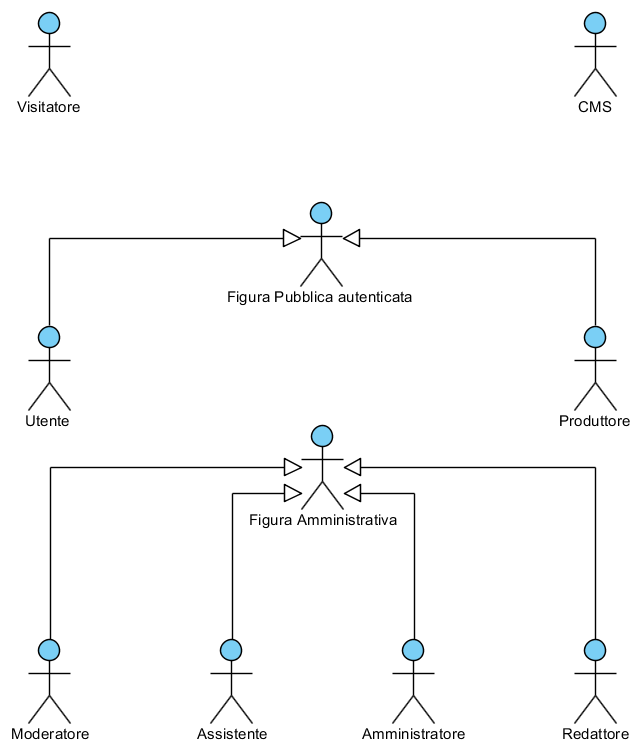
\includegraphics[width=\textwidth]{assets/visualParadigm/cu/SchemaAttori}
\end{center}

\section{Specifica degli attori}
Gli attori che interagiscono con il portale sono descritti di seguito:
\attTab{att:visitatore}{-}{\glsdesc*{visitatore}}

\vspaceTab

\attTab{att:figuraPubblicaAutenticata}{-}{\glsdesc*{figuraPubblicaAutenticata}}

\vspaceTab

\attTab{att:figuraAmministrativa}{-}{\glsdesc*{figuraAmministrativa}}

\vspaceTab

\attTab{att:utente}{\getTitletodesc{att:figuraPubblicaAutenticata}}{\glsdesc*{utente}}

\vspaceTab

\attTab{att:produttore}{\getTitletodesc{att:figuraPubblicaAutenticata}}{\glsdesc*{produttore}}

\vspaceTab

\attTab{att:redattore}{\getTitletodesc{att:figuraAmministrativa}}{\glsdesc*{redattore}}

\vspaceTab

\attTab{att:assistente}{\getTitletodesc{att:figuraAmministrativa}}{\glsdesc*{assistente}}

\vspaceTab

\attTab{att:moderatore}{\getTitletodesc{att:figuraAmministrativa}}{\glsdesc*{moderatore}}

\vspaceTab

\attTab{att:amministratore}{\getTitletodesc{att:figuraAmministrativa}}{\glsdesc*{amministratore}}

\vspaceTab

\attTab{att:cms}{-}{\glsdesc*{cmsdef}}

\section{Identificativo dei casi d'uso} %(vengono usati per definire l'ID, non ha senso metterli dopo la struttura ID)
Di seguito è spiegato come interpretare l'identificativo dei casi d'uso:
\begin{center}
	\use{categoria}{caso}%{[sottoreq]}{[\dots]}
\end{center}

\noindent
Segue una descrizione di ogni campo utilizzato nell'identificatore:
\begin{itemize}
	\item La \campiIdReq{categoria} è una lettera utilizzata per raggruppare i casi d'uso con scopi simili.
	Le categorie sono le seguenti:
	\begin{enumerateIndLabel}{\textsf{\Alph*}}{\Alph*}
		\item Autenticazione. \label{pkg:autenticazione}
		\item Gestione iscrizioni. \label{pkg:iscrizione}
		\item Gestione vetrina. \label{pkg:vetrina} 
		\item Gestione notizie. \label{pkg:notizie}
		\item Gestione suggerimenti. \label{pkg:suggerimenti}
		\item Gestione account. \label{pkg:account}
		\item Gestione valutazioni. \label{pkg:gestionevalutazione}
		\item Gestione recensioni. \label{pkg:gestionerecensione}
		\item Interazione tra figure. \label{pkg:interazione}
		\item Gestione ticket. \label{pkg:gestioneticket}
		\item Ricerca contenuti. \label{pkg:ricerca}
		\item Gestione prodotti mancanti. \label{pkg:prodottimancanti}
		\item Visualizzazione contenuti pubblici. \label{pkg:visualizzazione}
	\end{enumerateIndLabel}

	\item Il campo \campiIdReq{caso} è un numero progressivo utilizzato per identificare in modo univoco un caso d'uso all'interno della sua categoria.
\end{itemize}

\section{Elenco dei casi d'uso}
Vengono di seguito elencati i casi d'uso:
\begin{itemize} 
	\setCatCU{\ref*{pkg:autenticazione}}%A
	\item \newListItem{cu:login}{\formattaCU}{Login}
	\item \newListItem{cu:loginAmm}{\formattaCU}{Login Figure Amministrative}
	\item \newListItem{cu:logout}{\formattaCU}{Logout}

	\setCatCU{\ref*{pkg:iscrizione}}%B
	\item \newListItem{cu:iscrizionePortale}{\formattaCU}{Iscrizione tramite modulo}
	\item \newListItem{cu:iscrizioneSocial}{\formattaCU}{Iscrizione tramite Social Network}
	\item \newListItem{cu:iscrizioneApprovazione}{\formattaCU}{Iscrizione tramite approvazione}
	\item \newListItem{cu:approvazioneIscrizione}{\formattaCU}{Approvazione iscrizione}

	\setCatCU{\ref*{pkg:vetrina}}%C
	\item \newListItem{cu:personalizzaVetrinaInsDesc}{\formattaCU}{Inserimento descrizione}
	\item \newListItem{cu:personalizzaVetrinaModDesc}{\formattaCU}{Modifica descrizione}
	\item \newListItem{cu:personalizzaVetrinaInsImg}{\formattaCU}{Inserimento immagine}
	\item \newListItem{cu:personalizzaVetrinaDelImg}{\formattaCU}{Rimozione immagine}
	\item \newListItem{cu:personalizzaVetrinaInsProd}{\formattaCU}{Inserimento scheda prodotto}
	\item \newListItem{cu:personalizzaVetrinaModProd}{\formattaCU}{Modifica scheda prodotto}
	\item \newListItem{cu:statistichePrivateVetrina}{\formattaCU}{Mostra statistiche private della vetrina}


	\setCatCU{\ref*{pkg:notizie}}%D
	\item \newListItem{cu:inserimentoNotizia}{\formattaCU}{Inserimento notizia}
	\item \newListItem{cu:modificaNotizia}{\formattaCU}{Modifica notizia}
	\item \newListItem{cu:rimozioneNotizia}{\formattaCU}{Rimozione notizia}

	\setCatCU{\ref*{pkg:suggerimenti}}%E
	\item \newListItem{cu:suggerimentoProdotti}{\formattaCU}{Suggerimento prodotti}
	\item \newListItem{cu:notizieSimili}{\formattaCU}{Suggerimento notizie}
	
	\setCatCU{\ref*{pkg:account}}%F
	\item \newListItem{cu:modificaProfilo}{\formattaCU}{Modifica del proprio profilo}
	\item \newListItem{cu:inserisciImgProfilo}{\formattaCU}{Inserimento immagine profilo proprio}
	\item \newListItem{cu:rimuoviImgProfilo}{\formattaCU}{Rimozione immagine profilo proprio}
	\item \newListItem{cu:modificaImpostazioni}{\formattaCU}{Modifica delle proprie impostazioni}
	\item \newListItem{cu:rimozioneAccountProprio}{\formattaCU}{Rimozione account proprio}
	\item \newListItem{cu:rimozioneAccountAltrui}{\formattaCU}{Rimozione account altrui}
	\item \newListItem{cu:modificaPrivilegiAccount}{\formattaCU}{Modifica privilegi di un account}


	\setCatCU{\ref*{pkg:gestionevalutazione}}%G
	\item \newListItem{cu:inserisciValutazioneProdotto}{\formattaCU}{Inserimento valutazione}
	\item \newListItem{cu:modificaValutazioneProdotto}{\formattaCU}{Modifica valutazione}

	\setCatCU{\ref*{pkg:gestionerecensione}}%H
	\item \newListItem{cu:inserisciRecensioneProdotto}{\formattaCU}{Inserimento recensione}
	\item \newListItem{cu:modificaRecensioneProdotto}{\formattaCU}{Modifica recensione propria}
	\item \newListItem{cu:eliminaRecensioneProdotto}{\formattaCU}{Rimozione recensione propria}
	\item \newListItem{cu:commentoRecensione}{\formattaCU}{Commento a recensione}
	\item \newListItem{cu:giudizioRecensione}{\formattaCU}{Giudizio recensione}
	\item \newListItem{cu:modificaGiudizioRecensione}{\formattaCU}{Modifica giudizio recensione}
	\item \newListItem{cu:segnalazioneContenutiInap}{\formattaCU}{Segnalazione contenuti inappropriati}
	\item \newListItem{cu:mostraSegnContenutiInap}{\formattaCU}{Mostra segnalazioni contenuti}
	\item \newListItem{cu:rimozioneContenutiInap}{\formattaCU}{Rimozione contenuti inappropriati}

	\setCatCU{\ref*{pkg:interazione}}%I
	\item \newListItem{cu:followAccount}{\formattaCU}{Follow account}
	\item \newListItem{cu:unFollowAccount}{\formattaCU}{Unfollow account}

	\setCatCU{\ref*{pkg:gestioneticket}}%J
	\item \newListItem{cu:ticketInvio}{\formattaCU}{Invio di un ticket}
	\item \newListItem{cu:ticketRisposta}{\formattaCU}{Risposta ad un ticket}
	\item \newListItem{cu:ticketChiudi}{\formattaCU}{Chiusura di un ticket}
	\item \newListItem{cu:ticketLettura}{\formattaCU}{Lettura di un ticket}

	\setCatCU{\ref*{pkg:ricerca}}%K
	\item \newListItem{cu:ricercaProdotto}{\formattaCU}{Ricerca prodotto}
	\item \newListItem{cu:ricercaProfilo}{\formattaCU}{Ricerca profilo}
	\item \newListItem{cu:ricercaNotizia}{\formattaCU}{Ricerca notizia}

	\setCatCU{\ref*{pkg:prodottimancanti}}%L
	\item \newListItem{cu:richiestaInsProdotto}{\formattaCU}{Richiesta inserimento scheda prodotto}
	\item \newListItem{cu:mostraRichiestaInsProdotto}{\formattaCU}{Mostra richiesta scheda prodotto}
	\item \newListItem{cu:richiestaInsProduttore}{\formattaCU}{Richiesta inserimento produttore e scheda prodotto}

	\setCatCU{\ref*{pkg:visualizzazione}}%M
	\item \newListItem{cu:mostraVetrina}{\formattaCU}{Mostra vetrina}
	\item \newListItem{cu:mostraProdotto}{\formattaCU}{Mostra scheda prodotto}
	\item \newListItem{cu:mostraRecensioniProdotto}{\formattaCU}{Mostra recensioni associate al prodotto}
	\item \newListItem{cu:mostraRecensione}{\formattaCU}{Mostra recensione}
	\item \newListItem{cu:mostraProfilo}{\formattaCU}{Mostra profilo pubblico}
	\item \newListItem{cu:mostraNotizia}{\formattaCU}{Mostra notizia}
	\item \newListItem{cu:mostraAggF}{\formattaCU}{Mostra aggiornamenti dai followed}
\end{itemize}	

%{id}{attori}{pre}{post}{flusso}
\section{Specifica dei casi d'uso}
Vengono di seguito elencate le tabelle che descrivono i casi d'uso, suddivisi per categoria:

\subsection{Autenticazione}
\begin{center}
   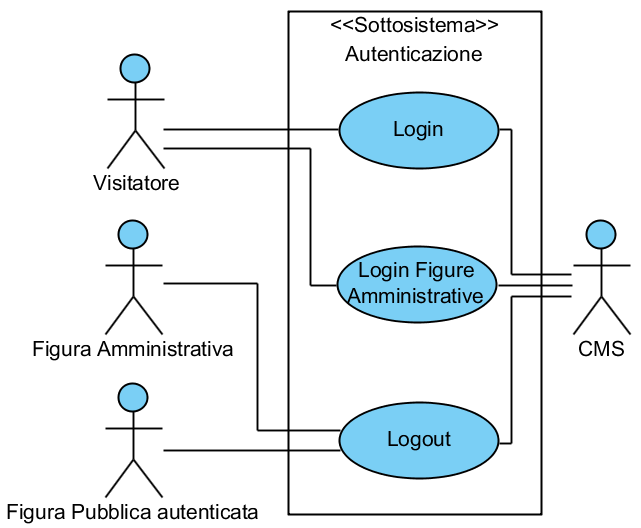
\includegraphics[width=\textwidth]{assets/visualParadigm/cu/Autenticazione}
\end{center}
%*************** LOGIN *****************
\cuTab{cu:login}%
{\getTitletodesc{att:visitatore}}%
{La persona connessa al sito è inizialmente riconosciuta come Visitatore}%
{La persona connessa al sito è ora riconosciuta come Figura Pubblica Autenticata}%
{\begin{enumCU}
	\item Il caso d'uso ha inizio quando un Visitatore richiede di effettuare il login 
	\item Il sistema richiede le credenziali di autenticazione
	\item Il Visitatore inserisce le credenziali di accesso negli appositi campi \label{culogin:3}
	\item Il Visitatore conferma i dati inseriti
	\item Il sistema verifica che i dati inseriti corrispondano ad un account pubblico esistente\label{culogin:5}
	\item Il sistema accetta le credenziali ricevute
\end{enumCU}}%
%
\cuAlternativo{cu:login}
{Flusso alternativo 1}%
{Errore Login}%
{La persona connessa al sito è inizialmente riconosciuta come Visitatore}%
{\postNulle}%
{\begin{enumCU}
	\item Dopo il punto \ref{culogin:5} il sistema rifiuta le credenziali
\end{enumCU}}%
%
\cuAlternativo{cu:login}
{Flusso alternativo 2}%
{Annulla Login}%
{La persona connessa al sito è inizialmente riconosciuta come Visitatore}%
{\postNulle}%
{\begin{enumCU}
		\item Dopo il punto \ref{culogin:3} il Visitatore annulla l'operazione di login
\end{enumCU}}%

\vspaceTab

\cuTab{cu:loginAmm}%
{\getTitletodesc{att:visitatore}}%
{La persona connessa al sito è inizialmente riconosciuta come Visitatore}%
{La persona connessa al sito è ora riconosciuta come Figura Amministrativa}%
{\begin{enumCU}
	\item Il caso d'uso ha inizio quando un Visitatore richiede di effettuare il login 
	\item Il sistema richiede le credenziali di autenticazione
	\item Il Visitatore inserisce le credenziali di accesso negli appositi campi \label{culoginamm:3}
	\item Il Visitatore conferma i dati inseriti
	\item Il sistema verifica che i dati inseriti corrispondano ad un account amministrativo esistente\label{culoginamm:5}
	\item Il sistema accetta le credenziali ricevute
	\item Il sistema invia un codice casuale sul cellulare del Visitatore
	\item Il Visitatore inserisce il codice ricevuto sul cellulare in un apposito campo \label{culoginamm:8}
	\item Il Visitatore conferma il codice inserito
	\item Il sistema verifica che il codice inserito corrisponda a quello inviato \label{culoginamm:10}
	\item Il sistema accetta il codice ricevuto
\end{enumCU}}%
%
\cuAlternativo{cu:loginAmm}
{Flusso alternativo 1}%
{Errore Credenziali}%
{La persona connessa al sito è inizialmente riconosciuta come Visitatore}%
{\postNulle}%
{\begin{enumCU}
	\item Dopo il punto \ref{culoginamm:5} il sistema rifiuta le credenziali
\end{enumCU}}%
%
\cuAlternativo{cu:loginAmm}
{Flusso alternativo 2}%
{Annulla Credenziali}%
{La persona connessa al sito è inizialmente riconosciuta come Visitatore}%
{\postNulle}%
{\begin{enumCU}
		\item Dopo il punto \ref{culoginamm:3} il Visitatore annulla l'operazione di login
\end{enumCU}}%
%
\cuAlternativo{cu:loginAmm}
{Flusso alternativo 3}%
{Errore Codice}%
{La persona connessa al sito è inizialmente riconosciuta come Visitatore}%
{\postNulle}%
{\begin{enumCU}
		\item Dopo il punto \ref{culoginamm:10}, il sistema rifiuta il codice
\end{enumCU}}%
%
\cuAlternativo{cu:loginAmm}
{Flusso alternativo 4}%
{Annulla Codice}%
{La persona connessa al sito è inizialmente riconosciuta come Visitatore}%
{\postNulle}%
{\begin{enumCU}
		\item Dopo il punto \ref{culoginamm:8}, il Visitatore annulla l'operazione di login
\end{enumCU}}%

\vspaceTab

%*************** LOGOUT *****************
\cuTab{cu:logout}
{\getTitletodesc{att:figuraAmministrativa}, \getTitletodesc{att:figuraPubblicaAutenticata}}
{La persona connessa al sito è autenticata}
{La persona connessa al sito non è più autenticata ed è ora un Visitatore}
{\begin{enumCU}
	\item Il caso d'uso ha inizio quando una persona autenticata richiede di effettuare il logout
	\item Il sistema effettua il logout richiesto
\end{enumCU}}

\subsection{Gestione iscrizioni}
\begin{center}
   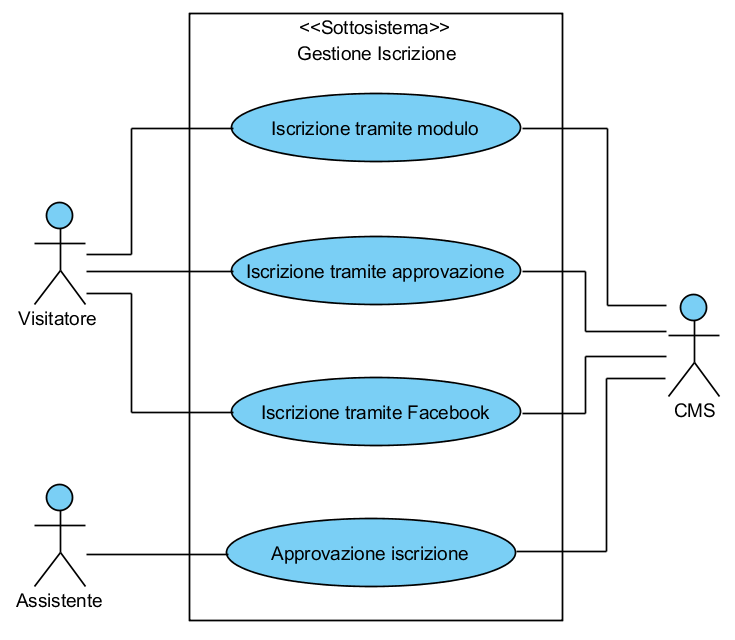
\includegraphics[width=\textwidth]{assets/visualParadigm/cu/GestioneIscrizione}
\end{center}
%*************** ISCRIZIONE PORTALE *****************
\cuTab{cu:iscrizionePortale}
{\getTitletodesc{att:visitatore}}
{La persona connessa al sito è inizialmente riconosciuta come Visitatore}
{La persona ha ora un account proprio, creato con i dati da essa inseriti}
{\begin{enumCU}
	\item Il caso d'uso ha inizio quando un Visitatore richiede di effettuare l'iscrizione
	\item Il sistema richiede i dati richiesti per effettuare l'iscrizione tra cui un identificatore all'interno del sistema
	\item Il Visitatore inserisce i dati richiesti negli appositi campi \label{cuiscr:3}
	\item Il Visitatore conferma i dati inseriti
	\item Il sistema verifica che i dati inseriti siano corretti e che l'identificatore dell'account che si sta creando non sia già presente \label{cuiscr:5}
	\item Il sistema crea un nuovo account con le credenziali ricevute
\end{enumCU}}
%
\cuAlternativo{cu:iscrizionePortale}
{Flusso alternativo 1}%
{Annulla iscrizione}%
{La persona connessa al sito è inizialmente riconosciuta come Visitatore}%
{\postNulle}%
{\begin{enumCU}
		\item Dopo il punto \ref{cuiscr:3} l'utente annulla l'operazione di iscrizione
	\end{enumCU}}%
%
\cuAlternativo{cu:iscrizionePortale}
{Flusso alternativo 2}%
{Errore iscrizione}%
{La persona connessa al sito è inizialmente riconosciuta come Visitatore}%
{\postNulle}%
{\begin{enumCU}
		\item Dopo il punto \ref{cuiscr:5} il sistema rileva un errore nei dati inseriti
	\end{enumCU}}%


\vspaceTab

%%%FORSE DA TOGLIERE -------------------------------------------------------------------------
%Accorpa verificati e non verificati
\cuTab{cu:iscrizioneSocial}
{\getTitletodesc{att:visitatore}}
{La persona è connessa al sito come Visitatore}
{La persona ha ora un account proprio, creato tramite le API messe a disposizione dal Social Network utilizzato durante l'iscrizione}
{\begin{enumCU}
		\item Il caso d'uso ha inizio quando un Visitatore richiede di effettuare l'iscrizione tramite un Social Network
		\item Il sistema richiede le credenziali di accesso del Social Network scelto
		\item Il Visitatore inserisce i dati richiesti \label{cuiscrappsocial:3}
		\item Il Visitatore conferma i dati inseriti \label{cuiscrappsocial:5}
		\item Il Il sistema crea un nuovo account con le credenziali ricevute
	\end{enumCU}}

\vspaceTab
%
\cuAlternativo{cu:iscrizioneSocial}
{Flusso alternativo 1}%
{Annulla iscrizione}%
{La persona connessa al sito è inizialmente riconosciuta come Visitatore}%
{\postNulle}%
{\begin{enumCU}
		\item Dopo il punto \ref{cuiscrappsocial:3} il Visitatore annulla l'operazione di iscrizione
	\end{enumCU}}%
%
\cuAlternativo{cu:iscrizioneSocial}
{Flusso alternativo 2}%
{Errore iscrizione}%
{La persona connessa al sito è inizialmente riconosciuta come Visitatore}%
{\postNulle}%
{\begin{enumCU}
		\item Dopo il punto \ref{cuiscrappsocial:5} il sistema rileva un errore nei dati inseriti
	\end{enumCU}}%

\vspaceTab

%*************** ISCRIZIONE CON APPROVAZIONE *****************
\cuTab{cu:iscrizioneApprovazione}
{\getTitletodesc{att:visitatore}}
{La persona connessa al sito è inizialmente riconosciuta come Visitatore}
{Viene inserita nel sistema una richiesta di creazione di un account di tipo Produttore con i dati inseriti dalla persona}
{\begin{enumCU}
	\item Il caso d'uso ha inizio quando un Visitatore richiede di effettuare l'iscrizione tramite approvazione
	\item Il sistema richiede i dati richiesti per effettuare l'iscrizione  tra cui un identificatore all'interno del sistema
	\item Il Visitatore inserisce i dati richiesti negli appositi campi \label{cuiscrapp:3}
	\item Il Visitatore conferma i dati inseriti
	\item Il sistema verifica che i dati inseriti siano corretti e che l'identificatore dell'account che si sta creando non sia già presente \label{cuiscrapp:5}
	\item Il sistema crea una richiesta di iscrizione con le credenziali ricevute
\end{enumCU}}
%
\cuAlternativo{cu:iscrizioneApprovazione}
{Flusso alternativo 1}%
{Annulla iscrizione}%
{La persona connessa al sito è inizialmente riconosciuta come Visitatore}%
{\postNulle}%
{\begin{enumCU}
		\item Dopo il punto \ref{cuiscrapp:3} il Visitatore annulla l'operazione di iscrizione
	\end{enumCU}}%
%
\cuAlternativo{cu:iscrizioneApprovazione}
{Flusso alternativo 2}%
{Errore iscrizione}%
{La persona connessa al sito è inizialmente riconosciuta come Visitatore}%
{\postNulle}%
{\begin{enumCU}
		\item Dopo il punto \ref{cuiscrapp:5} il sistema rileva un errore nei dati inseriti
	\end{enumCU}}%

\vspaceTab

%***************  APPROVAZIONE DI UNA RICHIESTA DI ISCRIZIONE *****************
\cuTab{cu:approvazioneIscrizione}
{\getTitletodesc{att:assistente}}
{La persona connessa al sito è autenticata e ha i privilegi di  Assistente. Nel sistema è presente almeno una richiesta di creazione di un account}
{Il Visitatore che ha effettuato la richiesta ha ora un account di tipo Produttore. Nel sistema non è più presente la richiesta}
{\begin{enumCU}
	\item Il caso d'uso ha inizio quando una persona con privilegi di Assistente richiede di controllare una richiesta di iscrizione
	\item Il sistema mostra all'Assistente le richieste presenti nel sistema e chiede di selezionarne una\label{cuappriscr:0}
	\item L'Assistente seleziona una richiesta di iscrizione
	\item Il sistema mostra all'Assistente la richiesta da lui selezionata\label{cuappriscr:1}
	\item L'Assistente approva la richiesta di iscrizione
\end{enumCU}}
%
\cuAlternativo{cu:approvazioneIscrizione}
{Flusso alternativo 1}%
{Richiesta rifiutata}%
{La persona connessa al sito è autenticata e ha i privilegi di  Assistente. Nel sistema è presente almeno una richiesta di creazione di un account}%
{Nel sistema non è più presente la richiesta selezionata}%
{\begin{enumCU}
		\item Dopo il punto \ref{cuappriscr:1} l'Assistente rifiuta la richiesta di creazione dell'account
		\item Il sistema elimina la richiesta selezionata dall'Assistente
\end{enumCU}}%
%
\cuAlternativo{cu:approvazioneIscrizione}
{Flusso alternativo 2}%
{Annulla operazione di selezione}%
{La persona connessa al sito è autenticata e ha i privilegi di  Assistente. Nel sistema è presente almeno una richiesta di creazione di un account}%
{\postNulle}%
{\begin{enumCU}
		\item Dopo il punto \ref{cuappriscr:0} l'Assistente annulla la selezione
\end{enumCU}}%

\subsection{Gestione vetrina}
\begin{center}
   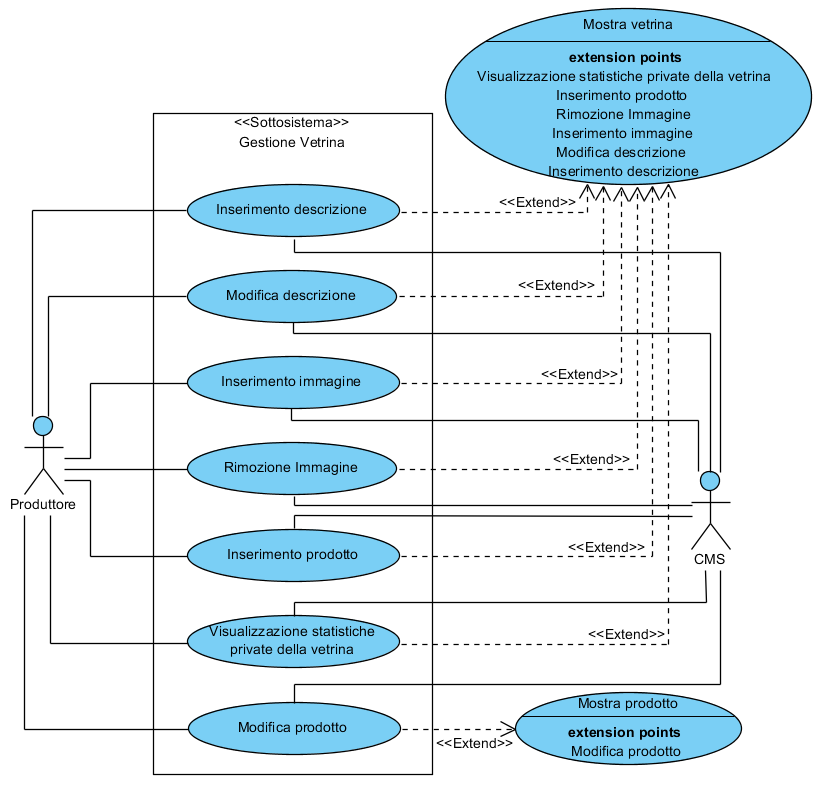
\includegraphics[width=\textwidth]{assets/visualParadigm/cu/GestioneVentrina}
\end{center}
%***************  INSERISCI DESCRIZIONE IN VETRINA *****************
\cuTab{cu:personalizzaVetrinaInsDesc}
{\getTitletodesc{att:produttore}}
{La persona connessa al sito è autenticata e ha i privilegi di Produttore. Nel sistema non è presente la descrizione della vetrina di quel Produttore. Il sistema sta mostrando alla persona la sua vetrina}
{Nel sistema è presente la descrizione della vetrina del Produttore, inserita dalla persona}
{\begin{enumCU}
		\item Il caso d'uso ha inizio quando un Produttore richiede di inserire la descrizione della sua vetrina
		\item Il sistema richiede il testo da inserire come descrizione 
		\item Il Produttore inserisce la descrizione nell'apposito campo\label{cuinsdescr:2}
		\item Il Produttore conferma il testo inserito
		\item Il sistema memorizza il testo inserito
	\end{enumCU}}
%
\cuAlternativo{cu:personalizzaVetrinaInsDesc}
{Flusso alternativo 1}%
{Annulla inserimento}%
{La persona connessa al sito è autenticata e ha i privilegi di Produttore. Nel sistema non è presente la descrizione della vetrina di quel Produttore. Il sistema sta mostrando alla persona la sua vetrina}%
{\postNulle}%
{\begin{enumCU}
		\item Dopo il punto \ref{cuinsdescr:2} il Produttore annulla l'inserimento della descrizione
	\end{enumCU}}%

\vspaceTab

\cuTab{cu:personalizzaVetrinaModDesc}
{\getTitletodesc{att:produttore}}
{La persona connessa al sito è autenticata e ha i privilegi di Produttore. Nel sistema è presente la descrizione della vetrina di quel Produttore. Il sistema sta mostrando alla persona la sua vetrina}
{Nel sistema è presente la descrizione della vetrina del Produttore, inserita dalla persona}
{\begin{enumCU}
		\item Il caso d'uso ha inizio quando un Produttore richiede di modificare la descrizione della sua vetrina
		\item Il sistema richiede il testo da inserire come descrizione, il campo in cui inserire il testo è precompilato con la descrizione già presente nel sistema 
		\item Il Produttore inserisce la descrizione nell'apposito campo\label{cumoddescr:2}
		\item Il Produttore conferma il testo inserito
		\item Il sistema memorizza il testo inserito
	\end{enumCU}}
%
\cuAlternativo{cu:personalizzaVetrinaModDesc}
{Flusso alternativo 1}%
{Annulla modifica}%
{La persona connessa al sito è autenticata e ha i privilegi di Produttore. Nel sistema è presente la descrizione della vetrina di quel Produttore. Il sistema sta mostrando alla persona la sua vetrina}%
{\postNulle}%
{\begin{enumCU}
		\item Dopo il punto \ref{cumoddescr:2} il Produttore annulla la modifica della descrizione
	\end{enumCU}}%

\vspaceTab

%***************  INSERISCI IMMAGINE IN VETRINA *****************
\cuTab{cu:personalizzaVetrinaInsImg}
{\getTitletodesc{att:produttore}}
{La persona connessa al sito è autenticata e ha i privilegi di Produttore. Il sistema sta mostrando alla persona la sua vetrina}
{Nel sistema è presente l'immagine della vetrina del Produttore, inserita dalla persona}
{\begin{enumCU}
		\item Il caso d'uso ha inizio quando un Produttore richiede di inserire l'immagine della sua vetrina
		\item Il sistema richiede il percorso nel file system, o nella rete, dell'immagine da inserire 
		\item Il Produttore inserisce il percorso dell'immagine nell'apposito campo\label{cuinsimm:2}
		\item Il Produttore conferma il percorso dell'immagine inserito\label{cuinsimm:3}
		\item Il sistema scarica e memorizza l'immagine impostandola come immagine della vetrina del Produttore
	\end{enumCU}}
%
\cuAlternativo{cu:personalizzaVetrinaInsImg}
{Flusso alternativo 1}%
{Errore inserimento}%
{La persona connessa al sito è autenticata e ha i privilegi di Produttore. Il sistema sta mostrando alla persona la sua vetrina}%
{\postNulle}%
{\begin{enumCU}
		\item Dopo il punto \ref{cuinsimm:3} il sistema non riesce a trovare, scaricare o inserire correttamente l'immagine
	\end{enumCU}}%
%
\cuAlternativo{cu:personalizzaVetrinaInsImg}
{Flusso alternativo 2}%
{Annulla inserimento}%
{La persona connessa al sito è autenticata e ha i privilegi di Produttore. Il sistema sta mostrando alla persona la sua vetrina}%
{\postNulle}%
{\begin{enumCU}
		\item Dopo il punto \ref{cuinsimm:2} il produttore annulla l'inserimento dell'immagine
	\end{enumCU}}%

\vspaceTab

\cuTab{cu:personalizzaVetrinaDelImg}
{\getTitletodesc{att:produttore}}
{La persona connessa al sito è autenticata e ha i privilegi di Produttore. Nel sistema è presente l'immagine della vetrina del Produttore. Il sistema sta mostrando alla persona la sua vetrina}
{Nel sistema non è presente l'immagine della vetrina del Produttore}
{\begin{enumCU}
		\item Il caso d'uso ha inizio quando un Produttore richiede di rimuovere l'immagine della sua vetrina
		\item Il sistema richiede di confermare l'operazione \label{cudelimm:2}
		\item Il Produttore conferma l'operazione
		\item Il sistema rimuove l'immagine della vetrina del produttore
	\end{enumCU}}

\vspaceTab

%***************  INSERISCI PRODOTTO IN VETRINA *****************
\cuTab{cu:personalizzaVetrinaInsProd}
{\getTitletodesc{att:produttore}}
{La persona connessa al sito è autenticata e ha i privilegi di Produttore. Il sistema sta mostrando alla persona la sua vetrina}
{Nella vetrina del Produttore è presente la scheda del prodotto inserito}
{\begin{enumCU}
		\item Il caso d'uso ha inizio quando un Produttore richiede di inserire un prodotto nella sua vetrina
		\item Il sistema richiede di compilare la scheda del prodotto da inserire
		\item Il Produttore inserisce i dati richiesti\label{cuinsimmpro:1}
		\item Il Produttore conferma i dati inseriti 
		\item Il sistema richiede almeno un percorso nel file system, o nella rete, dell'immagine del prodotto da inserire
		\item Il Produttore inserisce nell'apposito campo uno o più percorsi  delle immagini che vuole inserire\label{cuinsimmpro:2}
		\item Il Produttore conferma i percorsi inseriti\label{cuinsimmpro:3}
		\item Il sistema memorizza i dati e i percorsi inseriti e scarica le immagini nel sistema
	\end{enumCU}}
%
\cuAlternativo{cu:personalizzaVetrinaInsProd}
{Flusso alternativo 1}%
{Errore inserimento}%
{La persona connessa al sito è autenticata e ha i privilegi di Produttore. Il sistema sta mostrando alla persona la sua vetrina}%
{\postNulle}%
{\begin{enumCU}
		\item Dopo il punto \ref{cuinsimmpro:3} il sistema non riesce a trovare, scaricare o inserire correttamente una o più immagini
	\end{enumCU}}%
%
\cuAlternativo{cu:personalizzaVetrinaInsProd}
{Flusso alternativo 2}%
{Annulla inserimento}%
{La persona connessa al sito è autenticata e ha i privilegi di Produttore. Il sistema sta mostrando alla persona la sua vetrina}%
{\postNulle}%
{\begin{enumCU}
		\item Dopo il punto \ref{cuinsimmpro:2} o dopo il punto \ref{cuinsimmpro:1} il Produttore annulla l'inserimento della scheda prodotto
	\end{enumCU}}%

\vspaceTab

%***************  MODIFICA PRODOTTO IN VETRINA *****************
\cuTab{cu:personalizzaVetrinaModProd}
{\getTitletodesc{att:produttore}}
{La persona connessa al sito è autenticata e ha i privilegi di Produttore. Il sistema sta mostrando alla persona la scheda di un prodotto presente nella sua vetrina}%
{Nella vetrina del Produttore è stata modificara la scheda del prodotto selezionato}
{\begin{enumCU}
		\item Il caso d'uso ha inizio quando un Produttore richiede di modificare la scheda del prodotto che sta visualizzando
		\item Il sistema richiede di compilare la scheda prodotto, precompilata con i dati già presenti nel sistema
		\item Il Produttore inserisce i dati richiesti\label{cumodprodelim:1}
		\item Il Produttore conferma i dati inseriti
		\item Il sistema mostra le immagini del prodotto presenti, con la possibilità di eliminarle, e mostra i campi per aggiungere i percorsi nel file system, o nella rete, di altre immagini da aggiungere\label{cumodprodelim:3}
		\item Il Produttore inserisce i percorsi nel file system delle immagini che intende aggiungere
		\item Il Produttore conferma i percorsi inseriti\label{cumodprodelim:2}
		\item Il sistema memorizza i dati e i percorsi inseriti e scarica le immagini nel sistema
	\end{enumCU}} %%SETTARE UN PRODOTTO COME FUORI PRODUZIONE&&
%
\cuAlternativo{cu:personalizzaVetrinaModProd}
{Flusso alternativo 1}%
{Elimina immagine}%
{La persona connessa al sito è autenticata e ha i privilegi di Produttore. Il sistema sta mostrando alla persona la scheda di un prodotto con almeno due immagini presente nella sua vetrina}
{Nel sistema non è più presente l'immagine selezionata}%
{\begin{enumCU}
		\item Dopo il punto \ref{cumodprodelim:3} il Produttore seleziona un'immagine
		\item Il Produttore richiede la rimozione dell'immagine
		\item Il sistema accetta l'operazione
	\end{enumCU}}%
%
\cuAlternativo{cu:personalizzaVetrinaModProd}
{Flusso alternativo 2}%
{Annulla Modifica}%
{La persona connessa al sito è autenticata e ha i privilegi di Produttore. Il sistema sta mostrando alla persona la scheda di un prodotto presente nella sua vetrina}%
{\postNulle}%
{\begin{enumCU}
		\item Dopo il punto \ref{cumodprodelim:2} o dopo il punto \ref{cumodprodelim:1} il Produttore annulla l'inserimento della scheda del prodotto
	\end{enumCU}}%

\vspaceTab

%***************  STATISTICHE PRIVATE VETRINA *****************
\cuTab{cu:statistichePrivateVetrina}
{\getTitletodesc{att:produttore}}
{La persona connessa al sito è autenticata e ha i privilegi di Produttore. Il sistema sta mostrando alla persona la sua vetrina}
{Il sistema sta mostrando al Produttore le statistiche private della propria vetrina}
{\begin{enumCU}
		\item Il caso d'uso ha inizio quando un Produttore richiede di accedere alle statistiche private della sua vetrina
		\item Il sistema mostra al Produttore le statistiche della sua vetrina
	\end{enumCU}}

\subsection{Gestione notizie}
\begin{center}
   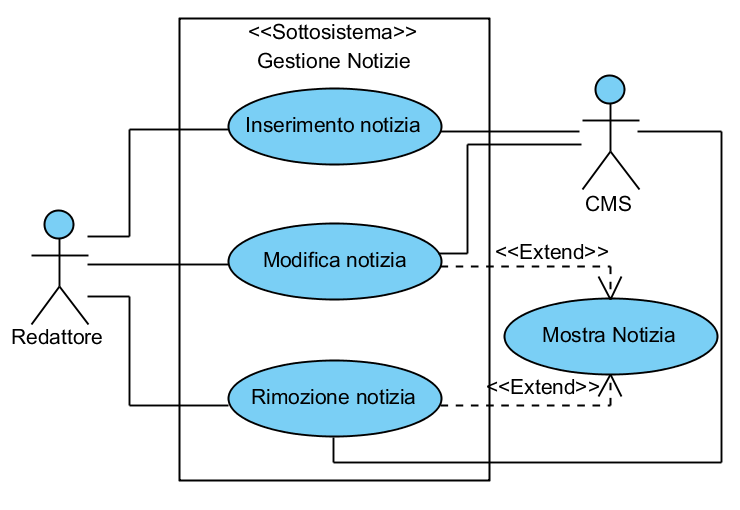
\includegraphics[width=\textwidth]{assets/visualParadigm/cu/GestioneNotizie}
\end{center}
%
%***************  INSERIMENTO NOTIZIA *****************
\cuTab{cu:inserimentoNotizia}
{\getTitletodesc{att:redattore}}
{La persona connessa al sito è autenticata e ha i privilegi di Redattore}
{Nel sistema è presente la notizia inserita}
{\begin{enumCU}
	\item Il caso d'uso ha inizio quando un Redattore richiede di inserire una notizia  
	\item Il sistema richiede di compilare i campi necessari all'inserimento della notizia
	\item Il Redattore inserisce i dati richiesti \label{cuinsnot:2}
	\item Il Redattore conferma i dati richiesti
	\item Il sistema memorizza i dati inseriti e crea una nuova notizia
\end{enumCU}}
%
\cuAlternativo{cu:inserimentoNotizia}
{Flusso alternativo 1}%
{Annulla inserimento}%
{La persona connessa al sito è autenticata e ha i privilegi di Redattore}%
{\postNulle}%
{\begin{enumCU}
		\item Dopo il punto \ref{cuinsnot:2} il Redattore annulla l'inserimento della notizia
	\end{enumCU}}%

\vspaceTab

%***************  MODIFICA NOTIZIA *****************
\cuTab{cu:modificaNotizia}
{\getTitletodesc{att:redattore}}
{La persona connessa al sito è autenticata e ha i privilegi di Redattore. Il sistema sta mostrando alla persona una notizia}
{Nel sistema la notizia viene modificata correttamente}
{\begin{enumCU}
	\item Il caso d'uso ha inizio quando un Redattore richiede di modificare la notizia che sta visualizzando
	\item Il sistema richiede di compilarne la scheda associata, precompilata con i dati già presenti nel sistema 
	\item Il Redattore inserisce, modifica o lascia inalterati i dati richiesti\label{cumodnot:2}
	\item Il Redattore conferma i dati richiesti
	\item Il sistema memorizza i dati inseriti e modifica la notizia
\end{enumCU}}
%
\cuAlternativo{cu:modificaNotizia}
{Flusso alternativo 1}%
{Annulla modifica}%
{La persona connessa al sito è autenticata e ha i privilegi di Redattore. Il sistema sta mostrando alla persona una notizia}%
{\postNulle}%
{\begin{enumCU}
		\item Dopo il punto \ref{cumodnot:2} il Redattore annulla la modifica della notizia
\end{enumCU}}%

\vspaceTab

%***************  RIMOZIONE NOTIZIA *****************
\cuTab{cu:rimozioneNotizia}
{\getTitletodesc{att:redattore}}
{La persona connessa al sito è autenticata e ha i privilegi di Redattore. Il sistema sta mostrando alla persona una notizia}
{Nel sistema non è più presente la notizia}
{\begin{enumCU}
	\item Il caso d'uso ha inizio quando un Redattore richiede di rimuovere la notizia che sta visualizzando
	\item Il sistema chiede conferma della rimozione\label{curemnot:2}
	\item Il Redattore conferma la rimozione
	\item Il sistema rimuove la notizia selezionata
\end{enumCU}}
%
\cuAlternativo{cu:rimozioneNotizia}
{Flusso alternativo 1}%
{Annulla rimozione}%
{La persona connessa al sito è autenticata e ha i privilegi di Redattore. Il sistema sta mostrando alla persona una notizia}%
{\postNulle}%
{\begin{enumCU}
		\item Dopo il punto \ref{curemnot:2} il Redattore annulla la rimozione della notizia
	\end{enumCU}}%

\subsection{Gestione suggerimenti}
\begin{center}
   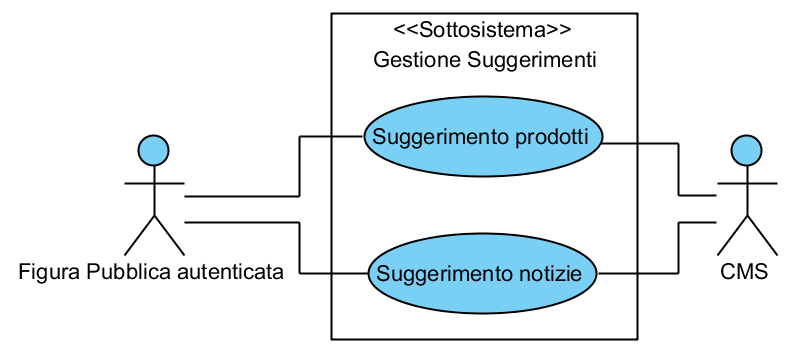
\includegraphics[width=\textwidth]{assets/visualParadigm/cu/GestioneSuggerimenti}
\end{center}
%***************  SUGGERIMENTO PRODOTTI *****************
%Accorpa suggerimento intelligente e simili
\cuTab{cu:suggerimentoProdotti}
{\getTitletodesc{att:figuraPubblicaAutenticata}}
{La persona connessa al sito è autenticata ed ha i privilegi di Figura Pubblica Autenticata. Il sistema sta mostrando alla persona la scheda di un prodotto}
{Il sistema sta mostrando alla persona una lista di \glspl{anteprima} di prodotti simili}
{\begin{enumCU}
	\item Il caso d'uso ha inizio quando una Figura Pubblica Autenticata richiede di mostrare le \glspl{anteprima} delle schede di prodotti simili a quella che sta visualizzando
	\item Il sistema mostra alla Figura Pubblica Autenticata una lista di \glspl{anteprima} di prodotti simili
\end{enumCU}}

\vspaceTab

%***************  SUGGERIMENTO NOTIZIE *****************
\cuTab{cu:notizieSimili}
{\getTitletodesc{att:figuraPubblicaAutenticata}}
{La persona connessa al sito è autenticata ed ha i privilegi di Figura Pubblica Autenticata. Il sistema sta mostrando alla persona la scheda di un prodotto}
{Il sistema sta mostrando alla persona una lista di \glspl{anteprima} di notizie simili}
{\begin{enumCU}
	\item Il caso d'uso ha inizio quando una Figura Pubblica Autenticata richiede di mostrare notizie simili alla notizia che sta visualizzando
	\item Il sistema mostra alla Figura Pubblica Autenticata una lista di \glspl{anteprima} di notizie simili
\end{enumCU}}

\subsection{Gestione account}
\begin{center}
   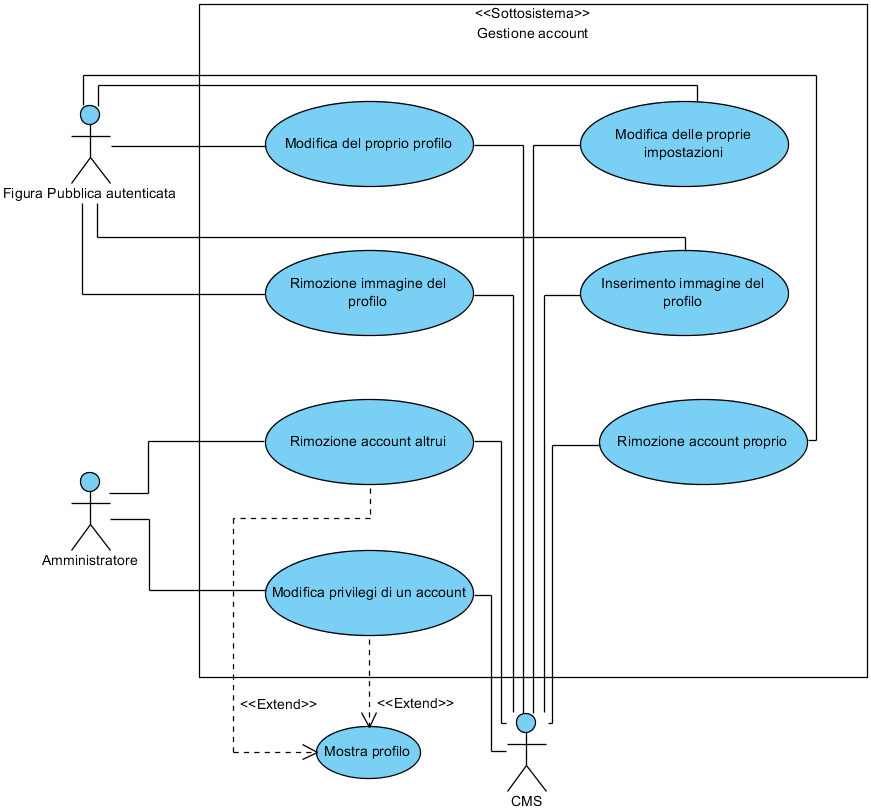
\includegraphics[width=\textwidth]{assets/visualParadigm/cu/GestioneAccount}
\end{center}
%***************  ACCESSO PROFILO *****************
\cuTab{cu:modificaProfilo}
{\getTitletodesc{att:figuraPubblicaAutenticata}, \getTitletodesc{att:figuraAmministrativa}}
{La persona connessa al sito è autenticata. Il sistema sta mostrando alla persona il suo profilo}
{Il profilo della persona è stato modificato}
{\begin{enumCU}
	\item Il caso d'uso ha inizio quando una persona autenticata nel sistema richiede di modificare il proprio profilo
	\item Il sistema mostra alla persona i campi modificabili
	\item La persona effettua le modifiche volute \label{modProf}
	\item La persona conferma le modifiche effettuate
	\item Il sistema memorizza le modifiche
\end{enumCU}}
%
\cuAlternativo{cu:modificaProfilo}
{Flusso alternativo 1}%
{Annulla modifica}%
{La persona connessa al sito è autenticata. Il sistema sta mostrando alla persona il suo profilo}
{\postNulle}%
{\begin{enumCU}
	\item Dopo il punto \ref{modProf} annulla le modifiche effettuate
\end{enumCU}}%

\vspaceTab

\cuTab{cu:inserisciImgProfilo}
{\getTitletodesc{att:figuraPubblicaAutenticata}, \getTitletodesc{att:figuraAmministrativa}}
{La persona connessa al sito è autenticata. Il sistema sta mostrando alla persona il suo profilo}
{Nel sistema è presente l'immagine del profilo della persona}
{\begin{enumCU}
	\item Il caso d'uso ha inizio quando una persona autenticata nel sistema richiede di inserire l'immagine del proprio profilo
	\item Il sistema richiede il percorso nel file system, o nella rete, dell'immagine da inserire 
	\item La persona inserisce il percorso dell'immagine nell'apposito campo\label{insimg1}
	\item La persona conferma il percorso dell'immagine inserito\label{insimg2}
	\item Il sistema scarica e memorizza l'immagine impostandola come immagine del profilo della persona
\end{enumCU}}
%
\cuAlternativo{cu:inserisciImgProfilo}
{Flusso alternativo 1}%
{Errore inserimento}%
{La persona connessa al sito è autenticata. Il sistema sta mostrando alla persona il suo profilo}
{\postNulle}%
{\begin{enumCU}
		\item Dopo il punto \ref{insimg2} il sistema non riesce a trovare, scaricare o inserire correttamente l'immagine
	\end{enumCU}}%
%
\cuAlternativo{cu:inserisciImgProfilo}
{Flusso alternativo 2}%
{Annulla inserimento}%
{La persona connessa al sito è autenticata. Il sistema sta mostrando alla persona il suo profilo}
{\postNulle}%
{\begin{enumCU}
		\item Dopo il punto \ref{insimg1} il produttore annulla l'inserimento dell'immagine
	\end{enumCU}}%

\vspaceTab

\cuTab{cu:rimuoviImgProfilo}
{\getTitletodesc{att:figuraPubblicaAutenticata}, \getTitletodesc{att:figuraAmministrativa}}
{La persona connessa al sito è autenticata. Il sistema sta mostrando alla persona il suo profilo. Nel sistema è presente l'immagine del profilo della persona}
{Nel sistema non è presente l'immagine del profilo della persona}
{\begin{enumCU}
	\item Il caso d'uso ha inizio quando una persona autenticata nel sistema richiede di rimuovere l'immagine del proprio profilo
	\item Il sistema richiede conferma della rimozione\label{annrimimg}
	\item La persona conferma la rimozione
	\item Il sistema rimuove l'immagine
\end{enumCU}}
%
\cuAlternativo{cu:rimuoviImgProfilo}
{Flusso alternativo 1}%
{Annulla rimozione}%
{La persona connessa al sito è autenticata. Il sistema sta mostrando alla persona il suo profilo. Nel sistema è presente l'immagine del profilo della persona}
{\postNulle}%
{\begin{enumCU}
		\item Dopo il punto \ref{annrimimg} la persona annulla l'operazione di rimozione
	\end{enumCU}}%

\vspaceTab

%***************  ACCESSO IMPOSTAZIONI *****************
\cuTab{cu:modificaImpostazioni}
{\getTitletodesc{att:figuraPubblicaAutenticata}, \getTitletodesc{att:figuraAmministrativa}}
{La persona connessa al sito è autenticata}
{Nel sistema le impostazioni della persona sono state modificate come richiesto}   
{\begin{enumCU}
	\item Il caso d'uso ha inizio quando una persona autenticata nel sistema richiede di modificare la pagina delle proprie impostazioni
	\item Il sistema mostra alla persona la pagina delle proprie impostazioni, abilitando solo i campi che la persona può modificare
	\item La persona modifica i campi presenti nella pagina\label{cumodimp:1}
	\item La persona conferma le modifiche effettuate 
	\item Il sistema memorizza le modifiche effettuate
\end{enumCU}
\ext{cu:rimozioneAccountProprio}}
%
\cuAlternativo{cu:modificaImpostazioni}
{Flusso alternativo 1}%
{Annulla modifica}%
{La persona connessa al sito è autenticata nel sistema}%
{\postNulle}%
{\begin{enumCU}
		\item Dopo il punto \ref{cumodimp:1} annulla le modifiche effettuate
	\end{enumCU}}%

\vspaceTab

%***************  RIMOZIONE ACCOUNT PROPRIO  *****************
\cuTab{cu:rimozioneAccountProprio}
{\getTitletodesc{att:figuraPubblicaAutenticata}}
{La persona connessa al sito è autenticata ed ha solo i privilegi di Figura Pubblica Autenticata}
{La persona non è più autenticata nel sistema. L'account della persona non è più presente nel sistema}
{\begin{enumCU}
	\item Il caso d'uso ha inizio quando una Figura Pubblica Autenticata nel sistema richiede di rimuovere il proprio account
	\item Il sistema chiede conferma della rimozione dell'account\label{curimaccprop:1}
	\item La persona conferma la rimozione
	\item Il sistema rimuove l'account del richiedente
\end{enumCU}}
%
\cuAlternativo{cu:rimozioneAccountProprio}
{Flusso alternativo 1}%
{Annulla rimozione}%
{La persona connessa al sito è autenticata ed ha solo i privilegi di Figura Pubblica Autenticata}%
{\postNulle}%
{\begin{enumCU}
		\item Dopo il punto \ref{curimaccprop:1} la persona annulla la rimozione dell'account
	\end{enumCU}}%

\vspaceTab

%***************  RIMOZIONE ACCOUNT ALTRUI  *****************
\cuTab{cu:rimozioneAccountAltrui}
{\getTitletodesc{att:amministratore}}
{La persona connessa al sito è autenticata e ha i privilegi di Amministratore. Il sistema sta mostrando alla persona un profilo associato ad un altro account}
{Nel sistema non è più presente l'account rimosso}
{\begin{enumCU}
	\item Il caso d'uso ha inizio quando un Amministratore richiede al sistema di rimuovere l'account associato al profilo che sta visualizzando
	\item Il sistema chiede conferma della rimozione dell'account\label{curimaccaltr:1}
	\item L'Amministratore conferma la rimozione
	\item Il sistema rimuove l'account selezionato
\end{enumCU}}
%
\cuAlternativo{cu:rimozioneAccountAltrui}
{Flusso alternativo 1}%
{Annulla rimozione}%
{La persona connessa al sito è autenticata e ha i privilegi di Amministratore. Il sistema sta mostrando alla persona un profilo associato ad un altro account}%
{\postNulle}%
{\begin{enumCU}
	\item Dopo il punto \ref{curimaccaltr:1} l'Amministratore annulla la rimozione dell'account
\end{enumCU}}%

\vspaceTab

%***************  Modifica privilegi  *****************
\cuTab{cu:modificaPrivilegiAccount}
{\getTitletodesc{att:amministratore}}
{La persona connessa al sito è autenticata e ha i privilegi di Amministratore. Il sistema sta mostrando alla persona una lista di \glspl{anteprima} di profili}
{Nel sistema sono stati aggiornati i privilegi di quell'account come richiesto}
{\begin{enumCU}
	\item Il caso d'uso ha inizio quando un Amministratore seleziona un'\gls{anteprima} profilo tra quelle mostrate nel risultato della ricerca e richiede di modificarne i privilegi
	\item Il sistema mostra all'Amministratore la lista dei privilegi, specificando quelli posseduti dall'account associato al profilo selezionato
	\item Il sistema chiede di modificare i privilegi posseduti dall'account
	\item L'Amministratore seleziona quali privilegi vuole fornire all'account\label{cufornpriv:1}
	\item L'Amministratore conferma la selezione
	\item Il sistema memorizza le scelte effettuate
\end{enumCU}}
%
\cuAlternativo{cu:modificaPrivilegiAccount}
{Flusso alternativo 1}%
{Annulla operazione}%
{La persona connessa al sito è autenticata e ha i privilegi di Amministratore. Il sistema sta mostrando alla persona una lista di \glspl{anteprima} di profili}%
{\postNulle}%
{\begin{enumCU}
		\item Dopo il punto \ref{cufornpriv:1} l'Amministratore annulla l'operazione
	\end{enumCU}}%

\vspaceTab

%***************  Gestione valutazioni *****************
\subsection{Gestione valutazioni}
\begin{center}
   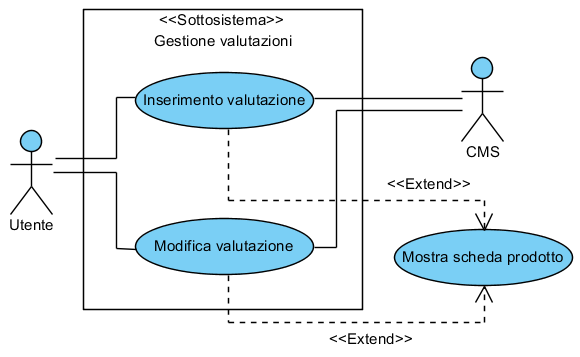
\includegraphics[width=\textwidth]{assets/visualParadigm/cu/GestioneValutazioni}
\end{center}
\cuTab{cu:inserisciValutazioneProdotto}
{\getTitletodesc{att:utente}}
{La persona connessa al sito è autenticata ed ha i privilegi di Utente. Il sistema sta mostrando alla persona la scheda di un prodotto che non ha già stato valutato}
{Nel sistema è stata aggiunta la valutazione della persona per il prodotto}
{\begin{enumCU}
	\item Il caso d'uso ha inizio quando un Utente richiede di effettuare la valutazione del prodotto che sta visualizzando
	\item Il sistema richiede all'Utente la valutazione per quel prodotto
	\item L'Utente inserisce la valutazione
	\item Il sistema memorizza la valutazione
\end{enumCU}
\ext{cu:inserisciRecensioneProdotto}
}


\vspaceTab

\cuTab{cu:modificaValutazioneProdotto}
{\getTitletodesc{att:utente}}
{La persona connessa al sito è autenticata ed ha i privilegi di Utente. Il sistema sta mostrando alla persona la scheda di un prodotto che ha già stato valutato}
{Nel sistema è stata modificata la valutazione del prodotto inserita dalla persona}
{\begin{enumCU}
	\item Il caso d'uso ha inizio quando un Utente richiede di modificare la valutazione del prodotto
	\item Il sistema mostra all'Utente la valutazione che ha effettuato per quel prodotto
	\item L'Utente inserisce la nuova valutazione
	\item Il sistema memorizza la nuova valutazione inserita
\end{enumCU}}

%***************  Gestione recensione *****************
\subsection{Gestione recensioni}
\begin{center}
   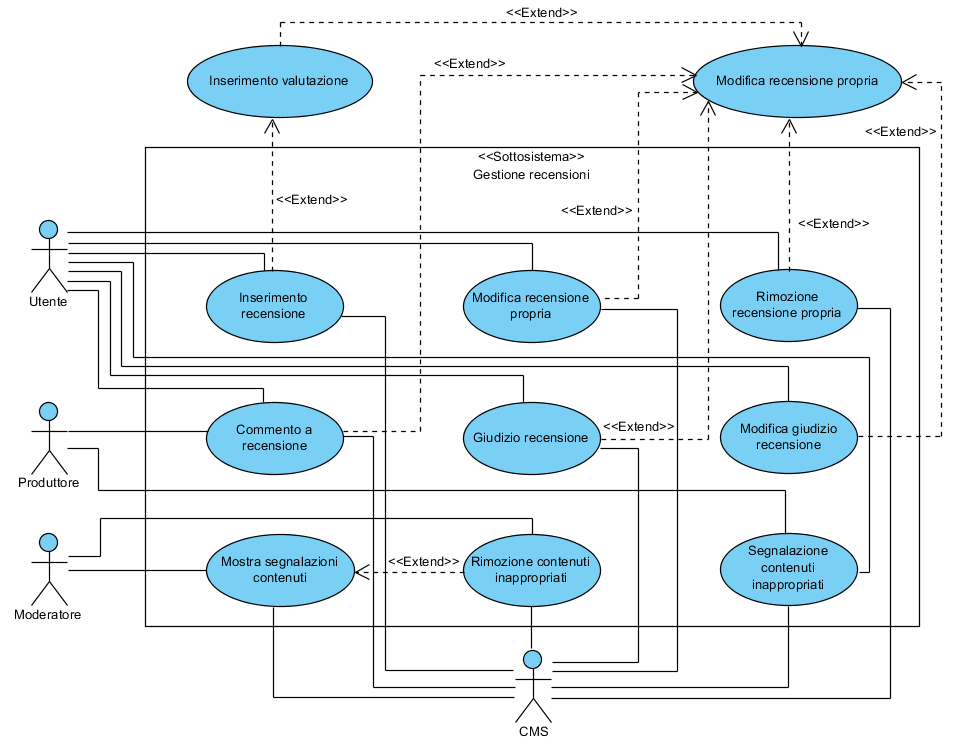
\includegraphics[width=\textwidth]{assets/visualParadigm/cu/GestioneRecensioni}
\end{center}
\cuTab{cu:inserisciRecensioneProdotto}
{\getTitletodesc{att:utente}}
{La persona connessa al sito è autenticata come Utente. Il sistema sta mostrando alla persona la scheda di un prodotto che ha già stato valutato}
{Nel sistema è presente la recensione dell'Utente per quel prodotto}
{\begin{enumCU}
	\item Il caso d'uso ha inizio quando un Utente richiede di effettuare la recensione del prodotto che sta visualizzando
	\item Il sistema richiede all'Utente il testo da inserire come recensione
	\item L'Utente inserisce la recensione\label{addrec:3}
	\item L'Utente conferma la recensione inserita
	\item Il sistema memorizza la recensione
\end{enumCU}}
%
\cuAlternativo{cu:inserisciRecensioneProdotto}
{Flusso alternativo 1}%
{Annulla inserimento}%
{La persona connessa al sito è autenticata come Utente. Il sistema sta mostrando alla persona la scheda di un prodotto che ha già stato valutato}%
{\postNulle}%
{\begin{enumCU}
		\item Dopo il punto \ref{addrec:3}, l'Utente annulla l'operazione di inserimento
	\end{enumCU}}%

\vspaceTab

\cuTab{cu:modificaRecensioneProdotto}
{\getTitletodesc{att:utente}}
{La persona connessa al sito è autenticata come Utente. Il sistema sta mostrando alla persona una recensione di un prodotto che ha effettuato}
{Nel sistema è stata modificata la recensione di quella persona per quel prodotto}
{\begin{enumCU}
	\item Il caso d'uso ha inizio quando un Utente richiede di modificare la recensione che sta visualizzando
	\item Il sistema mostra all'Utente la recensione che ha effettuato per quel prodotto
	\item L'Utente inserisce la nuova recensione \label{newrec:3}
	\item L'Utente conferma la nuova recensione inserita
	\item Il sistema memorizza la nuova recensione
\end{enumCU}}
%
\cuAlternativo{cu:modificaRecensioneProdotto}
{Flusso alternativo 1}%
{Annulla modifiche}%
{La persona connessa al sito è autenticata come Utente. Il sistema sta mostrando alla persona una recensione di un prodotto che ha effettuato}
{\postNulle}%
{\begin{enumCU}
		\item Dopo il punto \ref{newrec:3}, l'Utente annulla l'operazione di modifica
	\end{enumCU}}%

\vspaceTab

\cuTab{cu:eliminaRecensioneProdotto}
{\getTitletodesc{att:utente}}
{La persona connessa al sito è autenticata  come Utente. Il sistema sta mostrando alla persona una recensione di un prodotto che ha effettuato}
{Nel sistema è stata rimossa la recensione di quella persona}
{\begin{enumCU}
	\item Il caso d'uso ha inizio quando un Utente richiede di rimuovere la recensione per quel prodotto
	\item Il sistema mostra all'Utente la recensione che ha effettuato per quel prodotto
	\item Il sistema richiede di confermare la rimozione \label{remrec:3}
	\item L'Utente conferma la rimozione
	\item Il sistema rimuove la recensione
\end{enumCU}}
%
\cuAlternativo{cu:eliminaRecensioneProdotto}
{Flusso alternativo 1}%
{Annulla rimozione}%
{La persona connessa al sito è autenticata  come Utente. Il sistema sta mostrando alla persona una recensione di un prodotto effettuata dalla persona}
{\postNulle}%
{\begin{enumCU}
		\item Dopo il punto \ref{remrec:3}, l'Utente annulla l'operazione di rimozione
	\end{enumCU}}%

\vspaceTab

\cuTab{cu:commentoRecensione}
{\getTitletodesc{att:figuraPubblicaAutenticata}}
{La persona è connessa al sito ed ha i privilegi di Figura Pubblica Autenticata. Il sistema sta mostrando alla persona la recensione di un prodotto}
{Nel sistema è presente il commento inserito dalla persona per quella recensione}
{\begin{enumCU}
	\item Il caso d'uso ha inizio quando la persona richiede di effettuare un commento alla recensione che sta visualizzando\label{commrifiutato2}
	\item Il sistema mostra alla persona la recensione e i commenti relativi ad essa
	\item Il sistema richiede di inserire un nuovo commento 
	\item La persona inserisce il commento\label{addcom:3}
	\item La persona conferma il commento inserito
	\item Il sistema memorizza il commento
\end{enumCU}}
%
\cuAlternativo{cu:commentoRecensione}
{Flusso alternativo 1}%
{Annulla rimozione}%
{La persona è connessa al sito ed ha i privilegi di Figura Pubblica Autenticata. Il sistema sta mostrando alla persona la recensione di un prodotto}
{\postNulle}%
{\begin{enumCU}
		\item Dopo il punto \ref{addcom:3}, la persona annulla l'operazione di inserimento
	\end{enumCU}}%
%
\cuAlternativo{cu:commentoRecensione}
{Flusso alternativo 2}%
{Errore inserimento}%
{La persona è connessa al sito ed ha i privilegi di Produttore. Il sistema sta mostrando alla persona la recensione di un prodotto}
{\postNulle}%
{\begin{enumCU}
		\item Nel punto \ref{commrifiutato2} la persona richiede di effettuare un commento alla recensione che sta visualizzando, di un prodotto non suo
		\item Dopo il punto \ref{commrifiutato2} il sistema rifiuta la richiesta
	\end{enumCU}}%

\vspaceTab

\cuTab{cu:giudizioRecensione}
{\getTitletodesc{att:utente}}
{La persona connessa al sito è autenticata come Utente. Il sistema sta mostrando alla persona la recensione di un prodotto che non ha giudicato}
{Nel sistema è presente il giudizio di quella persona per quella recensione}
{\begin{enumCU}
	\item Il caso d'uso ha inizio quando un Utente richiede di esprimere un giudizio (positivo o negativo) sulla recensione che sta visualizzando
	\item Il sistema mostra all'Utente la recensione
	\item Il sistema richiede all'Utente il giudizio per quella recensione
	\item L'Utente inserisce il giudizio
	\item Il sistema memorizza il giudizio
\end{enumCU}}


\cuTab{cu:modificaGiudizioRecensione}
{\getTitletodesc{att:utente}}
{La persona connessa al sito è autenticata  come Utente. Il sistema sta mostrando alla persona la recensione di un prodotto che ha già giudicato}
{Nel sistema è stato modificato il giudizio di quella persona per quella recensione}
{\begin{enumCU}
	\item Il caso d'uso ha inizio quando un Utente richiede di modificare un giudizio della recensione che sta visualizzando
	\item Il sistema mostra all'Utente la recensione
	\item Il sistema mostra all'Utente il suo giudizio per quella recensione
	\item Il sistema richiede all'Utente il nuovo giudizio per quella recensione
	\item L'Utente inserisce il nuovo giudizio
	\item Il sistema memorizza il nuovo giudizio
\end{enumCU}}

\vspaceTab

\cuTab{cu:segnalazioneContenutiInap}
{\getTitletodesc{att:figuraPubblicaAutenticata}}
{La persona è connessa al sito ed ha i privilegi di Figura Pubblica Autenticata. Il sistema sta mostrando alla persona un \gls{contenuto}}
{Nel sistema è presente la segnalazione di quella persona per quel \gls{contenuto}}
{\begin{enumCU}
	\item Il caso d'uso ha inizio quando una persona richiede di segnalare il \gls{contenuto} che sta visualizzando in quanto inappropriato
	\item Il sistema richiede alla persona di specificare il motivo della segnalazione
	\item La persona inserisce il motivo della segnalazione\label{annullasegn}
	\item La persona conferma la segnalazione
	\item Il sistema memorizza la segnalazione allegando un \gls{riferimento} al \gls{contenuto} segnalato
\end{enumCU}}
%
\cuAlternativo{cu:segnalazioneContenutiInap}
{Flusso alternativo 1}%
{Annulla segnalazione}%
{La persona è connessa al sito ed ha i privilegi di Figura Pubblica Autenticata. Il sistema sta mostrando alla persona un \gls{contenuto}}
{\postNulle}%
{\begin{enumCU}
		\item Dopo il punto \ref{annullasegn}, la persona annulla l'operazione di segnalazione
	\end{enumCU}}%

\vspaceTab

\cuTab{cu:mostraSegnContenutiInap}
{\getTitletodesc{att:moderatore}}
{La persona connessa al sito è autenticata  ed ha i privilegi di Moderatore. Nel sistema è presente almeno una segnalazione}
{Il sistema sta mostrando alla persona il \gls{contenuto} segnalato}
{\begin{enumCU}
	\item Il caso d'uso ha inizio quando un Moderatore richiede di visualizzare una segnalazione
	\item Il sistema mostra al Moderatore le segnalazioni presenti nel sistema\label{delsegn:3}
	\item Il Moderatore seleziona una segnalazione tra quelle proposte
	\item Il sistema mostra la segnalazione \label{delsegn:4}
	\item Il Moderatore richiede di visualizzare il \gls{contenuto} segnalato
	\item Il sistema mostra il \gls{contenuto} segnalato
\end{enumCU}
\ext{cu:rimozioneContenutiInap}
}
%
\cuAlternativo{cu:mostraSegnContenutiInap}
{Flusso alternativo 1}%
{Elimina segnalazione}%
{La persona connessa al sito è autenticata  ed ha i privilegi di Moderatore. Nel sistema è presente almeno una segnalazione}
{Nel sistema non è più presente quella segnalazione}%
{\begin{enumCU}
		\item Dopo il punto \ref{delsegn:4}, il Moderatore elimina la segnalazione
\end{enumCU}}%
%marcare segnalazione come risolta/eliminarla dalla lista
%	
\cuAlternativo{cu:mostraSegnContenutiInap}
{Flusso alternativo 2}%
{Annulla operazione di selezione}%
{La persona connessa al sito è autenticata ed ha i privilegi di Moderatore. Nel sistema è presente almeno una segnalazione}%
{\postNulle}%
{\begin{enumCU}
		\item Dopo il punto \ref{delsegn:3} la persona annulla l'operazione di selezione
\end{enumCU}}%

\vspaceTab

\cuTab{cu:rimozioneContenutiInap}
{\getTitletodesc{att:moderatore}}
{La persona connessa al sito è autenticata ed ha i privilegi di Moderatore. Il sistema sta mostrando alla persona un \gls{contenuto}}
{Nel sistema non è più presente il \gls{contenuto}}
{\begin{enumCU}
	\item Il caso d'uso ha inizio quando un Moderatore richiede di rimuovere il \gls{contenuto} che sta visualizzando\label{rim2}
	\item Il sistema richiede al Moderatore di confermare la rimozione\label{delcont:3}
	\item Il Moderatore conferma la rimozione 
	\item Il sistema rimuove il \gls{contenuto} inappropriato
\end{enumCU}}
%
\cuAlternativo{cu:rimozioneContenutiInap}
{Flusso alternativo 1}%
{Annulla rimozione}%
{La persona connessa al sito è autenticata ed ha i privilegi di Moderatore. Il sistema sta mostrando alla persona un \gls{contenuto}}
{\postNulle}%
{\begin{enumCU}
		\item Dopo il punto \ref{delcont:3}, il Moderatore annulla l'operazione di rimozione
\end{enumCU}}%


\subsection{Interazione tra figure}
\begin{center}
   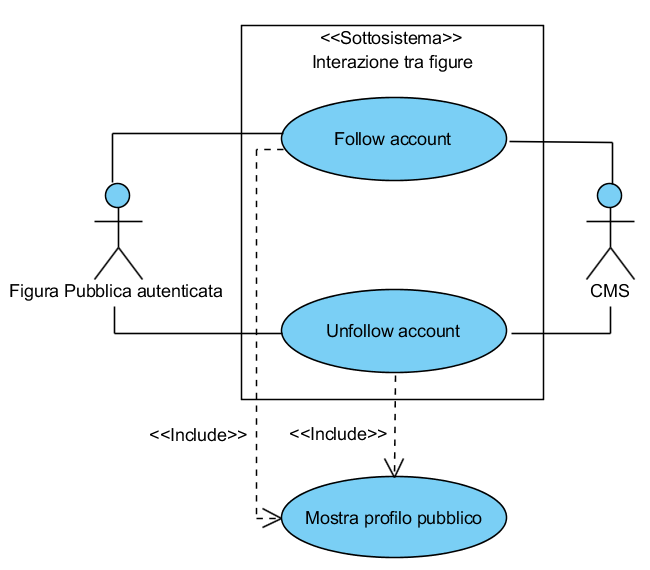
\includegraphics[width=\textwidth]{assets/visualParadigm/cu/InterazioneTraFigure}
\end{center}
%****************** FOLLOW ACCOUNT ***********
\cuTab{cu:followAccount}
{\getTitletodesc{att:figuraPubblicaAutenticata}}
{La persona è connessa al sito ed ha i privilegi di Figura Pubblica Autenticata. Il sistema sta mostrando alla persona un profilo associato ad un altro account}
{La persona segue quell'account}
{\begin{enumCU}
	\item Il caso d'uso ha inizio quando la persona richiede di seguire l'account associato al profilo visualizzato
	\item Il sistema accetta l`operazione
\end{enumCU}}

\vspaceTab

%****************** UNFOLLOW ACCOUNT ***********
\cuTab{cu:unFollowAccount}
{\getTitletodesc{att:figuraPubblicaAutenticata}}
{La persona è connessa al sito ed ha i privilegi di Figura Pubblica Autenticata. Il sistema sta mostrando alla persona un profilo associato ad un account che segue}
{La persona non segue più quell'account}
{\begin{enumCU}
	\item Il caso d'uso ha inizio quando la persona richiede di non seguire più l'account associato a quel profilo
	\item Il sistema accetta l`operazione
\end{enumCU}}

\subsection{Gestione ticket}
\begin{center}
   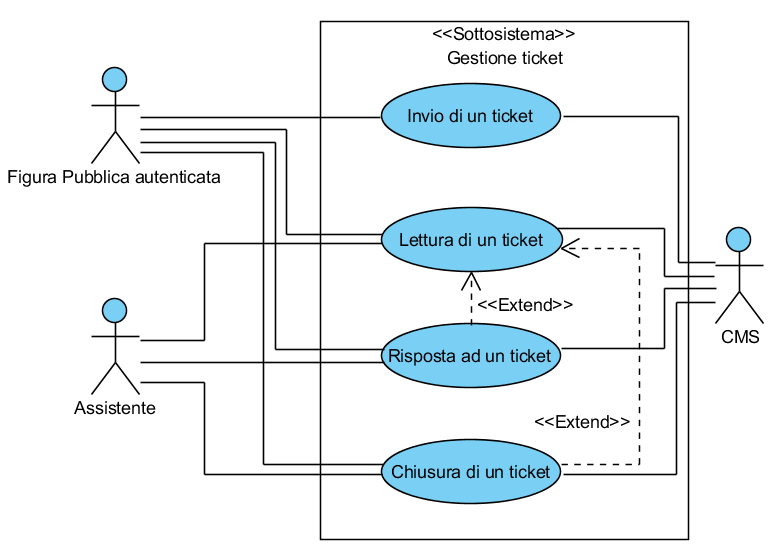
\includegraphics[width=\textwidth]{assets/visualParadigm/cu/GestioneTicket}
\end{center}
%****************** INVIO TICKET ***********
\cuTab{cu:ticketInvio}
{\getTitletodesc{att:figuraPubblicaAutenticata}}
{La persona è connessa al sito ed ha i privilegi di Figura Pubblica Autenticata}
{Nel sistema è presente il ticket creato da quella persona}
{\begin{enumCU}
	\item Il caso d'uso ha inizio quando la persona richiede la creazione di un ticket per ricevere assistenza
	\item Il sistema richiede di compilare la scheda necessaria alla creazione del ticket
	\item La persona compila la scheda\label{cucretick:1}
	\item La persona conferma i dati inseriti
	\item Il sistema memorizza il ticket
\end{enumCU}}
%
\cuAlternativo{cu:ticketInvio}
{Flusso alternativo 1}%
{Annulla creazione ticket}%
{La persona è connessa al sito ed ha i privilegi di Figura Pubblica Autenticata}%
{\postNulle}%
{\begin{enumCU}
		\item Dopo il punto \ref{cucretick:1} la persona annulla la creazione del ticket
	\end{enumCU}}%

\vspaceTab

%****************** RISPOSTA TICKET ***********
\cuTab{cu:ticketRisposta}
{\getTitletodesc{att:figuraPubblicaAutenticata}, \getTitletodesc{att:assistente}}
{La persona è connessa al sito ed ha i privilegi di Assistente, oppure ha i privilegi di Figura Pubblica Autenticata. Il sistema sta mostrando alla persona un ticket. Se la persona è una Figura Pubblica Autenticata deve essere il creatore del ticket mostrato}
{Nel sistema è presente la risposta al ticket in questione}
{\begin{enumCU}
	\item Il caso d'uso ha inizio quando la persona richiede di rispondere a quel ticket
	\item Il sistema richiede di compilare la scheda necessaria alla creazione della risposta
	\item La persona compila la scheda necessaria all'inserimento della risposta\label{curisptick:1}
	\item La persona conferma i dati inseriti
	\item Il sistema memorizza la risposta al ticket
\end{enumCU}}
%
\cuAlternativo{cu:ticketRisposta}
{Flusso alternativo 1}%
{Annulla risposta ticket}%
{La persona è connessa al sito ed ha i privilegi di Assistente, oppure ha i privilegi di Figura Pubblica Autenticata. Il sistema sta mostrando alla persona un ticket. Se la persona è una Figura Pubblica Autenticata deve essere il creatore del ticket mostrato}%
{\postNulle}%
{\begin{enumCU}
		\item Dopo il punto \ref{curisptick:1} la persona annulla l'inserimento della risposta
	\end{enumCU}}%

\vspaceTab

%****************** CHIUDI TICKET ***********
\cuTab{cu:ticketChiudi}
{\getTitletodesc{att:figuraPubblicaAutenticata}, \getTitletodesc{att:assistente}}
{La persona è connessa al sito ed ha i privilegi di Assistente, oppure ha i privilegi di Figura Pubblica Autenticata. Il sistema sta mostrando alla persona un ticket. Se la persona è una Figura Pubblica Autenticata deve essere il creatore del ticket mostrato}
{Il ticket in questione risulta chiuso nel sistema}
{\begin{enumCU}
	\item Il caso d'uso ha inizio quando la persona richiede di chiudere il ticket\label{cuchiutick:0}
	\item Il sistema richiede conferma della chiusura\label{cuchiutick:1}
	\item La persona conferma la chiusura del ticket
	\item Il sistema accetta l'operazione e memorizza il ticket come chiuso
\end{enumCU}}
%
\cuAlternativo{cu:ticketChiudi}
{Flusso alternativo 1}%
{Annulla chiusura ticket}%
{La persona è connessa al sito ed ha i privilegi di Assistente, oppure ha i privilegi di Figura Pubblica Autenticata. Il sistema sta mostrando alla persona un ticket. Se la persona è una Figura Pubblica Autenticata deve essere il creatore del ticket mostrato}%
{\postNulle}%
{\begin{enumCU}
		\item Dopo il punto \ref{cuchiutick:1} la persona annulla l'operazione di chiusura
	\end{enumCU}}%

\vspaceTab

%****************** LEGGI TICKET ***********
\cuTab{cu:ticketLettura}
{\getTitletodesc{att:figuraPubblicaAutenticata}, \getTitletodesc{att:assistente}}
{La persona è connessa al sito ed ha i privilegi di Assistente, oppure ha i privilegi di Figura Pubblica Autenticata ed è il creatore di un ticket}
{Il sistema sta mostrando alla persona il ticket}
{\begin{enumCU}
	\item Il caso d'uso ha inizio quando la persona richiede di visualizzare un ticket
	\item Il sistema mostra alla persona i ticket a cui ha accesso\label{annsel}
	\item La persona seleziona un ticket
	\item Il sistema mostra il ticket alla persona
\end{enumCU}
\ext{cu:ticketRisposta}
\ext{cu:ticketChiudi}
}
%	
\cuAlternativo{cu:ticketLettura}
{Flusso alternativo 1}%
{Annulla operazione di selezione}%
{La persona è connessa al sito ed ha i privilegi di Assistente, oppure ha i privilegi di Figura Pubblica Autenticata ed è il creatore di un ticket}%
{\postNulle}%
{\begin{enumCU}
		\item Dopo il punto \ref{annsel} la persona annulla l'operazione di selezione
\end{enumCU}}%


\subsection{Ricerca contenuti}
\begin{center}
   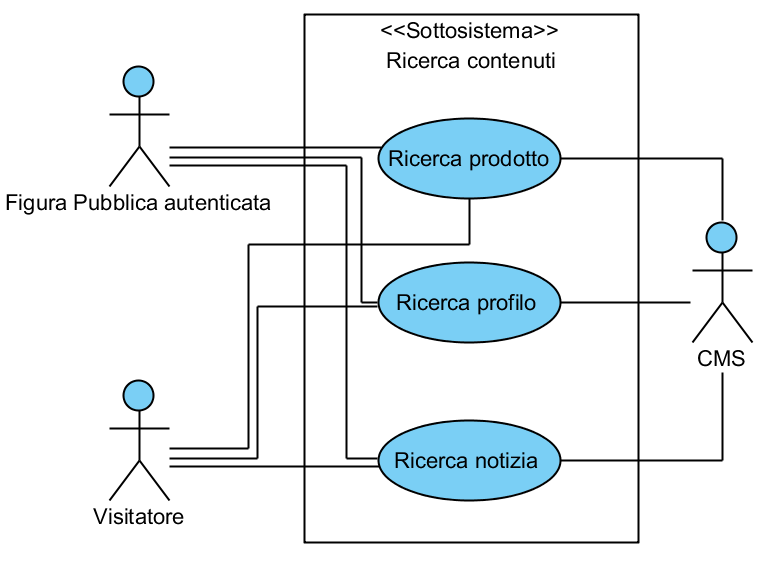
\includegraphics[width=\textwidth]{assets/visualParadigm/cu/RicercaContenuti}
\end{center}
%****************** RICERCA PRODOTTO ***********
\cuTab{cu:ricercaProdotto}
{\getTitletodesc{att:visitatore}, \getTitletodesc{att:figuraPubblicaAutenticata}}
{La persona è connessa al sito}
{Il sistema sta mostrando alla persona la lista delle \glspl{anteprima} delle schede dei prodotti cercati}
{\begin{enumCU}
	\item Il caso d'uso ha inizio quando la persona richiede di effettuare la ricerca della scheda di un prodotto
	\item Il sistema richiede di complilare la scheda necessaria per definire i parametri di ricerca
	\item La persona inserisce i dati negli appositi campi \label{curicprod:1}
	\item La persona conferma i dati inseriti
	\item Il sistema effettua la ricerca richiesta
	\item Il sistema mostra le \glspl{anteprima} dei risultati della ricerca
\end{enumCU}
\ext{cu:mostraProdotto}
}
%
\cuAlternativo{cu:ricercaProdotto}
{Flusso alternativo 1}%
{Annulla ricerca}%
{La persona è connessa al sito}%
{\postNulle}%
{\begin{enumCU}
		\item Dopo il punto \ref{curicprod:1} la persona annulla la ricerca
	\end{enumCU}}%

\vspaceTab

%****************** RICERCA PROFILO ***********
\cuTab{cu:ricercaProfilo}
{\getTitletodesc{att:visitatore}, \getTitletodesc{att:figuraPubblicaAutenticata}}
{La persona è connessa al sito}
{Il sistema sta mostrando alla persona la lista delle \glspl{anteprima} dei profili cercati}
{\begin{enumCU}
	\item Il caso d'uso ha inizio quando la persona richiede di effettuare la ricerca di un profilo
	\item Il sistema richiede di complilare la scheda necessaria per definire i parametri di ricerca
	\item La persona inserisce i dati negli appositi campi \label{curicprof:1}
	\item La persona conferma i dati inseriti
	\item Il sistema effettua la ricerca richiesta
	\item Il sistema mostra le aneteprime dei risultati della ricerca
\end{enumCU}
\ext{cu:mostraVetrina}
\ext{cu:mostraProfilo}
}
%
\cuAlternativo{cu:ricercaProfilo}
{Flusso alternativo 1}%
{Annulla ricerca}%
{La persona è connessa al sito}%
{\postNulle}%
{\begin{enumCU}
		\item Dopo il punto \ref{curicprof:1} la persona annulla la ricerca
	\end{enumCU}}%

\vspaceTab


%****************** RICERCA NOTIZIA ***********
\cuTab{cu:ricercaNotizia}
{\getTitletodesc{att:visitatore}, \getTitletodesc{att:figuraPubblicaAutenticata}}
{La persona è connessa al sito}
{Il sistema sta mostrando alla persona la lista delle \glspl{anteprima} delle notizie cercati}
{\begin{enumCU}
	\item Il caso d'uso ha inizio quando la persona richiede di effettuare la ricerca di una notizia
	\item Il sistema richiede di compilare la scheda necessaria per definire i parametri di ricerca
	\item La persona inserisce i dati negli appositi campi \label{curicnot:1}
	\item La persona conferma i dati inseriti
	\item Il sistema effettua la ricerca richiesta
	\item Il sistema mostra le \glspl{anteprima} dei risultati della ricerca
\end{enumCU}
\ext{cu:mostraNotizia}
}
%
\cuAlternativo{cu:ricercaNotizia}
{Flusso alternativo 1}%
{Annulla ricerca}%
{La persona è connessa al sito}%
{\postNulle}%
{\begin{enumCU}
		\item Dopo il punto \ref{curicnot:1} la persona annulla la ricerca
	\end{enumCU}}%


\subsection{Gestione prodotti mancanti}
\begin{center}
   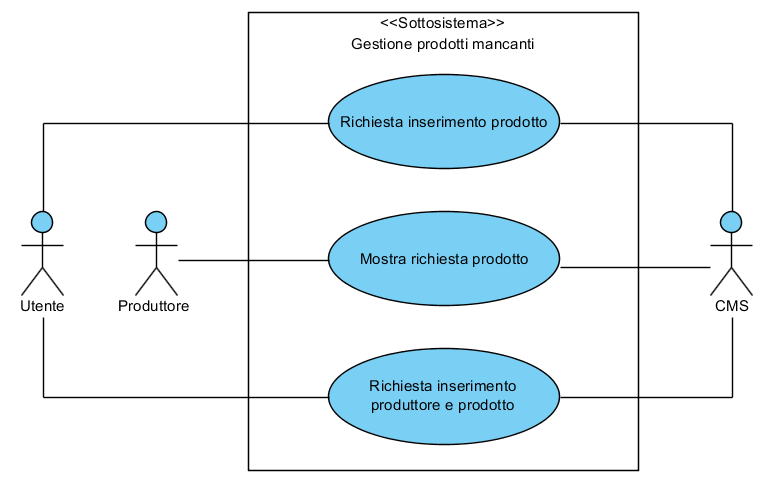
\includegraphics[width=\textwidth]{assets/visualParadigm/cu/GestioneProdottiMancanti}
\end{center}
%****************** RICHIESTA PRODOTTO ***********
\cuTab{cu:richiestaInsProdotto}
{\getTitletodesc{att:utente}}
{La persona connessa al sito è autenticata come Utente. Il sistema sta mostrando alla persona la vetrina di un Produttore}
{Il sistema contiene la richiesta di inserimento della scheda del prodotto creata, indirizzata al Produttore}
{\begin{enumCU}
		\item Il caso d'uso ha inizio quando un Utente richiede al Produttore, proprietario della vetrina che sta visualizzando, di inserire una sua scheda prodotto non già presente
		\item Il sistema richiede di compilare una scheda provvisoria del prodotto da inserire
		\item L'Utente inserisce i dati richiesti\label{curicinsimmpro:1}
		\item L'Utente conferma i dati inseriti 
		\item Il sistema richiede zero o più percorsi nel file system, o nella rete, delle immagini del prodotto da inserire
		\item L'Utente inserisce nell'apposito campo zero o più percorsi delle immagini che vuole inserire\label{curicinsimmpro:2}
		\item L'Utente conferma i percorsi inseriti\label{curicinsimmpro:3}
		\item Il sistema memorizza i dati inseriti, i percorsi inseriti e carica le immagini nel sistema
		\item Il sistema crea una nuova richiesta di inserimento prodotto per il Produttore
	\end{enumCU}}
%
\cuAlternativo{cu:richiestaInsProdotto}
{Flusso alternativo 1}%
{Annulla richiesta}%
{La persona connessa al sito è autenticata come Utente. Il sistema sta mostrando alla persona la vetrina di un Produttore}%
{\postNulle}%
{\begin{enumCU}
		\item Dopo il punto \ref{curicinsimmpro:2} o dopo il punto \ref{curicinsimmpro:1} l'Utente annulla la richiesta
	\end{enumCU}}%
%
\cuAlternativo{cu:richiestaInsProdotto}
{Flusso alternativo 2}%
{Errore richiesta}%
{La persona connessa al sito è autenticata come Utente. Il sistema sta mostrando alla persona la vetrina di un Produttore}%
{\postNulle}%
{\begin{enumCU}
		\item Dopo il punto \ref{curicinsimmpro:3} il sistema non riesce a trovare, caricare o inserire correttamente una o più immagini
	\end{enumCU}}%

\vspaceTab

\cuTab{cu:mostraRichiestaInsProdotto}
{\getTitletodesc{att:produttore}}
{La persona connessa al sito è autenticata come Produttore. Nel sistema è presente una richiesta di inserimento prodotto a lei indirizzata}
{Nella vetrina del Produttore è presente la scheda del prodotto suggerito}
{\begin{enumCU}
		\item Il caso d'uso ha inizio quando un Produttore richiedere di visualizzare le proprie richieste di aggiunta di schede prodotto in sospeso
		\item Il sistema richiede di selezionare quale richiesta visualizzare
		\item Il Produttore seleziona una richiesta
		\item Il sistema mostra al Produttore la scheda provvisoria del prodotto compilata dall'Utente che ha effettuato la richiesta \label{cuvisricprodel}
		\item Il Produttore modifica i campi nella scheda o inserisce quelli mancanti \label{cuvisricpro:1}
		\item Il Produttore conferma i dati inseriti
		\item Il sistema richiede zero o più percorsi nel file system, o nella rete, delle immagini del prodotto da inserire
		\item Il Produttore inserisce nell'apposito campo uno (zero se già inserite dall'utente) o più percorsi delle immagini che vuole inserire \label{cuvisricpro:2}
		\item Il Produttore conferma i percorsi inseriti \label{cuvisricpro:3}
		\item Il sistema memorizza i dati inseriti, i percorsi inseriti e carica le immagini nel sistema
	\end{enumCU}}
%
\cuAlternativo{cu:mostraRichiestaInsProdotto}
{Flusso alternativo 1}%
{Elimina richiesta}%
{La persona connessa al sito è autenticata come Produttore. Nel sistema è presente una richiesta di inserimento prodotto a lei indirizzata}
{Nel sistema non è più presente la richiesta}%
{\begin{enumCU}
		\item Dopo il punto \ref{cuvisricprodel} il Produttore richede di eliminare la richiesta
		\item Il sistema accetta l'operazione e rimuove la richiesta
	\end{enumCU}}%
%
\cuAlternativo{cu:mostraRichiestaInsProdotto}
{Flusso alternativo 2}%
{Annulla inserimento}%
{La persona connessa al sito è autenticata come Produttore. Nel sistema è presente una richiesta di inserimento prodotto a lei indirizzata}
{\postNulle}%
{\begin{enumCU}
		\item Dopo il punto \ref{cuvisricpro:2} o dopo il punto \ref{cuvisricpro:1} il Produttore annulla l'inserimento
	\end{enumCU}}%
%
\cuAlternativo{cu:mostraRichiestaInsProdotto}
{Flusso alternativo 3}%
{Errore inserimento}%
{La persona connessa al sito è autenticata come Produttore. Nel sistema è presente una richiesta di inserimento prodotto a lei indirizzata}
{\postNulle}%
{\begin{enumCU}
		\item Dopo il punto \ref{cuvisricpro:3} il sistema non riesce a trovare, caricare o inserire correttamente una o più immagini
	\end{enumCU}}%

\vspaceTab

\cuTab{cu:richiestaInsProduttore}
{\getTitletodesc{att:utente}}
{La persona connessa al sito è autenticata come Utente}
{Nel sistema è presente il ticket creato}
{\begin{enumCU}
		\item Il caso d'uso ha inizio quando un Utente richiede di inserire la scheda di un prodotto mancante di un Produttore non presente nel sistema
		\item Il sistema richiede di compilare una scheda provvisoria del prodotto da inserire
		\item L'Utente inserisce i dati richiesti \label{cuinsproduttore:1}
		\item L'Utente conferma i dati inseriti 
		\item Il sistema richiede zero o più percorsi nel file system, o nella rete, delle immagini del prodotto da inserire
		\item L'Utente inserisce nell'apposito campo zero o più percorsi delle immagini che vuole inserire \label{cuinsproduttore:2}
		\item L'Utente conferma i percorsi inseriti \label{cuinsproduttore:3}
		\item Il sistema memorizza i dati inseriti, i percorsi inseriti e salva le immagini nel sistema
		\item Il sistema richiede di compilare un profilo provvisorio, con almeno un nome e un recapito, del produttore
		\item L'Utente inserisce i dati richiesti \label{cuinsproduttore:0}
		\item L'Utente conferma i dati inseriti
		\item Il sistema crea un ticket allegando i riferimenti alle schede compilate
	\end{enumCU}}
%
\cuAlternativo{cu:richiestaInsProduttore}
{Flusso alternativo 1}%
{Annulla inserimento}%
{La persona connessa al sito è autenticata come Utente}%
{\postNulle}%
{\begin{enumCU}
		\item Dopo il punto \ref{cuinsproduttore:1}, il punto \ref{cuinsproduttore:2} o dopo il punto \ref{cuinsproduttore:0} l'Utente annulla l'operazione
	\end{enumCU}}%
%
\cuAlternativo{cu:richiestaInsProduttore}
{Flusso alternativo 2}%
{Errore inserimento}%
{La persona connessa al sito è autenticata come Utente}%
{\postNulle}%
{\begin{enumCU}
		\item Dopo il punto \ref{cuinsproduttore:3} il sistema non riesce a trovare, caricare o inserire correttamente una o più immagini
	\end{enumCU}}%

\subsection{Visualizzazione contenuti pubblici}
\begin{center}
   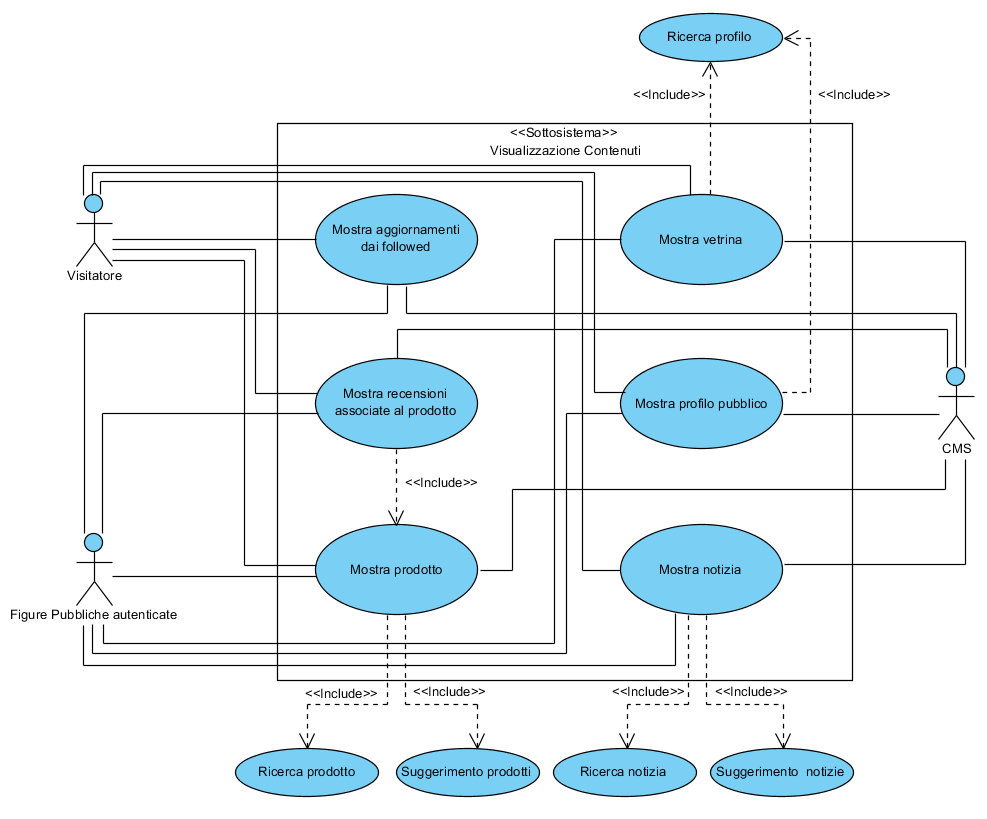
\includegraphics[width=\textwidth]{assets/visualParadigm/cu/Visualizzazione}
\end{center}
%accorpa visalizza prodotti in vetrina e visualizza vetrina
\cuTab{cu:mostraVetrina}
{\getTitletodesc{att:visitatore}, \getTitletodesc{att:figuraPubblicaAutenticata}}
{La persona è connessa al sito. Il sistema sta mostrando alla persona una lista di \glspl{anteprima} di profili di Produttori}
{Il sistema sta mostrando alla persona la vetrina del Produttore selezionato}
{\begin{enumCU}
	\item Il caso d'uso ha inizio quando una persona seleziona un \gls{anteprima} fra quelle presenti nella lista di \glspl{anteprima} di profili che sta visualizzando\label{cu:mostraVetr1}
	\item Il sistema mostra alla persona la vetrina del Produttore selezionato
\end{enumCU}
\ext{cu:statistichePrivateVetrina}
\ext{cu:personalizzaVetrinaInsProd}
\ext{cu:personalizzaVetrinaInsImg}
\ext{cu:personalizzaVetrinaDelImg}
\ext{cu:personalizzaVetrinaInsDesc}
\ext{cu:personalizzaVetrinaModDesc}
\ext{cu:richiestaInsProdotto}
}
%
\cuAlternativo{cu:mostraVetrina}%
{Flusso alternativo 1}%
{Selezione alternativa}%
{La persona è connessa al sito. Il sistema sta mostrando alla persona una lista di \glspl{anteprima} di profili}%
{Il sistema sta mostrando alla persona la vetrina selezionata}%
{\begin{enumCU}
	\item Non viene effettuato il punto \ref{cu:mostraVetr1}, ma la persona seleziona un \gls{riferimento} verso una vetrina
\end{enumCU}}%
%
\cuAlternativo{cu:mostraVetrina}%
{Flusso alternativo 2}%
{Errore ricerca}%
{La persona è connessa al sito. Il sistema sta mostrando alla persona una lista di \glspl{anteprima} di profili}%
{\postNulle}%
{\begin{enumCU}
	\item Dopo il passo \ref{cu:mostraVetr1}, non ci sono risultati per la ricerca effettuata
	\item Il sistema visualizza un avvertimento e torna al passo \ref{cu:mostraVetr1}
\end{enumCU}}%

\vspaceTab

\cuTab{cu:mostraProdotto}{\getTitletodesc{att:visitatore}, \getTitletodesc{att:figuraPubblicaAutenticata}}
{La persona è connessa al sito. Il sistema sta mostrando alla persona una lista di \glspl{anteprima} di schede di prodotti}
{Il sistema sta mostrando alla persona la scheda del prodotto selezionato}
{\begin{enumCU}
	\item Il caso d'uso ha inizio quando una persona seleziona un \gls{anteprima} fra quelle presenti nella lista di \glspl{anteprima} prodotto che sta visualizzando\label{cu:mostraProd1}
	\item Il sistema mostra alla persona il prodotto selezionato
	\item \inc{cu:suggerimentoProdotti}
\end{enumCU}
\ext{cu:personalizzaVetrinaModProd}
\ext{cu:inserisciValutazioneProdotto}
\ext{cu:modificaValutazioneProdotto}
\ext{cu:mostraRecensioniProdotto}
}
%
\cuAlternativo{cu:mostraProdotto}
{Flusso alternativo 1}%
{Selezione alternativa}%
{La persona è connessa al sito. Il sistema sta mostrando alla persona una lista di \glspl{anteprima} di schede di prodotti}%
{Il sistema sta mostrando alla persona la scheda del prodotto selezionato}%
{\begin{enumCU}
		\item Non viene effettuato il punto \ref{cu:mostraProd1}, ma la persona seleziona un \gls{riferimento} verso la scheda di un prodotto
\end{enumCU}}%
%
\cuAlternativo{cu:mostraProdotto}
{Flusso alternativo 2}%
{Errore ricerca}%
{La persona è connessa al sito. Il sistema sta mostrando alla persona una lista di \glspl{anteprima} di schede di prodotti}%
{\postNulle}%
{\begin{enumCU}
		\item Dopo il passo \ref{cu:mostraProd1}, non ci sono risultati per la ricerca effettuata
		\item Il sistema visualizza un avvertimento e torna al passo \ref{cu:mostraProd1}
\end{enumCU}}%

\vspaceTab

\cuTab{cu:mostraRecensioniProdotto}
{\getTitletodesc{att:visitatore}, \getTitletodesc{att:figuraPubblicaAutenticata}}
{La persona è connessa al sito. Il sistema sta mostrando alla persona la scheda di un prodotto}
{Il sistema sta mostrando alla persona le recensioni associate al prodotto}
{\begin{enumCU}
	\item Il caso d'uso ha inizio quando una persona richiede di visualizzare le recensioni della scheda prodotto che sta visualizzando\label{cu:mostraRec1}
	\item Il sistema mostra alla persona le recensioni relative a quel prodotto
\end{enumCU}
\ext{cu:mostraRecensione}
}
%
\cuAlternativo{cu:mostraRecensioniProdotto}
{Flusso alternativo 1}%
{Recensioni assenti}%
{La persona è connessa al sito. Il sistema sta mostrando alla persona la scheda di un prodotto}%
{\postNulle}%
{\begin{enumCU}
		\item Dopo il passo \ref{cu:mostraRec1}, non ci sono risultati per la ricerca effettuata
		\item Il sistema mostra un avvertimento e annulla l'operazione
\end{enumCU}}

\vspaceTab

\cuTab{cu:mostraRecensione}
{\getTitletodesc{att:visitatore}, \getTitletodesc{att:figuraPubblicaAutenticata}}
{La persona è connessa al sito. Il sistema sta mostrando alla persona la lista delle recensioni associate ad un prodotto}
{Il sistema sta mostrando alla persona la recensione selezionata}
{\begin{enumCU}
	\item Il caso d'uso ha inizio quando una persona richiede di visualizzare una recensione selezionandola dalla lista di recensioni che sta visualizzando\label{cu:mostraRec2}
	\item Il sistema mostra alla persona la recensione richiesta
\end{enumCU}
\ext{cu:modificaRecensioneProdotto}
\ext{cu:eliminaRecensioneProdotto}
\ext{cu:commentoRecensione}
\ext{cu:giudizioRecensione}
\ext{cu:modificaGiudizioRecensione}
}

\vspaceTab

\cuTab{cu:mostraProfilo}
{\getTitletodesc{att:visitatore}, \getTitletodesc{att:figuraPubblicaAutenticata}}
{La persona è connessa al sito. Il sistema sta mostrando alla persona una lista di \glspl{anteprima} di profili}
{Il sistema sta mostrando alla persona il profilo selezionato}
{\begin{enumCU}
	\item Il caso d'uso ha inizio quando una persona seleziona un \gls{anteprima} fra quelle presenti nella lista di \glspl{anteprima} di profili che sta visualizzando\label{cu:mostraProf1}
	\item Il sistema mostra alla persona il profilo selezionato
\end{enumCU}
\ext{cu:rimozioneAccountAltrui}
\ext{cu:modificaPrivilegiAccount}
\ext{cu:followAccount}
\ext{cu:unFollowAccount}
\ext{cu:modificaProfilo}
\ext{cu:inserisciImgProfilo}
\ext{cu:rimuoviImgProfilo}
}
%
\cuAlternativo{cu:mostraProfilo}
{Flusso alternativo 1}%
{Selezione alternativa}%
{La persona è connessa al sito. Il sistema sta mostrando alla persona una lista di \glspl{anteprima} di profili}%
{Il sistema sta mostrando alla persona il profilo}%
{\begin{enumCU}
		\item Non viene effettuato il punto \ref{cu:mostraProf1}, ma la persona seleziona un \gls{riferimento} verso un profilo
\end{enumCU}}%
%
\cuAlternativo{cu:mostraProfilo}
{Flusso alternativo 2}%
{Errore ricerca}%
{La persona è connessa al sito. Il sistema sta mostrando alla persona una lista di \glspl{anteprima} di profili}%
{\postNulle}%
{\begin{enumCU}
		\item Dopo il passo \ref{cu:mostraProf1}, non ci sono risultati per la ricerca effettuata
		\item Il sistema visualizza un avvertimento e torna al passo \ref{cu:mostraProf1}
\end{enumCU}}%

\vspaceTab

\cuTab{cu:mostraNotizia}
{\getTitletodesc{att:visitatore}, \getTitletodesc{att:figuraPubblicaAutenticata}}
{La persona è connessa al sito. Il sistema sta mostrando alla persona una lista di \glspl{anteprima} di notizie}
{Il sistema sta mostrando alla persona la notizia selezionata}
{\begin{enumCU}
	\item Il caso d'uso ha inizio quando una persona seleziona un \gls{anteprima} fra quelle presenti nella lista di \glspl{anteprima} di notizie che sta visualizzando\label{cu:mostraNot1}
	\item Il sistema mostra alla persona la notizia selezionata
	\item \inc{cu:notizieSimili}
\end{enumCU}
\ext{cu:modificaNotizia}
\ext{cu:rimozioneNotizia}
}
%
\cuAlternativo{cu:mostraNotizia}
{Flusso alternativo 1}%
{Selezione alternativa}%
{La persona è connessa al sito. Il sistema sta mostrando alla persona una lista di \glspl{anteprima} di notizie}%
{Il sistema sta mostrando alla persona la notizia scelta}%
{\begin{enumCU}
		\item Non viene effettuato il punto \ref{cu:mostraNot1}, ma la persona seleziona un \gls{riferimento} verso una notizia.
\end{enumCU}}%
%
\cuAlternativo{cu:mostraNotizia}
{Flusso alternativo 2}%
{Errore ricerca}%
{La persona è connessa al sito. Il sistema sta mostrando alla persona una lista di \glspl{anteprima} di notizie}%
{\postNulle}%
{\begin{enumCU}
		\item Dopo il passo \ref{cu:mostraNot1}, non ci sono risultati per la ricerca effettuata
		\item Il sistema visualizza un avvertimento e torna al passo \ref{cu:mostraNot1}
\end{enumCU}}%

\vspaceTab

\cuTab{cu:mostraAggF}
{\getTitletodesc{att:figuraPubblicaAutenticata}}
{La persona è connessa al sito ed ha i privilegi di Figura Pubblica Autenticata}
{Il sistema sta mostrando alla persona la pagina degli aggiornamenti dai followed}
{\begin{enumCU}
	\item Il caso d'uso ha inizio quando una persona richiede di visualizzare gli aggiornamenti delle persone che segue
	\item Il sistema mostra alla persona gli aggiornamenti delle persone che segue
\end{enumCU}}

\begin{landscape}
\section{Matrice di tracciabilità}
\begin{center}
	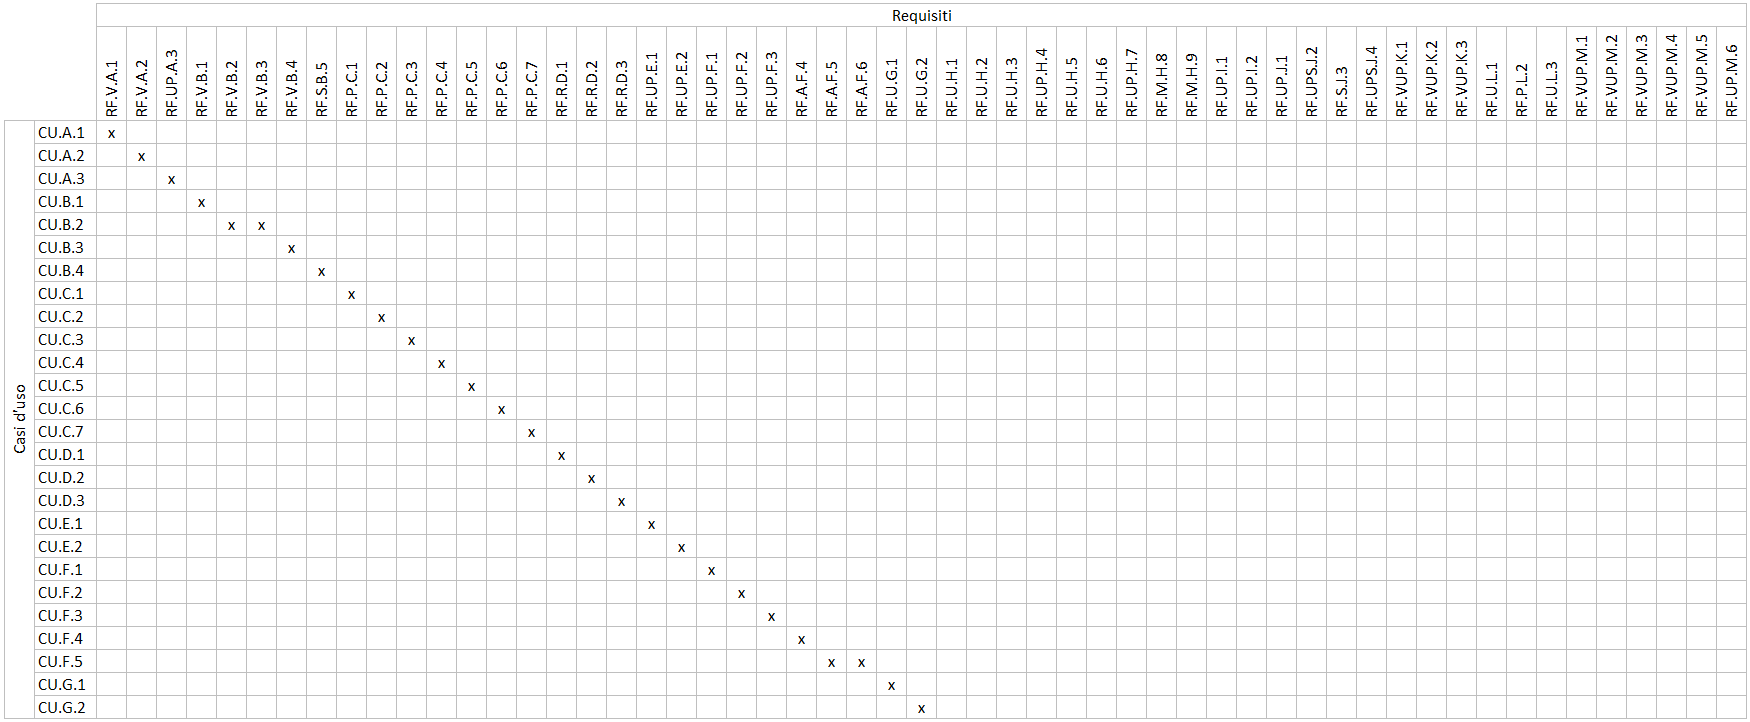
\includegraphics[width=\linewidth]{assets/matricetracciabilita0}
\end{center}
\end{landscape}

\begin{landscape}
\begin{center}
	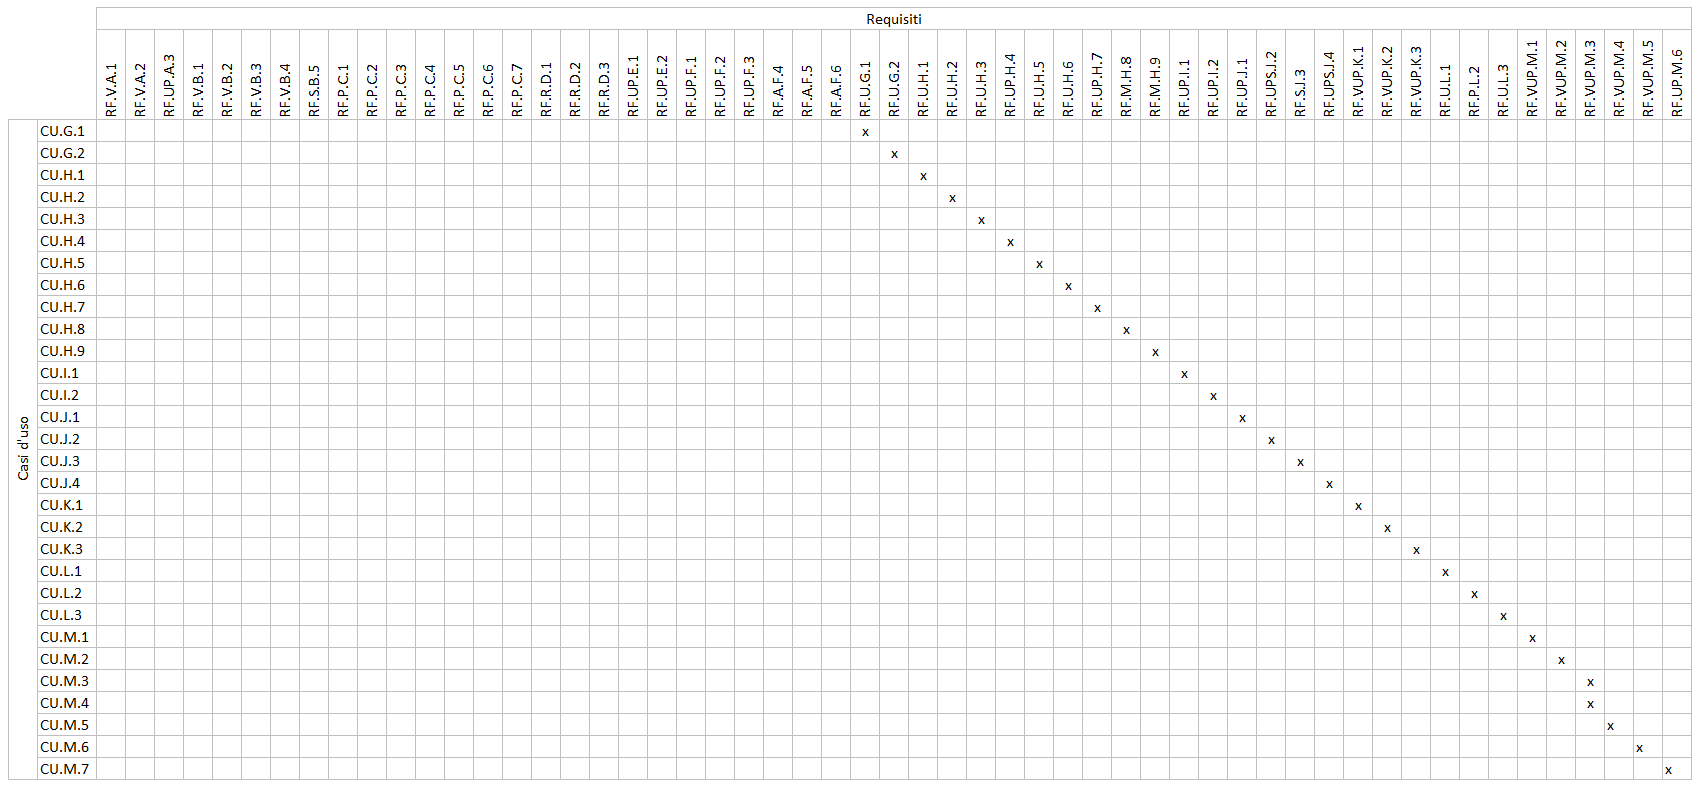
\includegraphics[width=\linewidth]{assets/matricetracciabilita1}
\end{center}
\end{landscape}

\newdate{cuuno}{12}{09}{2016}
\newdate{cudue}{29}{09}{2016}
\section{Revisioni}
\begin{center}
    \begin{tabular}{lll}
        \toprule
        	\tabhead{Versione} & \tabhead{Data} & \tabhead{Descrizione} \\
		\cmidrule(l{\cmidrulekern}r{\cmidrulekern}){1-3}
        	1.0 & \displaydate{cuuno} & Prima versione \\
        	1.1 & \displaydate{cudue} & Riorganizzati casi d'uso \\
        \bottomrule
    \end{tabular}
\end{center}
    \chapter{Valutazione dei rischi} 

\section{Introduzione}
In questo documento verrà effettuata l'analisi dei rischi, per gestire eventuali imprevisti e limitarne i danni, i quali comporterebbero possibili aumenti del costo, ritardi rispetto alla \docref{cha:pianificazione_del_progetto} o, nei casi più gravi, l'annullamento dell'intero progetto.

Compileremo delle tabelle con alcuni dei possibili rischi, in cui verrà indicata la probabilità del rischio e la tipologia dell'effetto negaativo che il rischio comporta. I rischi più probabili e quelli con i maggiori effetti negativi dovranno essere oggetto di maggiori attenzioni durante lo sviluppo del progetto.

\section{Classificazione probabilità}
Le probabilità del verificarsi di un rischio vengono, per semplicità, così classificate:
\begin{center}
	\begin{tabularx}{\widthTab}{ l  X } 
		\toprule
			\formattaTitoloTab{Classificazione} & \formattaTitoloTab{Probabilità} \\
		\cmidrule(l{\cmidrulekern}r{\cmidrulekern}){1-2}
			Molta alta & maggiore del 75\% \\ 
			\addlinespace[1em] 
			Alta & compresa fra il 50\% e il 75\%  \\ 
			\addlinespace[1em] 
			Meida & compresa fra il 25\% e il 50\%  \\ 
			\addlinespace[1em] 
			Bassa & compresa fra il 10\% e il 25\%  \\ 
			\addlinespace[1em] 
			Molto bassa & minore del 10\% \\ 
		\bottomrule
	\end{tabularx}
\end{center}

\section{Classificazione effetti}
I possibili eventi che un rischio può provocare vengono così suddivisi:
\begin{center}
	\begin{tabularx}{\widthTab}{ l  X } 
		\toprule
			\formattaTitoloTab{Classificazione} & \formattaTitoloTab{Effetti} \\
		\cmidrule(l{\cmidrulekern}r{\cmidrulekern}){1-2}
			Catastrofici & Il verificarsi del rischio probabilmente comporta il fallimento del progetto \\ 
			\addlinespace[1em] 
			Seri & Il verificarsi del rischio, se non correttamente gestito, potrebbe comportare il fallimento del progetto o ad ingenti aumenti di costo e del tempo richiesto per il completamento dello stesso \\ 
			\addlinespace[1em] 
			Tollerabili & Il verificarsi del rischio comporta un aumento dei costi e un ritardo nel completamento del progetto  \\ 
			\addlinespace[1em] 
			Insignificanti & Il verificarsi del rischio non comporta aumenti di costo o ritardi \\
		\bottomrule
	\end{tabularx}
\end{center}

\section{Elenco dei rischi}
Vengono di seguito elencati i possibili rischi che possono verificarsi:
\begin{itemize}
	\item \newListItem{rk:ritardo}{\formattaRK}{Ritardi}
	\item \newListItem{rk:reqerrati}{\formattaRK}{Requisiti errati}
	\item \newListItem{rk:reqincompleti}{\formattaRK}{Requisiti incompleti}
	\item \newListItem{rk:reqcambiati}{\formattaRK}{Requisiti cambiati}
	\item \newListItem{rk:ucerrati}{\formattaRK}{Use Case errati}
	\item \newListItem{rk:ucincompleti}{\formattaRK}{Use Case incompleti}
	\item \newListItem{rk:docerrata}{\formattaRK}{Documentazione incompleta o errata}
	\item \newListItem{rk:complessita}{\formattaRK}{Complessità sottovalutata}
\end{itemize}

\section{Specifica tabelle RMMM}
Le tabelle del \gls{rmmm} servono per gestire i rischi, la loro specifica indica tre diverse fasi per ogni rischio:
\begin{descriptionInd}
	\item[Mitigation] Come cercare di impedire il verificarsi del rischio adottando alcune tecniche o strategie
	\item[Monitoring] Come sorvegliare il lavoro progettuale per accorgersi del rischio in tempo utile
	\item[Management] Come gestire il rischio nel caso esso si verifichi
\end{descriptionInd}
Di seguito elenchiamo le tabelle \gls{rmmm}:

\rkTab{rk:ritardo}{}{}{}{}{}{}
\rkTab{rk:reqerrati}{}{}{}{}{}{}
\rkTab{rk:reqincompleti}{}{}{}{}{}{}
\rkTab{rk:reqcambiati}{}{}{}{}{}{}
\rkTab{rk:ucerrati}{}{}{}{}{}{}
\rkTab{rk:ucincompleti}{}{}{}{}{}{}
\rkTab{rk:docerrata}{}{}{}{}{}{}
\rkTab{rk:complessita}{}{}{}{}{}{}

    \chapter{Stima dei costi}

\section{Introduzione}
In questo documento utilizzeremo il metodo \gls{ucp} per calcolare la stima della dimensione del progetto. Tale metodo si basa sul calcolo dei seguenti elementi:
\begin{itemize}
	\item \gls{uaw} una stima che tiene del numero e della complessità degli attori
	\item \gls{uucw} una stima che tiene del numero e della complessità dei casi d'uso
	\item \gls{tcf} un fattore che è usato per aggiustare la stima basandosi su considerazioni tecniche
	\item \gls{ecf} un fattore che è usato per aggiustare la stima basandosi su considerazioni ambientali
\end{itemize}

\section{Stima della complessità degli attori}
Gli attori vengono classificati in una scala di tre valori, in base alla loro complessità. Il metodo \gls{ucp} definisce le seguenti direttive per catalogare gli attori:
\begin{center}
	\begin{tabularx}{\widthTab}{ l  X  l} 
		\toprule
			\formattaTitoloTab{Classificazione} & \formattaTitoloTab{Tipo di attore} & \formattaTitoloTab{Peso} \\
		\cmidrule(l{\cmidrulekern}r{\cmidrulekern}){1-3}
			\formattaCampiTab{Simple} & L'attore è un sistema esterno che utilizza una \gls{api} & 1 \\ 
			\addlinespace[1em] 
			\formattaCampiTab{Average} & L'attore è un sistema esterno che utilizza un protocollo (ad esempio TCP/IP, FTP, HTTP) & 2 \\ 
			\addlinespace[1em] 
			\formattaCampiTab{Complex} & L'attore è un utente che utilizza una \gls{gui} & 3 \\ 
		\bottomrule
	\end{tabularx}
\end{center}
La stima del costo degli attori (\gls{uaw}) è data dalla seguente formula:
\begin{displaymath}
UAW = (NoSimpleActors \times 1) + (NoAvgActors \times 2) + (NoComplexActors \times 3)
\end{displaymath}
Di seguito riportiamo la tabella con indicati pesi di ogni attore:
\begin{center}
	\begin{tabularx}{\widthTab}{ l  X  l} 
		\toprule
			\formattaTitoloTab{ID} & \formattaTitoloTab{Attore} & \formattaTitoloTab{Peso} \\
		\cmidrule(l{\cmidrulekern}r{\cmidrulekern}){1-3}
			\rowIDTitle{att:visitatore} & 3 \\ 
			\addlinespace[1em] 
			\rowIDTitle{att:figuraPubblicaAutenticata} & 3 \\ 
			\addlinespace[1em] 
			\rowIDTitle{att:figuraAmministrativa} & 3 \\ 
			\addlinespace[1em] 
			\rowIDTitle{att:utente} & 3 \\ 
			\addlinespace[1em] 
			\rowIDTitle{att:produttore} & 3 \\ 
			\addlinespace[1em] 
			\rowIDTitle{att:redattore} & 3 \\ 
			\addlinespace[1em] 
			\rowIDTitle{att:assistente} & 3 \\ 
			\addlinespace[1em] 
			\rowIDTitle{att:moderatore} & 3 \\ 
			\addlinespace[1em] 
			\rowIDTitle{att:amministratore} & 3 \\ 
			\addlinespace[1em] 
			\rowIDTitle{att:cms} & 2 \\ 
		\cmidrule(l{\cmidrulekern}r{\cmidrulekern}){1-3}
			\formattaCampiTab{\gls{uaw}}  & & 29\\
		\bottomrule
	\end{tabularx}
\end{center}

\section{Stima della complessità dei casi d'uso}
I casi d'uso vengono classificati in una scala di tre valori, in base alla loro complessità. Il metodo \gls{ucp} definisce le seguenti direttive per catalogare i casi d'uso:
\begin{center}
	\begin{tabularx}{\widthTab}{ l  X  l} 
		\toprule
			\formattaTitoloTab{Classificazione} & \formattaTitoloTab{Numero di transazioni} & \formattaTitoloTab{Peso} \\
		\cmidrule(l{\cmidrulekern}r{\cmidrulekern}){1-3}
			\formattaCampiTab{Simple} & Un numero di transazioni compreso fra 1 e 3 & 5 \\ 
			\addlinespace[1em] 
			\formattaCampiTab{Average} & Un numero di transazioni compreso fra 4 e 7 & 10 \\ 
			\addlinespace[1em] 
			\formattaCampiTab{Complex} & Un numero di transazioni pari a 8 o maggiore & 15 \\ 
		\bottomrule
	\end{tabularx}
\end{center}
La stima del costo dei casi d'uso (\gls{uucw}) è data dalla seguente formula:
\begin{displaymath}
UUCW = (NoSimpleUC \times 5) + (NoAvgUC \times 10) + (NoComplexUC \times 15)
\end{displaymath}
Di seguito riportiamo la tabella con indicati pesi di ogni attore: 
\begin{center}
	\begin{longtable}{ p{0.125\textwidth} p{0.7\textwidth} p{0.075\textwidth} } 
		\toprule
			\formattaTitoloTab{ID} & \formattaTitoloTab{Caso d'uso} & \formattaTitoloTab{Peso} \\
		\cmidrule(l{\cmidrulekern}r{\cmidrulekern}){1-3}
		\endfirsthead

		\toprule
			\formattaTitoloTab{ID} & \formattaTitoloTab{Attore} & \formattaTitoloTab{Peso} \\
		\cmidrule(l{\cmidrulekern}r{\cmidrulekern}){1-3}
		\endhead

		\midrule
		\multicolumn{3}{r}{\footnotesize\itshape continua nella prossima pagina} \\
		\endfoot

		\bottomrule
		\endlastfoot

			\rowIDTitle{cu:login} & 5 \\ 
			\addlinespace[1em] 
			\rowIDTitle{cu:loginAmm} & 5 \\ 
			\addlinespace[1em] 
			\rowIDTitle{cu:logout} & 5 \\ 
			\addlinespace[1em] 
			\rowIDTitle{cu:iscrizionePortale} & 5 \\ 
			\addlinespace[1em] 
			\rowIDTitle{cu:iscrizioneSocial} & 5 \\ 
			\addlinespace[1em] 
			\rowIDTitle{cu:iscrizioneApprovazione} & 5 \\ 
			\addlinespace[1em] 
			\rowIDTitle{cu:approvazioneIscrizione} & 5 \\ 
			\addlinespace[1em] 
			\rowIDTitle{cu:personalizzaVetrinaInsDesc} & 5 \\ 
			\addlinespace[1em] 
			\rowIDTitle{cu:personalizzaVetrinaModDesc} & 5 \\ 
			\addlinespace[1em] 
			\rowIDTitle{cu:personalizzaVetrinaInsImg} & 5 \\ 			
			\addlinespace[1em] 
			\rowIDTitle{cu:personalizzaVetrinaDelImg} & 5 \\ 
			\addlinespace[1em] 
			\rowIDTitle{cu:personalizzaVetrinaInsProd} & 5 \\ 
			\addlinespace[1em] 
			\rowIDTitle{cu:personalizzaVetrinaModProd} & 5 \\ 
			\addlinespace[1em] 
			\rowIDTitle{cu:statistichePrivateVetrina} & 5 \\ 
			\addlinespace[1em] 
			\rowIDTitle{cu:inserimentoNotizia} & 5 \\ 
			\addlinespace[1em] 
			\rowIDTitle{cu:modificaNotizia} & 5 \\ 
			\addlinespace[1em] 
			\rowIDTitle{cu:rimozioneNotizia} & 5 \\ 
			\addlinespace[1em] 
			\rowIDTitle{cu:suggerimentoProdotti} & 5 \\ 
			\addlinespace[1em] 
			\rowIDTitle{cu:notizieSimili} & 5 \\ 
			\addlinespace[1em] 
			\rowIDTitle{cu:modificaProfilo} & 5 \\ 
			\addlinespace[1em]
			\rowIDTitle{cu:inserisciImgProfilo} & 5 \\ 
			\addlinespace[1em]  
			\rowIDTitle{cu:rimuoviImgProfilo} & 5 \\ 
			\addlinespace[1em] 
			\rowIDTitle{cu:modificaImpostazioni} & 5 \\ 
			\addlinespace[1em] 
			\rowIDTitle{cu:rimozioneAccountProprio} & 5 \\ 
			\addlinespace[1em] 
			\rowIDTitle{cu:rimozioneAccountAltrui} & 5 \\ 
			\addlinespace[1em] 
			\rowIDTitle{cu:modificaPrivilegiAccount} & 5 \\ 
			\addlinespace[1em] 
			\rowIDTitle{cu:inserisciValutazioneProdotto} & 5 \\ 
			\addlinespace[1em] 
			\rowIDTitle{cu:modificaValutazioneProdotto} & 5 \\ 
			\addlinespace[1em] 
			\rowIDTitle{cu:inserisciRecensioneProdotto} & 5 \\ 
			\addlinespace[1em] 
			\rowIDTitle{cu:modificaRecensioneProdotto} & 5 \\ 			
			\addlinespace[1em] 
			\rowIDTitle{cu:eliminaRecensioneProdotto} & 5 \\ 
			\addlinespace[1em] 
			\rowIDTitle{cu:commentoRecensione} & 5 \\ 
			\addlinespace[1em] 
			\rowIDTitle{cu:giudizioRecensione} & 5 \\ 
			\addlinespace[1em] 
			\rowIDTitle{cu:modificaGiudizioRecensione} & 5 \\ 
			\addlinespace[1em] 
			\rowIDTitle{cu:segnalazioneContenutiInap} & 5 \\ 
			\addlinespace[1em] 
			\rowIDTitle{cu:mostraSegnContenutiInap} & 5 \\ 
			\addlinespace[1em] 
			\rowIDTitle{cu:rimozioneContenutiInap} & 5 \\ 
			\addlinespace[1em] 
			\rowIDTitle{cu:followAccount} & 5 \\ 
			\addlinespace[1em] 
			\rowIDTitle{cu:unFollowAccount} & 5 \\ 
			\addlinespace[1em] 
			\rowIDTitle{cu:ticketInvio} & 5 \\ 
			\addlinespace[1em] 
			\rowIDTitle{cu:ticketRisposta} & 5 \\ 
			\addlinespace[1em] 
			\rowIDTitle{cu:ticketChiudi} & 5 \\ 
			\addlinespace[1em] 
			\rowIDTitle{cu:ticketLettura} & 5 \\ 
			\addlinespace[1em] 
			\rowIDTitle{cu:ricercaProdotto} & 5 \\ 
			\addlinespace[1em] 
			\rowIDTitle{cu:ricercaProfilo} & 5 \\ 
			\addlinespace[1em] 
			\rowIDTitle{cu:ricercaNotizia} & 5 \\ 
			\addlinespace[1em] 
			\rowIDTitle{cu:richiestaInsProdotto} & 5 \\ 
			\addlinespace[1em] 
			\rowIDTitle{cu:mostraRichiestaInsProdotto} & 10 \\ 			
			\addlinespace[1em] 
			\rowIDTitle{cu:richiestaInsProduttore} & 10 \\ 
			\addlinespace[1em] 
			\rowIDTitle{cu:mostraVetrina} & 5 \\ 
			\addlinespace[1em] 
			\rowIDTitle{cu:mostraProdotto} & 5 \\ 
			\addlinespace[1em] 
			\rowIDTitle{cu:mostraRecensioniProdotto} & 5 \\ 
			\addlinespace[1em] 
			\rowIDTitle{cu:mostraRecensione} & 5 \\ 
			\addlinespace[1em]
			\rowIDTitle{cu:mostraProfilo} & 5 \\ 
			\addlinespace[1em] 
			\rowIDTitle{cu:mostraNotizia} & 5 \\ 
			\addlinespace[1em] 
			\rowIDTitle{cu:mostraAggF} & 5 \\ 
		\cmidrule(l{\cmidrulekern}r{\cmidrulekern}){1-3}
			\formattaCampiTab{\gls{uucw}}  & & 290\\
	\end{longtable}
\end{center}

\section{Fattore di aggiustamento tecnico}
Il \gls{tcf} è uno dei fattori che viene applicato alla stima della dimensione del progetto in modo tale da tener conto delle considerazioni tecniche.
Questo fattore è determinato assegnando un valore compreso fra 0 (irrilevante) e 5 (essenziale) ai 13 aspetti tecnici, ad ognuno dei quali è associato un peso. 
Il \gls{tcf} è dato dalla seguente formula:
\begin{displaymath}
	TCF = 0.6 + (TF \div 100)
\end{displaymath}
Dove il \gls{tf} viene così calcolato:
\begin{displaymath}
	TF = \sum_{i=1}^{13}FactorWeight_i \times FactorScore_i 
\end{displaymath}
Nella seguente tabella riportiamo gli aspetti tecnici che vengono presi in considerazione nel calcolo del \gls{tcf}, il peso di ognuno di essi e il valore che gli viene assegnato:
\begin{center}
	\begin{tabularx}{\widthTab}{l X l l} 
		\toprule
			\formattaTitoloTab{Fattore} & \formattaTitoloTab{Descrizione} & \formattaTitoloTab{Peso} & \formattaTitoloTab{Valore} \\
		\cmidrule(l{\cmidrulekern}r{\cmidrulekern}){1-4}
			\formattaCampiTab{T1} & Distributed system & 2.0 & 0.0\\ 
			\addlinespace[1em] 
			\formattaCampiTab{T2} & Response time/performance objectives & 1.0 & 5.0\\ 
			\addlinespace[1em] 
			\formattaCampiTab{T3} & End-user efficiency & 1.0 & 5.0\\ 
			\addlinespace[1em] 
			\formattaCampiTab{T4} & Internal processing complexity & 1.0 & 1.0\\ 
			\addlinespace[1em] 
			\formattaCampiTab{T5} & Code reusability & 1.0 & 3.0\\ 
			\addlinespace[1em] 
			\formattaCampiTab{T6} & Easy to install & 0.5 & 1.0\\ 
			\addlinespace[1em] 
			\formattaCampiTab{T7} & Easy to use & 0.5 & 5.0\\ 
			\addlinespace[1em] 
			\formattaCampiTab{T8} & Portability to other platforms & 2.0 & 5.0\\ 
			\addlinespace[1em] 
			\formattaCampiTab{T9} & System maintenance & 1.0 & 3.0 \\ 
			\addlinespace[1em] 
			\formattaCampiTab{T10} & Concurrent/parallel processing & 1.0 & 1.0 \\ 
			\addlinespace[1em] 
			\formattaCampiTab{T11} & Security features & 1.0 & 4.0 \\ 
			\addlinespace[1em] 
			\formattaCampiTab{T12} & Access for third parties & 1.0 & 0.0 \\ 
			\addlinespace[1em] 
			\formattaCampiTab{T13} & End user training & 1.0 & 0.0 \\ 
		\cmidrule(l{\cmidrulekern}r{\cmidrulekern}){1-4}
			\formattaCampiTab{TF} & & & 35.0 \\ 
			\formattaCampiTab{TCF} & & & 0.95 \\ 
		\bottomrule
	\end{tabularx}
\end{center}

\section{Fattore di aggiustamento ambientale}
Il \gls{ecf} è l'altro fattore che viene applicato alla stima della dimensione del progetto in modo tale da tener conto delle considerazioni ambientali.
Questo fattore è determinato assegnando un valore compreso fra 0 (nessuna esperienza) e 5 (esperto) agli 8 aspetti ambientali, ad ognuno dei quali è associato un peso. 
Il \gls{ecf} è dato dalla seguente formula:
\begin{displaymath}
	ECF = 1.4 + (-0.03 \times EF)
\end{displaymath}
Dove il \gls{ef} viene così calcolato:
\begin{displaymath}
	EF = \sum_{i=1}^{8}FactorWeight_i \times FactorScore_i 
\end{displaymath}
Nella seguente tabella riportiamo gli aspetti ambientali che vengono presi in considerazione nel calcolo del \gls{ecf}, il peso di ognuno di essi e il valore che gli viene assegnato:
\begin{center}
	\begin{tabularx}{\widthTab}{l X l l} 
		\toprule
			\formattaTitoloTab{Fattore} & \formattaTitoloTab{Descrizione} & \formattaTitoloTab{Peso} & \formattaTitoloTab{Valore} \\
		\cmidrule(l{\cmidrulekern}r{\cmidrulekern}){1-4}
			\formattaCampiTab{E1} & Familiarity with development process used & 1.5 & 0.5\\ 
			\addlinespace[1em] 
			\formattaCampiTab{E2} & Application experience & 0.5 & 0.0\\ 
			\addlinespace[1em] 
			\formattaCampiTab{E3} & Object-oriented experience of team & 1.0 & 5.0\\ 
			\addlinespace[1em] 
			\formattaCampiTab{E4} & Lead analyst capability & 0.5 & 2.5\\ 
			\addlinespace[1em] 
			\formattaCampiTab{E5} & Motivation of the team & 1.0 & 5.0\\ 
			\addlinespace[1em] 
			\formattaCampiTab{E6} & Stability of requirements & 2.0 & 3.0\\ 
			\addlinespace[1em] 
			\formattaCampiTab{E7} & Part-time staff & -1.0 & 0.0\\ 
			\addlinespace[1em] 
			\formattaCampiTab{E8} & Difficult programming language & -1.0 & 2.0\\ 
		\cmidrule(l{\cmidrulekern}r{\cmidrulekern}){1-4}
			\formattaCampiTab{EF} & & & 16.0 \\ 
			\formattaCampiTab{ECF} & & & 0.92 \\ 
		\bottomrule
	\end{tabularx}
\end{center}

\section{Calcolo UCP}
Il valore finale degli \acrfull{ucp} è dato dalla seguente formula:
\begin{displaymath}
	UCP = (UAW + UUCW) \times TCF \times ECF = (29 + 290) \times 0.95 \times 0.92 = 278.806 
\end{displaymath}

\section{Stima dello sforzo}
Una volta nota la stima della dimensione del progetto è possibile stimare lo sforzo necessario per comopletarlo.
Si assume, non avendo esperienze passate, che per ogni \gls{ucp} siano necessarie 30 ore/uomo.
Lo sforzo totale per il completamento del progetto, \gls{ee}, è dato dalla seguente formula:
\begin{displaymath}
	EE = UCP \times (Hours Per UCP) = 278.806 \times 30 = 8364.18\, ore/uomo
\end{displaymath}
In un giorno si hanno generalmente 8 ore lavorative, quindi, dividendo la quantità precedente per 8 si ottiene lo sforzo in giorni/uomo:
\begin{displaymath}
	EE = 8364.18 \div 8 = 1045.52\, giorni/uomo
\end{displaymath}
In un mese si hanno generalmente 22 giorni lavorativi, quindi, dividendo la quantità precedente per 22 si ottiene lo sforzo in mesi/uomo:
\begin{displaymath}
	EE = 1045.52 \div 22 = 47.52\, mesi/uomo
\end{displaymath}
Quindi lo sforzo in anni/uomo è il seguente:
\begin{displaymath}
	EE = 47.52 \div 12 = 3.96\, anni/uomo
\end{displaymath}
Con un team di tre persone si stima il completamento del progetto entro 2 anni.

\section{Stima del costo}
Supponendo uno stipendio medio di \(4000\, euro\) si stima il seguente costo del progetto:
\begin{displaymath}
	COSTO = 47.52 \times 4000 = 190080\, euro
\end{displaymath}

\newdate{costiuno}{03}{10}{2016}
\newdate{seconda}{06}{10}{2016}
\section{Revisioni}
\begin{center}
    \begin{tabular}{lll}
        \toprule
        	\tabhead{Versione} & \tabhead{Data} & \tabhead{Descrizione} \\
		\cmidrule(l{\cmidrulekern}r{\cmidrulekern}){1-3}
        	1.0 & \displaydate{costiuno} & Prima versione \\
        	1.1 & \displaydate{seconda} & Aggiornati i pesi dei casi d'uso, lo sforzo e il costo \\
        \bottomrule
    \end{tabular}
\end{center}   
    \chapter{Analisi del sistema}

\section{Introduzione}
In questo documento effetturemo l'analisi del sistema, ci avvarremo del linguaggio \gls{uml} per formalizzare i requisiti descritti nel documento \docref{cha:specifica_requisiti} e in parte espressi nei casi d'uso nella \docref{cha:usecase}.
Effettueremo la formalizzazione esclusivamente delle parti prinicpali del sistema, in particolare andremo a realizzare i seguenti diagrammi:
\begin{itemize}
	\item Diagrammi di attività
	\item Diagramma dei package
	\item Diagrammi delle classi
	\item Diagrammi di sequenza
\end{itemize}

\section{Diagrammi di attività}
I diagrammi di attività descrivono il comportamento nel tempo di un particolare elemento. Con essi si modella l’interazione e la fusione dei flussi principali con i flussi alternativi dei casi d’uso. Questo viene fatto per rendere più visibili le varie ramificazioni che i flussi possono avere all’interno di un caso d’uso. Non verranno rappresentati tutti i diagrammi di attività, ma solo quelli corrispondenti ai casi d'uso principali.
\begin{center}
	\begin{tabularx}{\textwidth}{ l X } 
		\toprule
		\formattaTitoloTab{ID} & \formattaTitoloTab{Caso d'uso di riferimento} \\
		\cmidrule(l{\cmidrulekern}r{\cmidrulekern}){1-2}
		\newAttivita{da:login}{\formattaAT}{Login} & \getIDTitletodesc{cu:login} \\ 
		\addlinespace[1em] 
		\newAttivita{da:logout}{\formattaAT}{Logout} & \getIDTitletodesc{cu:logout} \\ 
		\addlinespace[1em] 
		\newAttivita{da:iscrizione}{\formattaAT}{Iscrizione} & \getIDTitletodesc{cu:iscrizionePortale} \\
		 													 & \getIDTitletodesc{cu:iscrizioneSocial} \\
															 & \getIDTitletodesc{cu:iscrizioneApprovazione} \\ 
		\addlinespace[1em] 
		\newAttivita{da:approvazione}{\formattaAT}{Approvazione iscrizione} & \getIDTitletodesc{cu:approvazioneIscrizione} \\ 
		\addlinespace[1em]
		\newAttivita{da:schedaprodotto}{\formattaAT}{Inserimento scheda prodotto} & \getIDTitletodesc{cu:personalizzaVetrinaInsProd} \\
		\addlinespace[1em]
		\newAttivita{da:ricerche}{\formattaAT}{Ricerche} & \getIDTitletodesc{cu:ricercaProdotto} \\
														 & \getIDTitletodesc{cu:ricercaNotizia} \\
														 & \getIDTitletodesc{cu:ricercaProfilo} \\
		\addlinespace[1em]
		\newAttivita{da:valrec}{\formattaAT}{Inserimento valutazione e recensione} & \getIDTitletodesc{cu:inserisciValutazioneProdotto} \\
																				   & \getIDTitletodesc{cu:inserisciRecensioneProdotto}\\
		\addlinespace[1em]
		\newAttivita{da:oprec}{\formattaAT}{Operazioni recensione} & \getIDTitletodesc{cu:modificaRecensioneProdotto}\\
																   & \getIDTitletodesc{cu:eliminaRecensioneProdotto}\\
																   & \getIDTitletodesc{cu:commentoRecensione}\\
																   & \getIDTitletodesc{cu:giudizioRecensione}\\ 
																   & \getIDTitletodesc{cu:modificaGiudizioRecensione}\\ 
		\bottomrule
	\end{tabularx}
\end{center}

\linkedSubsection{da:login}
\begin{center}
			\includegraphics[width=\textwidth]{assets/visualParadigm/attivita/login}
\end{center}

\linkedSubsection{da:logout}
\begin{center}
	\includegraphics[width=\textwidth]{assets/visualParadigm/attivita/logout}
\end{center}

\linkedSubsection{da:iscrizione}
\begin{center}
	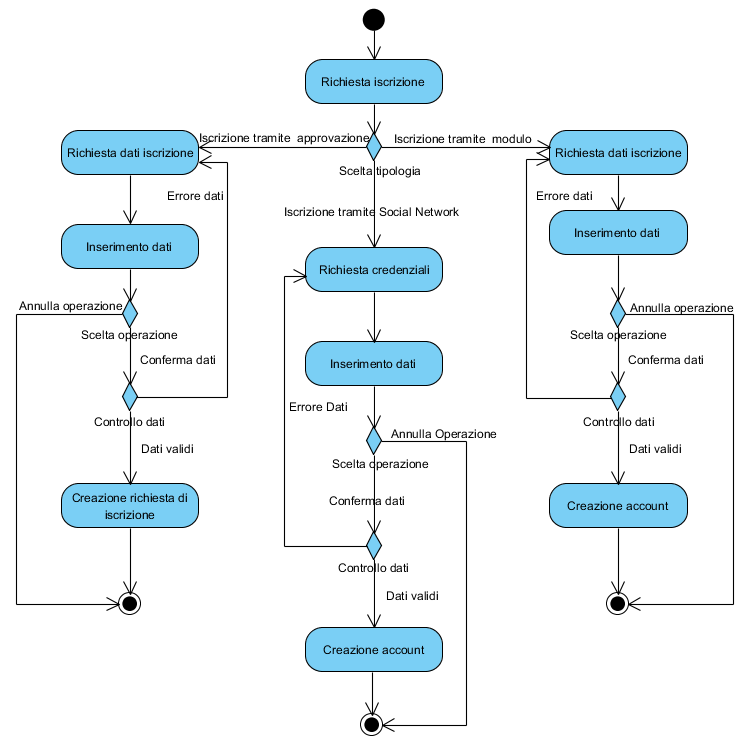
\includegraphics[width=\textwidth]{assets/visualParadigm/attivita/iscrizioni}
\end{center}

\linkedSubsection{da:approvazione}
\begin{center}
	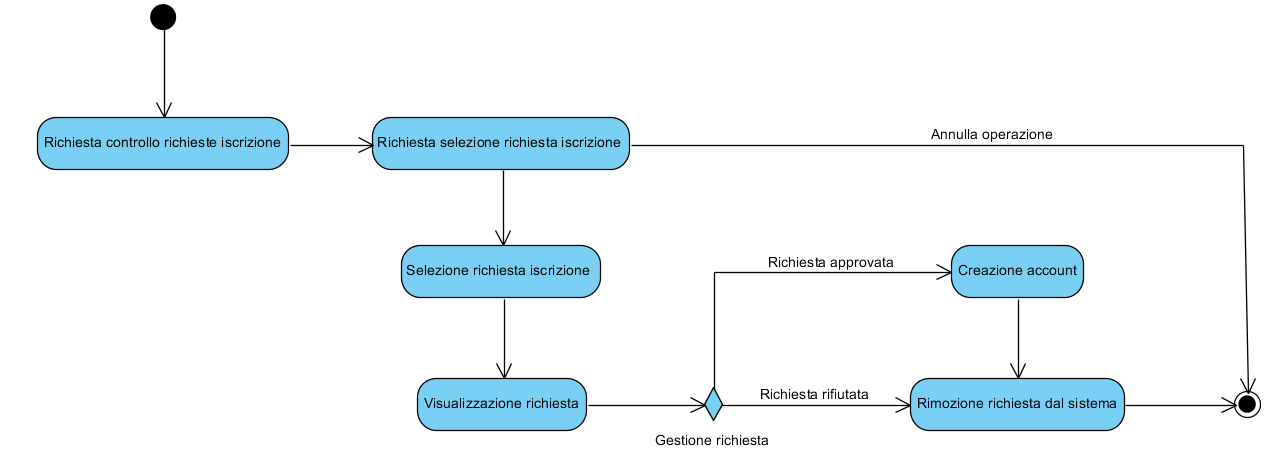
\includegraphics[width=\textwidth]{assets/visualParadigm/attivita/approvazioneIscrizione}
\end{center}

\linkedSubsection{da:schedaprodotto}
\begin{center}
	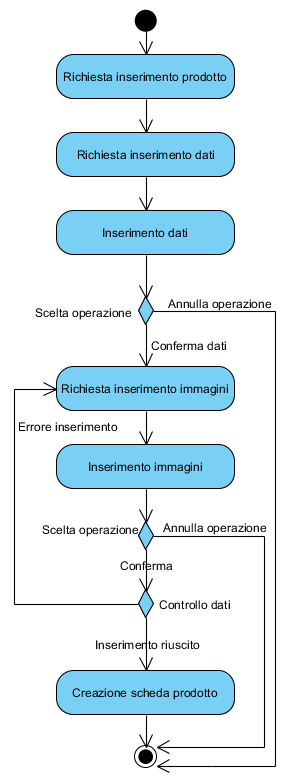
\includegraphics[width=0.5\textwidth]{assets/visualParadigm/attivita/schedaprodotto}
\end{center}

\linkedSubsection{da:ricerche}
\begin{center}
	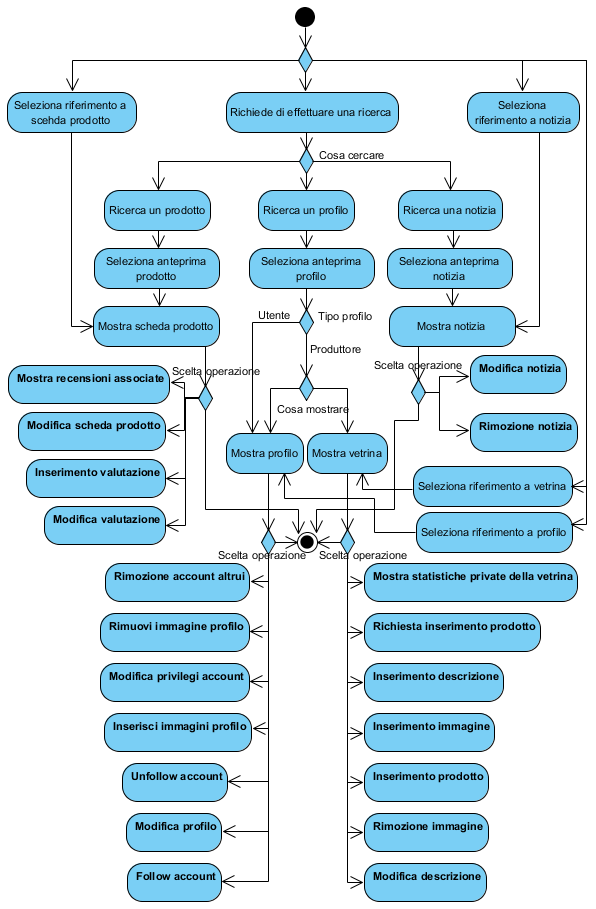
\includegraphics[width=0.95\textwidth]{assets/visualParadigm/attivita/ricerche}
\end{center}

\linkedSubsection{da:valrec}
\begin{center}
	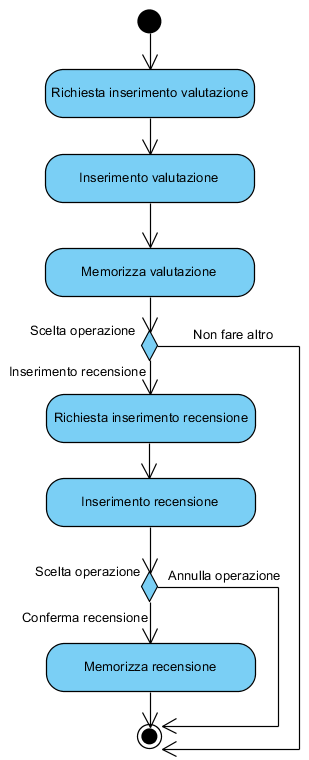
\includegraphics[width=0.5\textwidth]{assets/visualParadigm/attivita/valutazioneRecensione}
\end{center}

\linkedSubsection{da:oprec}
\begin{center}
	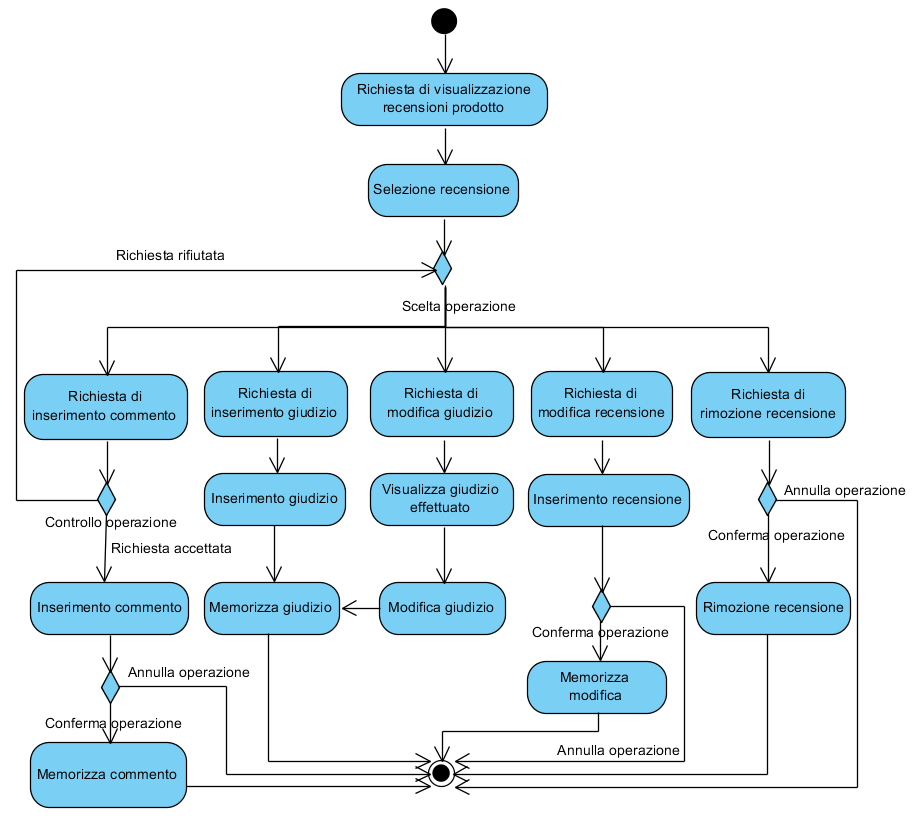
\includegraphics[width=\textwidth]{assets/visualParadigm/attivita/mostraRecensioni}
\end{center}

\begin{landscape}
\section{Diagramma dei package}
Il diagramma dei package sono diagrammi di struttura che descrive i package del sistema e le relazioni tra essi.
Un Package è uno spazio dei nomi utilizzato per raggruppare elementi che sono in relazione semantica tra loro.
\begin{center}
			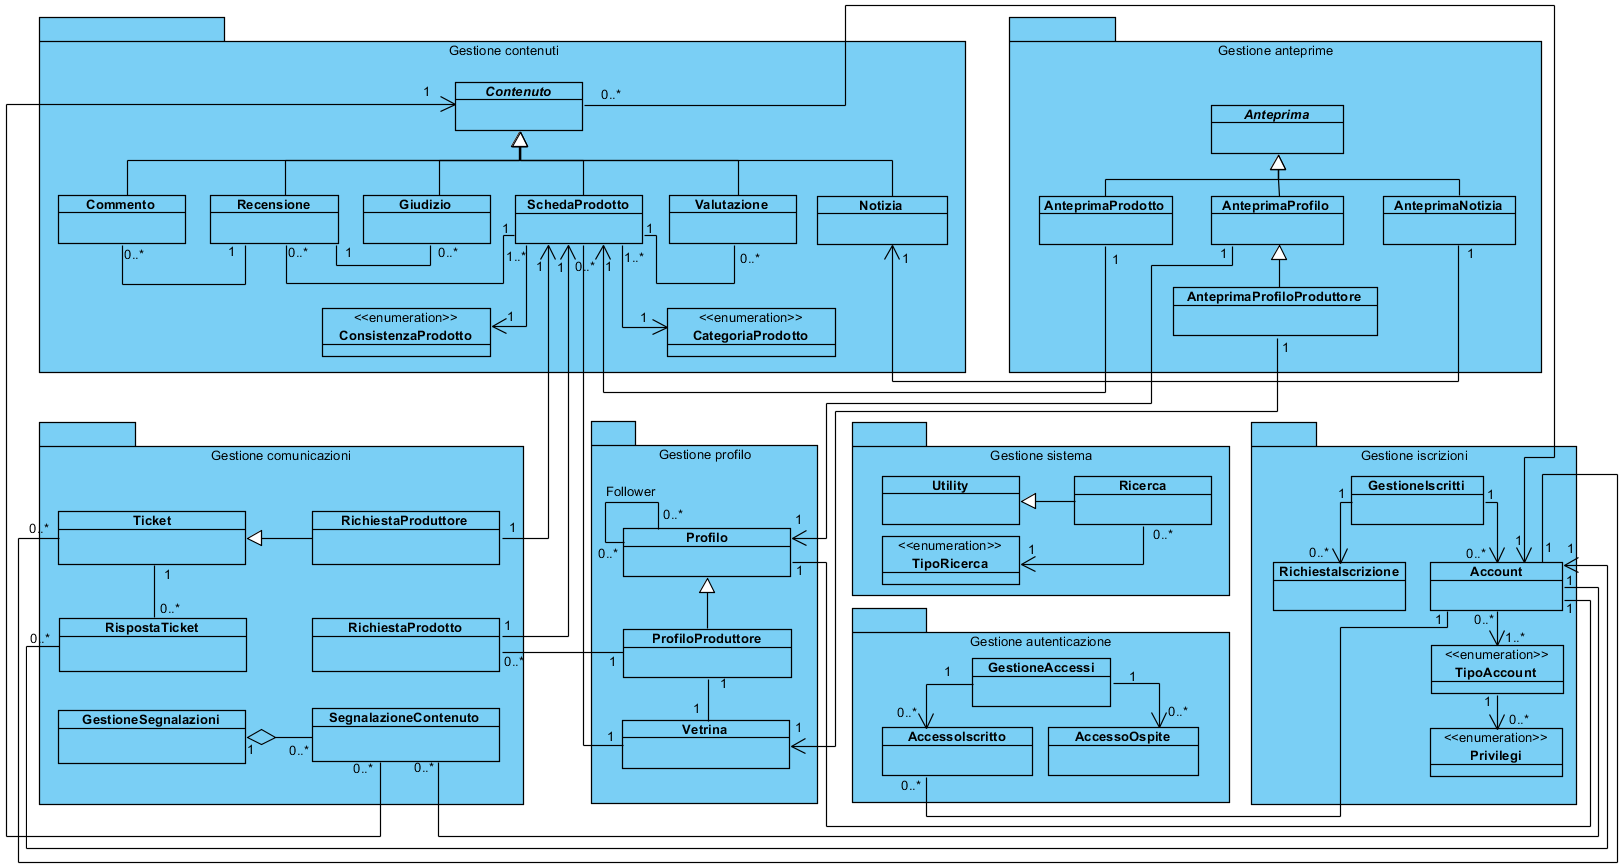
\includegraphics[width=\linewidth]{assets/visualParadigm/package/DiagrammaPacakage}
\end{center}
\end{landscape}

\section{Diagrammi delle classi}
I diagrammi delle classi servono a modellare la relazione tra le entità del sistema, rappresentate come classi.
Una classe è composta da delle caratteristiche che la descrivono (attributi) e delle elaborazioni che vengono eseguite (metodi). 
Le classi servono ad identificare chi fa che cosa e come all’interno del sistema. Queste possono avere relazioni tra loro, le quali sono rappresentate con le associazioni. La cardinalità di un’associazione esprime il numero di oggetti di una certa classe che prendono parte all’associazione.
È inoltre possibile associare una nota ad una classe per descrivere il modello che la classe definisce.
Di seguito sono elencati i diagrammi di sequenza, non verranno riportati tutti i diagrammi di sequenza, ma solo quelli corrispondenti ai casi d'uso principali.
\begin{itemize}
	\item \newPKG{pkg:GestioneAnteprime}{\formattaPKG}{Gestione anteprima}
	\item \newPKG{pkg:GestioneAutenticazione}{\formattaPKG}{Gestione autenticazione}
	\item \newPKG{pkg:GestioneIscritti}{\formattaPKG}{Gestione iscritti}
	\item \newPKG{pkg:GestioneTicket}{\formattaPKG}{Gestione ticket}
	\item \newPKG{pkg:GestioneProfilo}{\formattaPKG}{Gestione profilo}
	\item \newPKG{pkg:GestioneContenuti}{\formattaPKG}{Gestione contenuti}
	\item \newPKG{pkg:GestioneSistema}{\formattaPKG}{Gestione sistema}
\end{itemize}

\linkedSubsection{pkg:GestioneAnteprime}
\begin{center}
			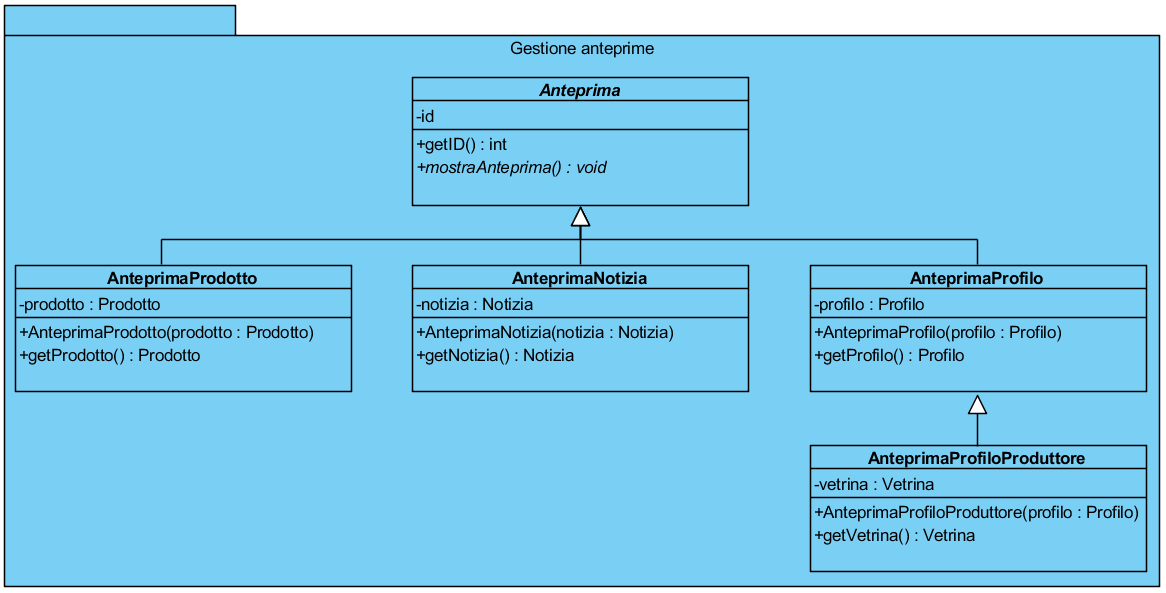
\includegraphics[width=\textwidth]{assets/visualParadigm/classi/GestioneAnteprime}
\end{center}

\linkedSubsection{pkg:GestioneAutenticazione}
\begin{center}
			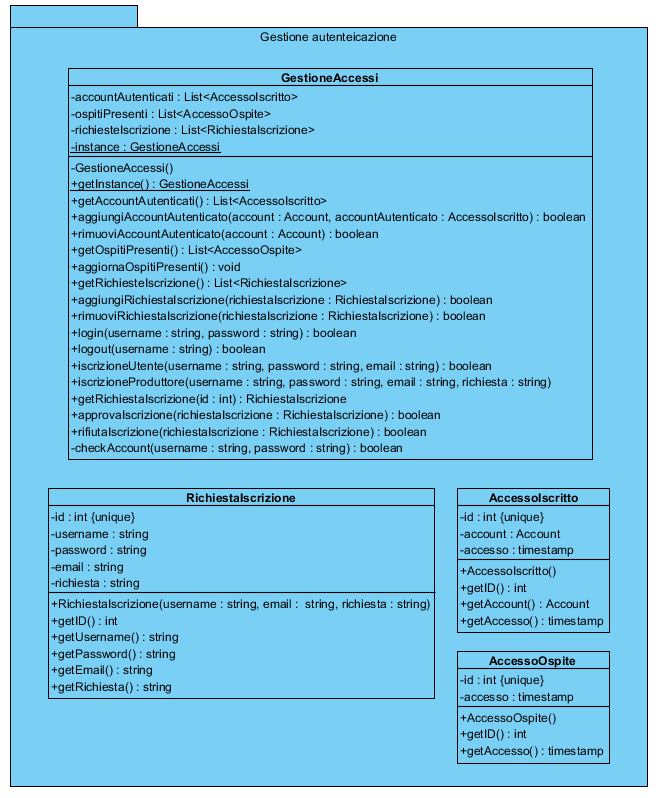
\includegraphics[width=\textwidth]{assets/visualParadigm/classi/GestioneAutenticazione}
\end{center}

\linkedSubsection{pkg:GestioneIscritti}
\begin{center}
			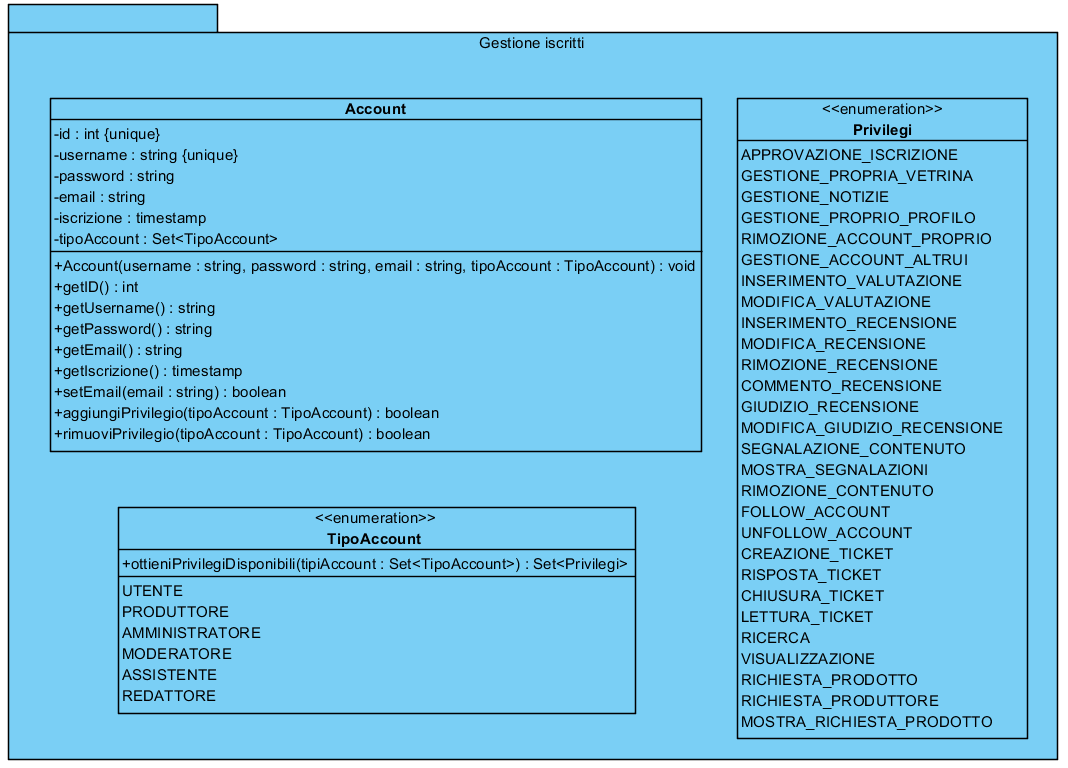
\includegraphics[width=\textwidth]{assets/visualParadigm/classi/GestioneIscritti}
\end{center}

\linkedSubsection{pkg:GestioneTicket}
\begin{center}
			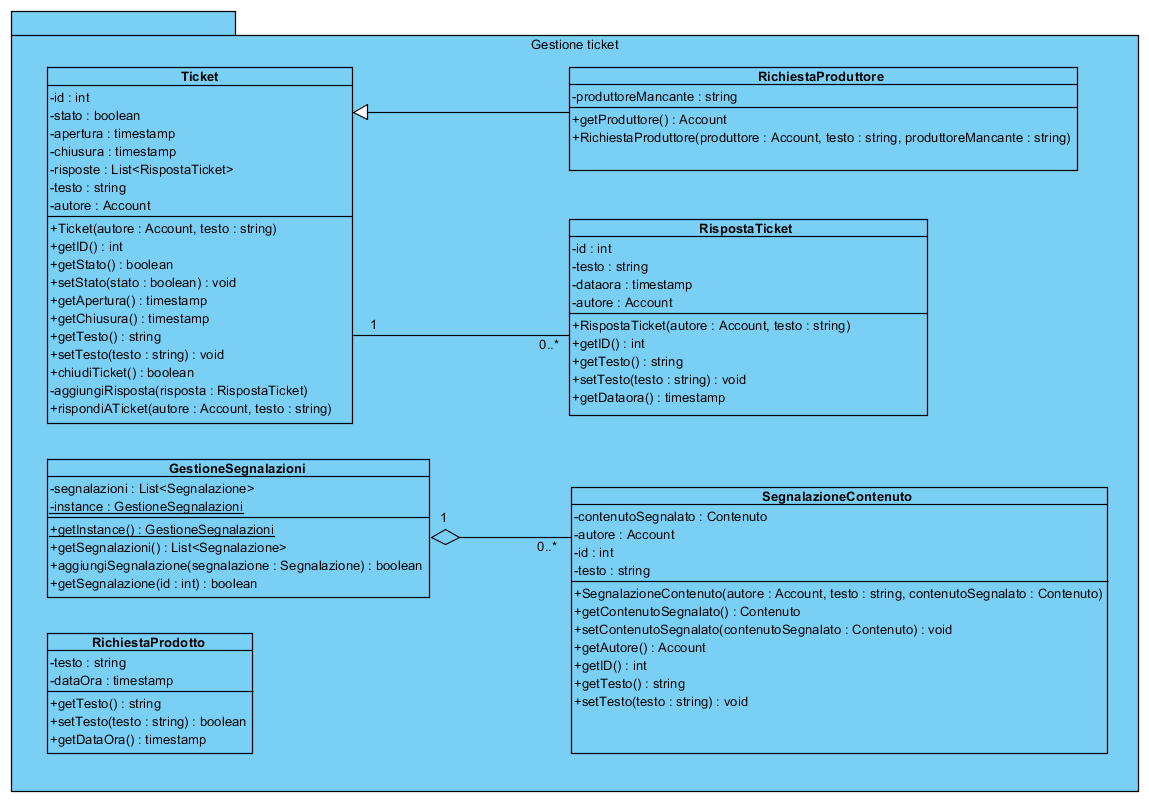
\includegraphics[width=\textwidth]{assets/visualParadigm/classi/GestioneTicket}
\end{center}

\begin{landscape}
\linkedSubsection{pkg:GestioneProfilo}
\begin{center}
			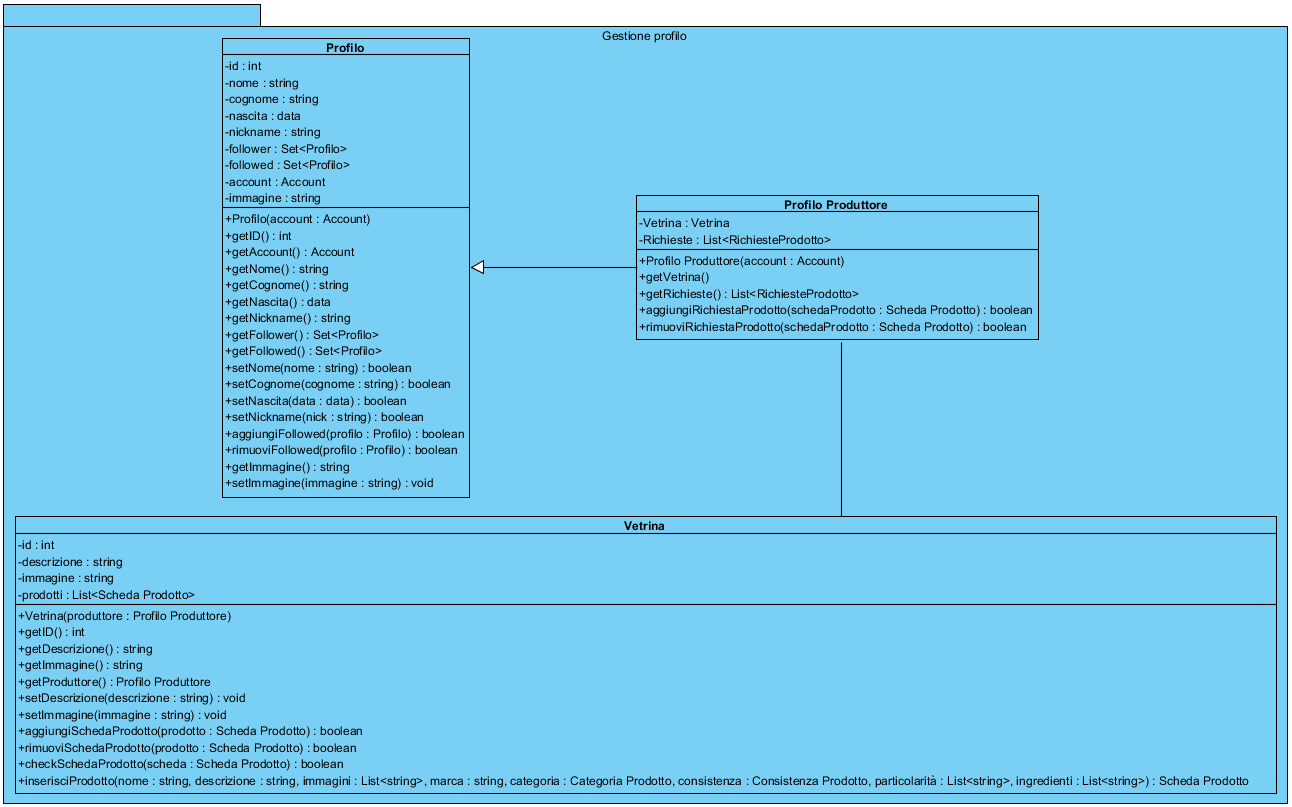
\includegraphics[width=1.1\linewidth]{assets/visualParadigm/classi/GestioneProfilo}
\end{center}
\end{landscape}

\begin{landscape}
\linkedSubsection{pkg:GestioneContenuti}
\begin{center}
			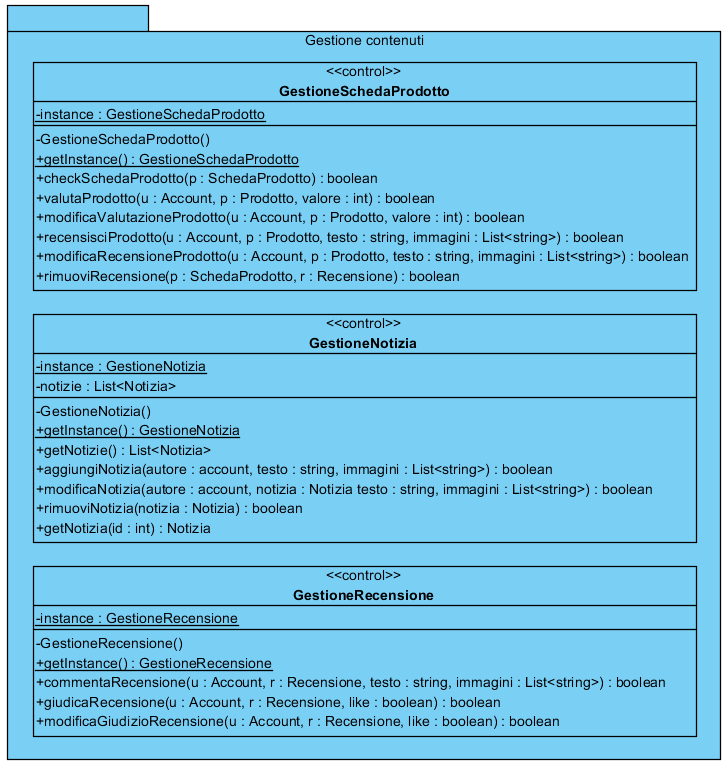
\includegraphics[width=1.1\linewidth]{assets/visualParadigm/classi/GestioneContenuti}
\end{center}
\end{landscape}

\linkedSubsection{pkg:GestioneSistema}
\begin{center}
			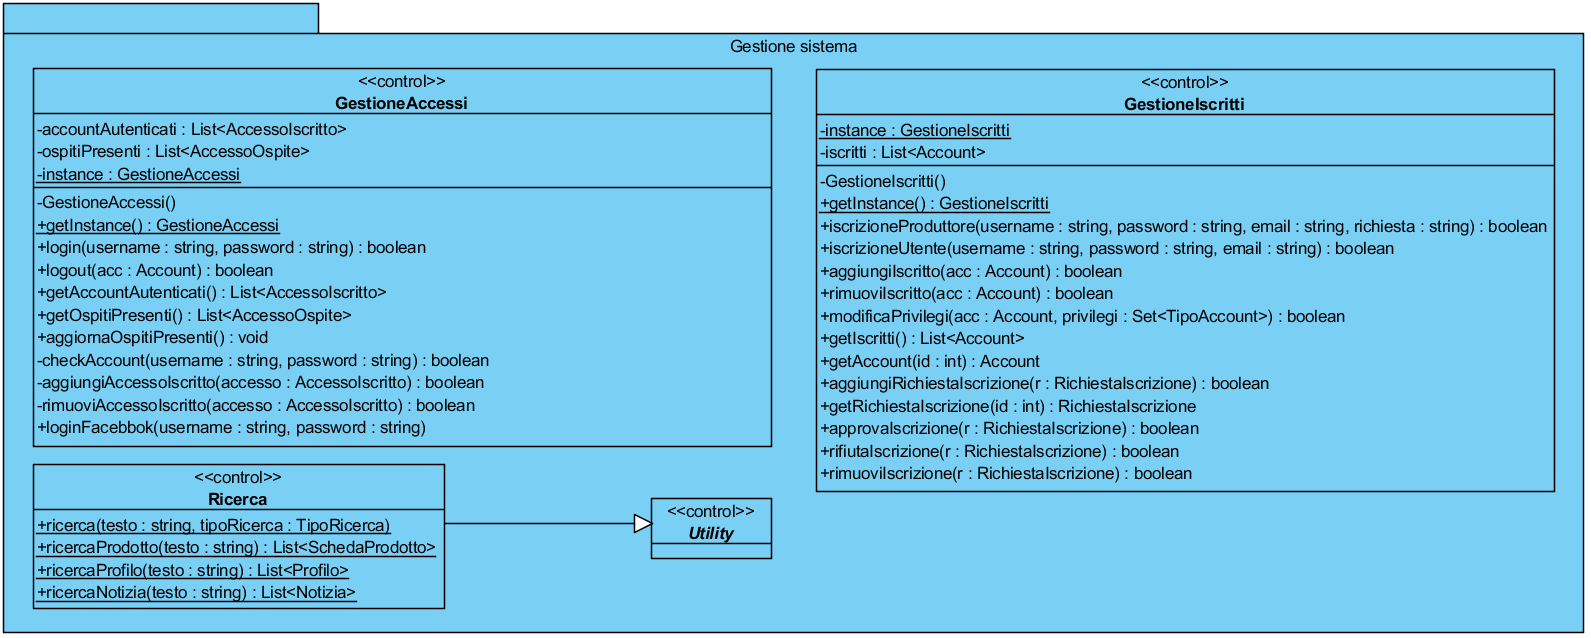
\includegraphics[width=\textwidth]{assets/visualParadigm/classi/GestioneSistema}
\end{center}


\section{Diagrammi di sequenza}
I diagrammi di sequenza descrivono le interazioni tra gli oggetti organizzate in sequenza temporale. Ogni caso d’uso contiene al suo interno diversi diagrammi di sequenza. Rappresenteremo solo le sequenze principali.
Un diagramma di sequenza è costituito da:
\begin{itemize}
	\item Gli oggetti
	\item I messaggi attraverso cui essi interagiscono
\end{itemize}
Di seguito sono elencati i diagrammi di sequenza, non verranno riportati tutti i diagrammi di sequenza, ma solo quelli corrispondenti ai casi d'uso principali.
\begin{itemize}
	\item \newSequenza{seq:login}{\formattaSEQ}{Login}
	\item \newSequenza{seq:logout}{\formattaSEQ}{Logout}
	\item \newSequenza{seq:iscrizioneProduttore}{\formattaSEQ}{Iscrizione Produttore}
	\item \newSequenza{seq:iscrizioneUtente}{\formattaSEQ}{Iscrizione Utente}
	\item \newSequenza{seq:approvazioneIscrizione}{\formattaSEQ}{Approvazione iscrizione}
	\item \newSequenza{seq:inserimentoSchedaProdotto}{\formattaSEQ}{Inserimento scheda prodotto}
	\item \newSequenza{seq:inserimentoValutazione}{\formattaSEQ}{Inserimento valutazione}
	\item \newSequenza{seq:inserimentoRecensione}{\formattaSEQ}{Inserimento recensione}
	\item \newSequenza{seq:rimuoviRecensione}{\formattaSEQ}{Rimuovi recensione}
	\item \newSequenza{seq:commentoRecensione}{\formattaSEQ}{Commento recensione}
	\item \newSequenza{seq:giudicaRecensione}{\formattaSEQ}{Giudica recensione}
	\item \newSequenza{seq:ricerca}{\formattaSEQ}{Ricerca}
\end{itemize}

\linkedSubsection{seq:login}
\begin{center}
			\includegraphics[width=\textwidth]{assets/visualParadigm/sequenza/login}
\end{center}

\linkedSubsection{seq:logout}
\begin{center}
			\includegraphics[width=\textwidth]{assets/visualParadigm/sequenza/logout}
\end{center}

\linkedSubsection{seq:iscrizioneProduttore}
\begin{center}
			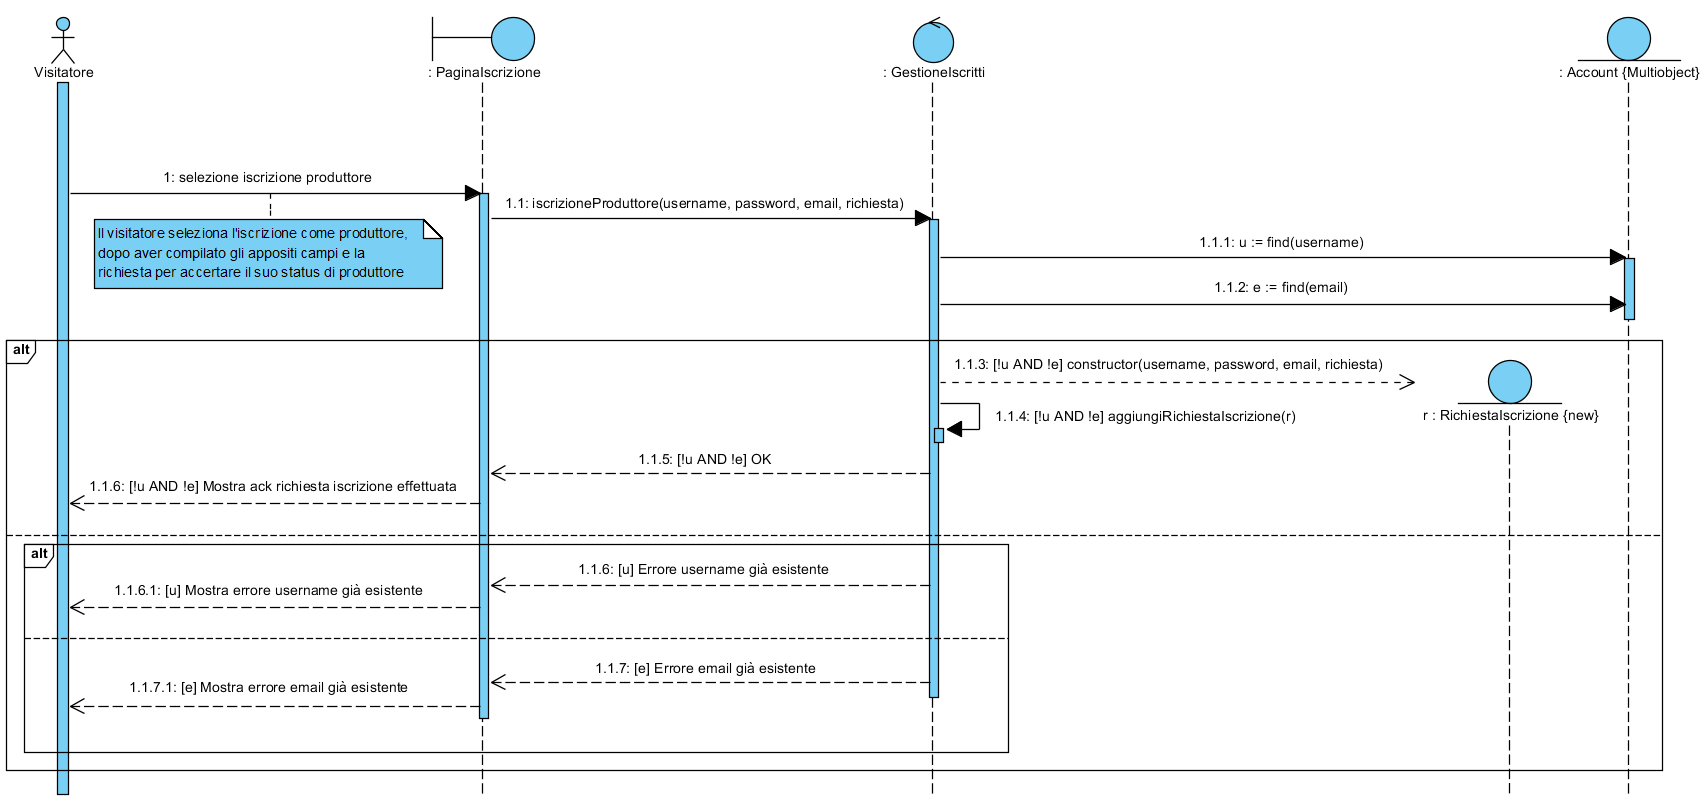
\includegraphics[width=\textwidth]{assets/visualParadigm/sequenza/iscrizioneProduttore}
\end{center}

\linkedSubsection{seq:iscrizioneUtente}
\begin{center}
			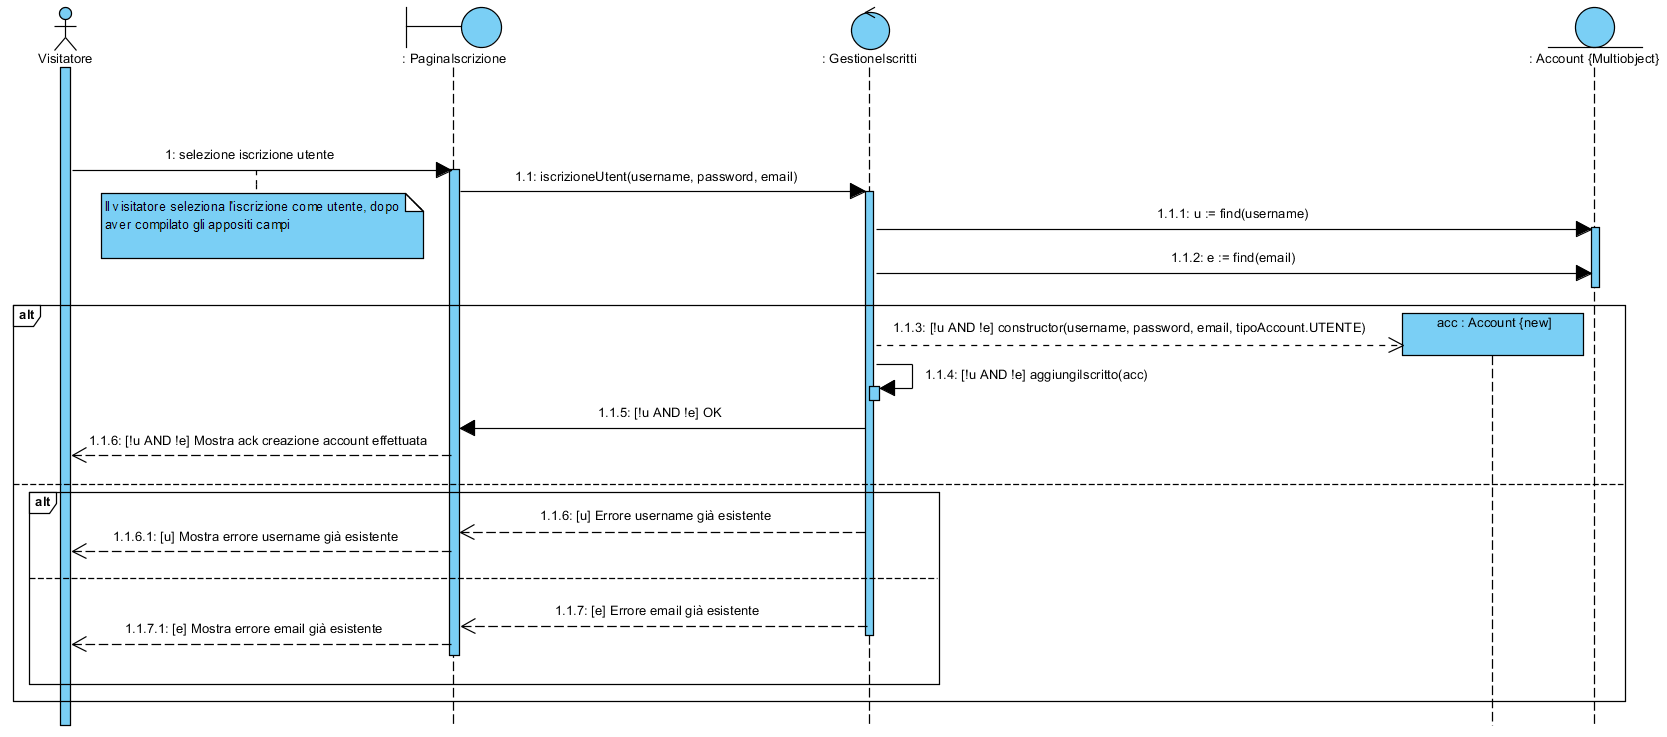
\includegraphics[width=\textwidth]{assets/visualParadigm/sequenza/iscrizioneUtente}
\end{center}

\linkedSubsection{seq:approvazioneIscrizione}
\begin{center}
			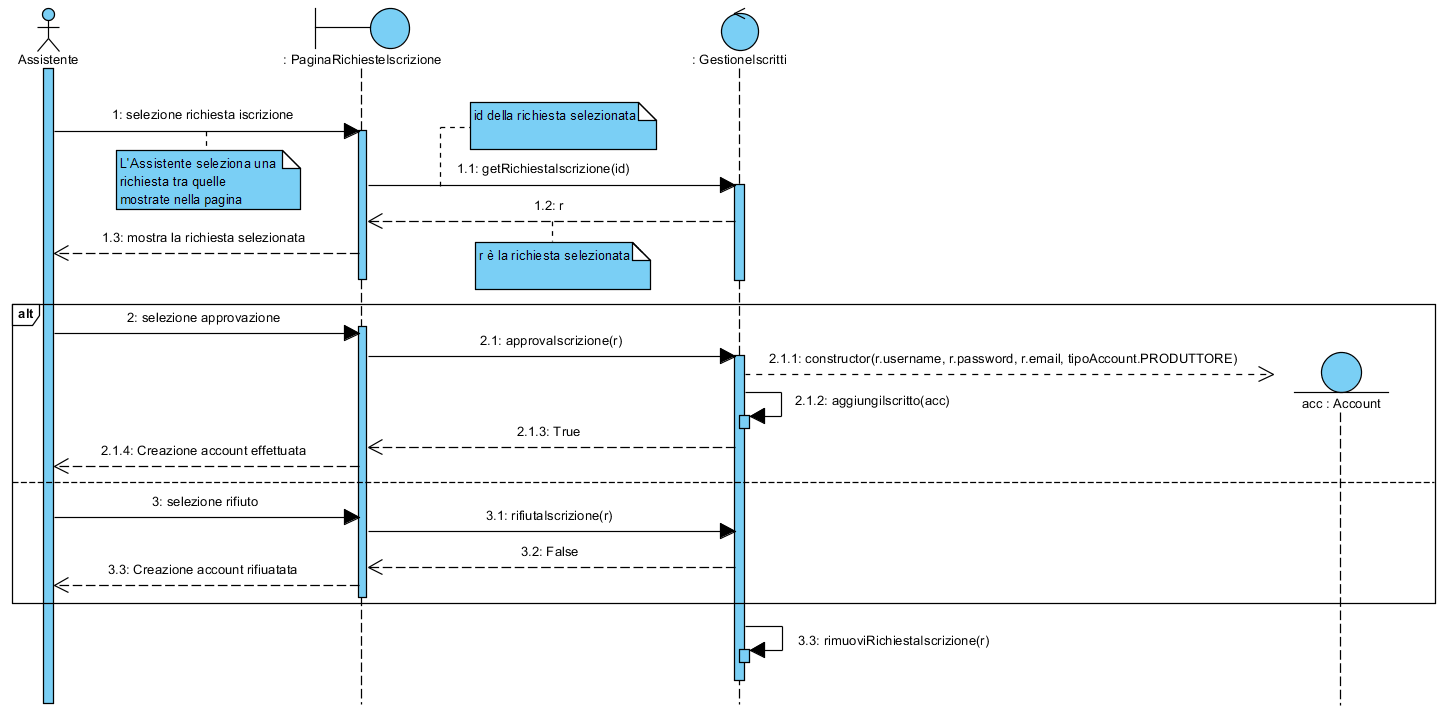
\includegraphics[width=\textwidth]{assets/visualParadigm/sequenza/approvazioneIscrizione}
\end{center}

\linkedSubsection{seq:inserimentoSchedaProdotto}
\begin{center}
			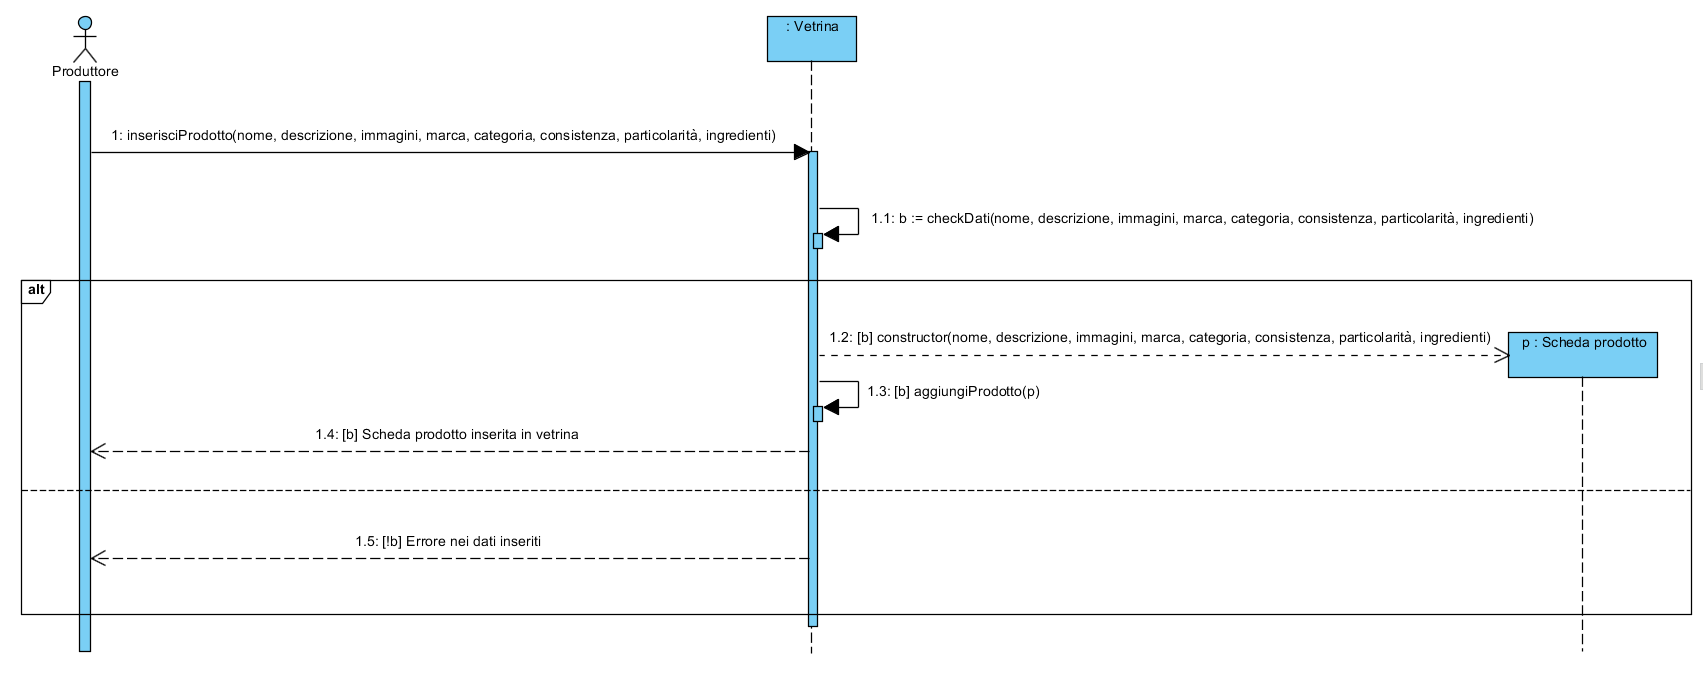
\includegraphics[width=\textwidth]{assets/visualParadigm/sequenza/inserimentoSchedaProdotto}
\end{center}

\linkedSubsection{seq:inserimentoValutazione}
\begin{center}
			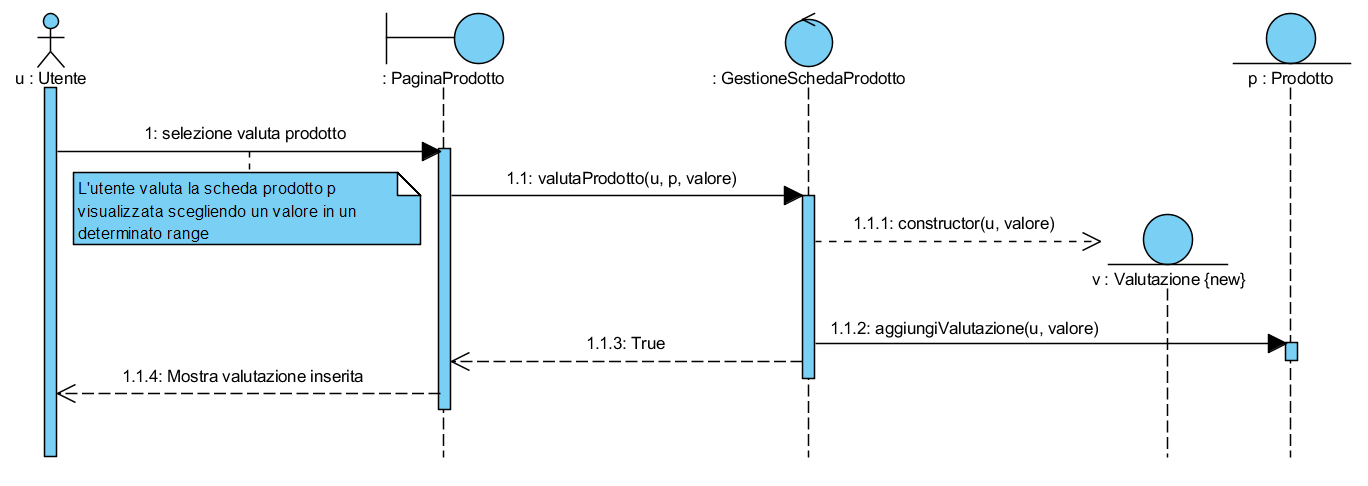
\includegraphics[width=\textwidth]{assets/visualParadigm/sequenza/inserimentoValutazione}
\end{center}

\linkedSubsection{seq:inserimentoRecensione}
\begin{center}
			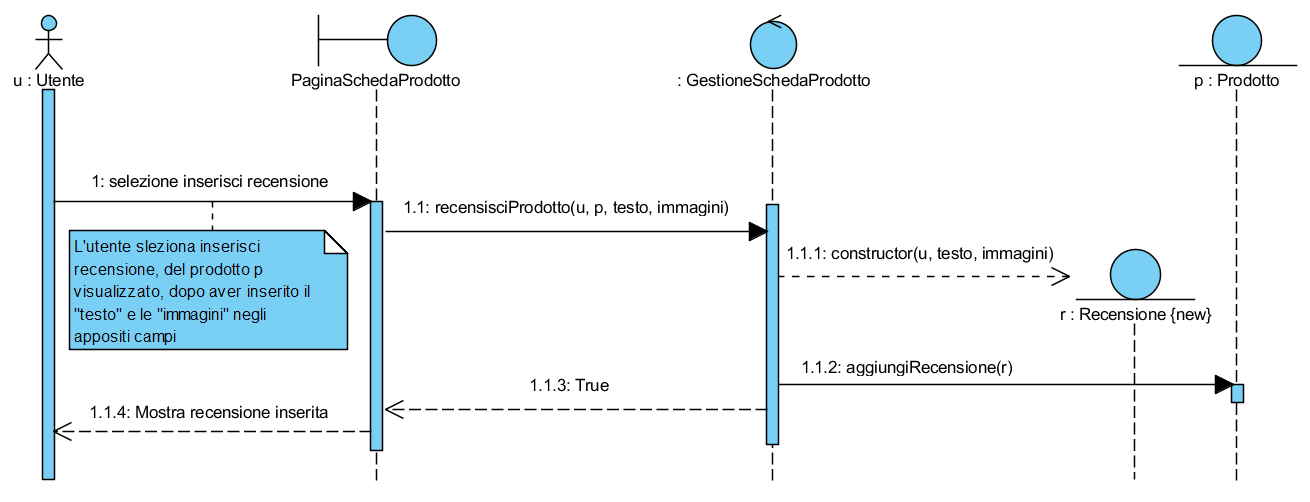
\includegraphics[width=\textwidth]{assets/visualParadigm/sequenza/inserimentoRecensione}
\end{center}

\linkedSubsection{seq:rimuoviRecensione}
\begin{center}
			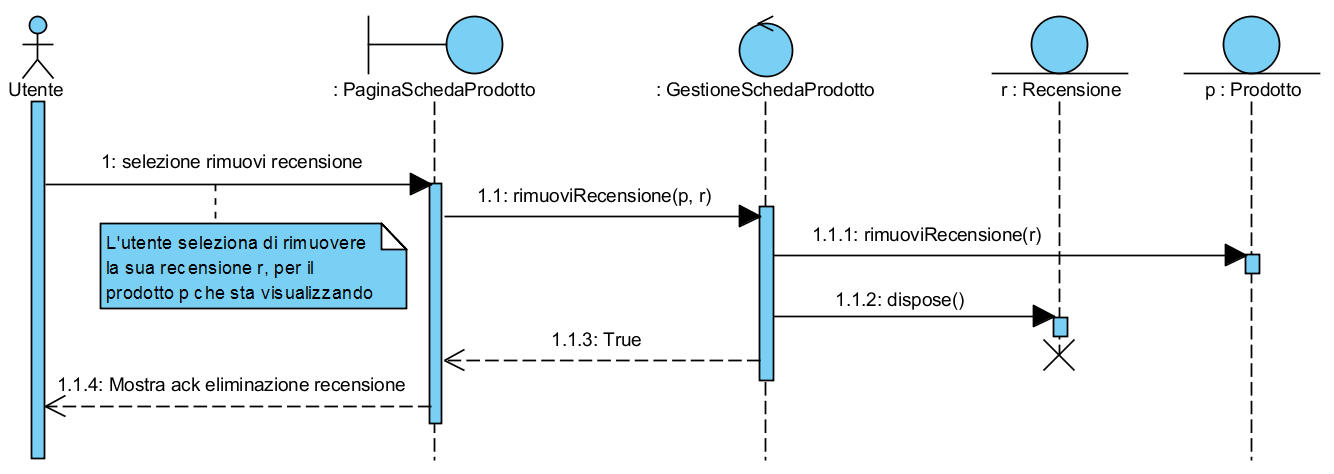
\includegraphics[width=\textwidth]{assets/visualParadigm/sequenza/rimuoviRecensione}
\end{center}

\linkedSubsection{seq:commentoRecensione}
\begin{center}
			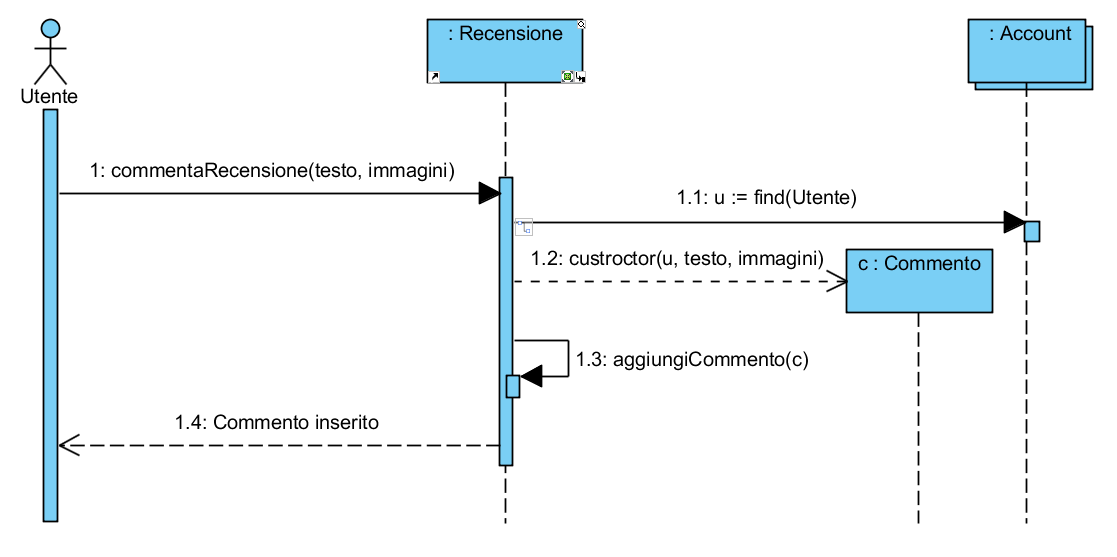
\includegraphics[width=\textwidth]{assets/visualParadigm/sequenza/commentoRecensione}
\end{center}

\linkedSubsection{seq:giudicaRecensione}
\begin{center}
			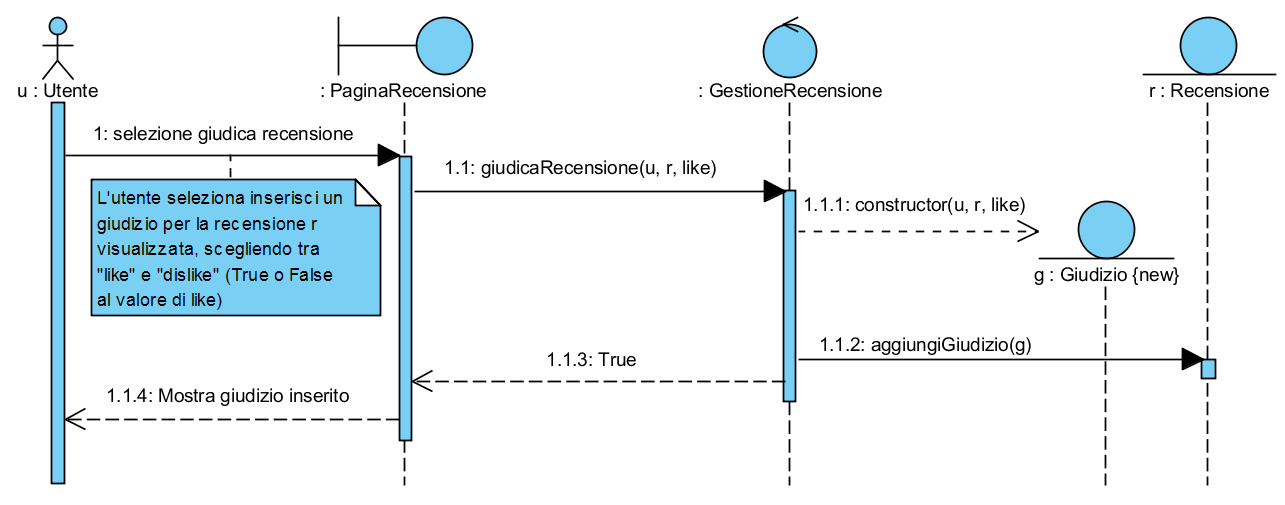
\includegraphics[width=\textwidth]{assets/visualParadigm/sequenza/giudicaRecensione}
\end{center}

\linkedSubsection{seq:ricerca}
\begin{center}
			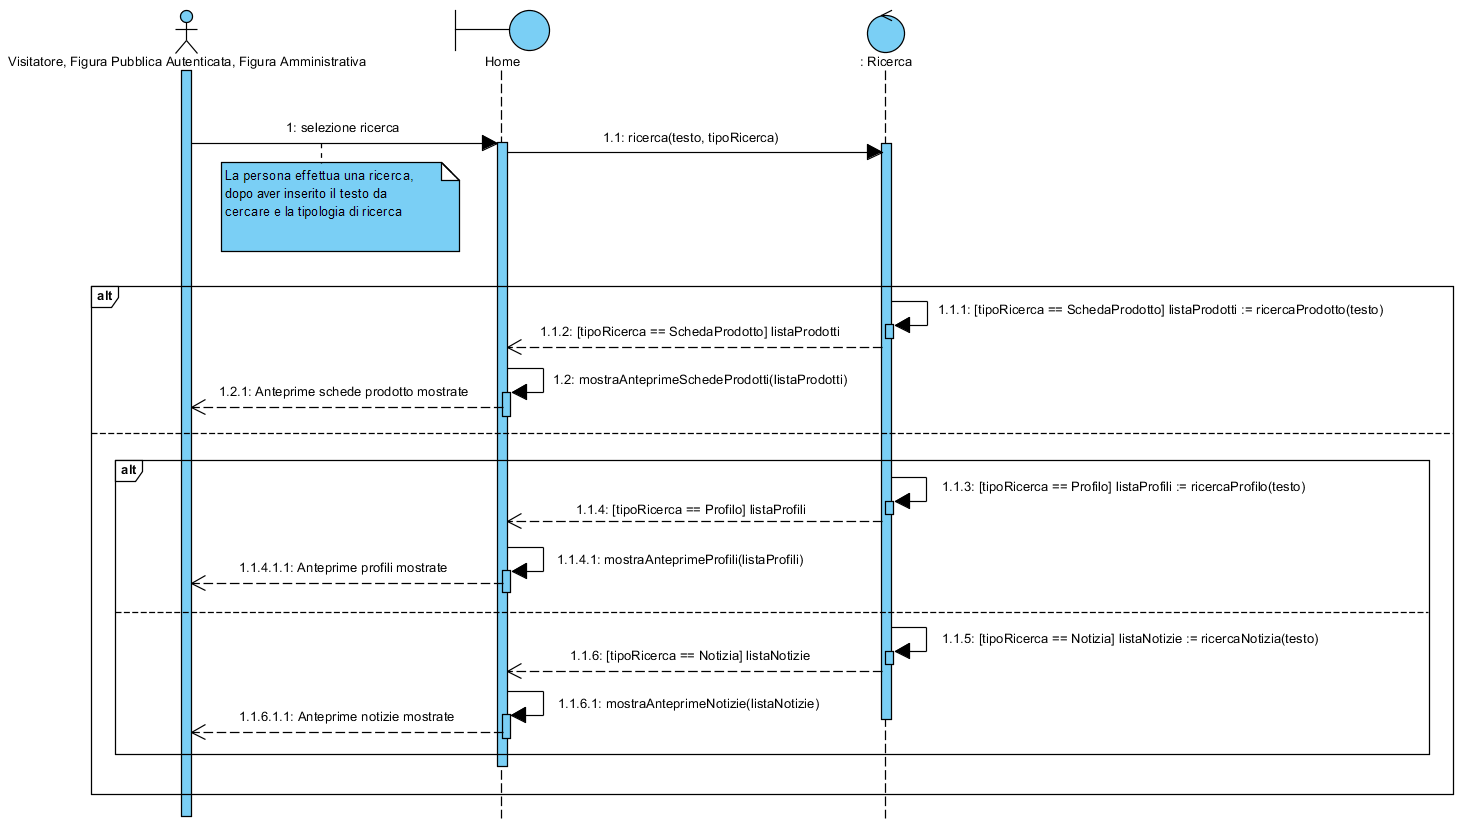
\includegraphics[width=\textwidth]{assets/visualParadigm/sequenza/ricerca}
\end{center}


\begin{comment}
-	CU.A.1 - Login
-	CU.A.3 - Logout
-	CU.B.1 - Iscrizione tramite modulo
-	CU.B.2 - Iscrizione tramite Social Network
-	CU.B.3 - Iscrizione tramite approvazione
-	CU.B.4 - Approvazione iscrizione
-	CU.C.5 - Inserimento scheda prodotto

	CU.G.1 - Inserimento valutazione
	CU.H.1 - Inserimento recensione
	CU.H.4 - Commento a recensione
	CU.H.5 - Giudizio recensione

-	CU.K.1 - Ricerca prodotto
-	CU.K.2 - Ricerca profilo
-	CU.K.3 - Ricerca notizia
-	CU.M.1 - Mostra vetrina
-	CU.M.2 - Mostra scheda prodotto
-	CU.M.4 - Mostra recensione
-	CU.M.5 - Mostra profilo pubblico
-	CU.M.6 - Mostra notizia
\end{comment}

    \chapter{Design del sistema}

\section{Introduzione}
In questo documento mostreremo delle soluzioni concrete per il modello di analisi effettuato nel documento di \docref{cha:analisi}, aggiungeremo quindi il \emph{come} al \emph{cosa}. Mostreremo quindi una specifica architetture del sistema e aggiungeremo il necessario per rendere possibile l'implementazione dei requisiti formalizzati nel documento di \docref{cha:specifica_requisiti}.

\section{Architettura del sistema}
Vengono di seguito mostrate l'architettura fisica e quella software del sistema.

\subsection{Architettura fisica}
L'architettura fisica del sistema è mostrata dalla seguente figura:
\begin{center}
   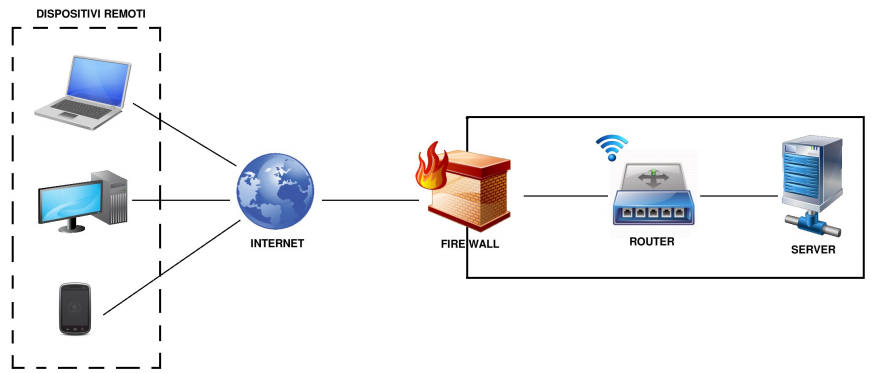
\includegraphics[width=\textwidth]{assets/architetturaFisica}
\end{center}

\subsection{Architettura software}
L'architettura software del sistema è mostrata dalla seguente figura:
\begin{center}
   \includegraphics[width=\textwidth]{assets/architetturaSoftware}
\end{center}

\section{CMS}
Per realizzare il sistema finora descritto utilizzeremo il \gls{cms} commerciale WordPress, scelto in quanto dispone di una grande quantità di plugin per soddisfare tutte le funzionalità precedentemente descritte. Questo sarà installato nel server e si occuperà della comunicazione con i fruitori del servizio e integrerà il database.

\subsection{Installazione}
Per installare WordPress sarà necessario seguire i seguenti passi:
\begin{enumerate}
	\item Scaricare e decomprimere il pacchetto di WordPress;
	\item Creare un database per WordPress sul server web, ed un utente MySQL che abbia tutti i permessi per accederci e modificarlo;
	\item Rinominare il file \texttt{wp-config-sample.php} in \texttt{wp-config.php};
	\item Aprire \texttt{wp-config.php} in un editor di testo e inserire i dettagli del database;
	\item Caricare i file di WordPress nella cartella principale del server web;
	\item Lanciare lo script di installazione di WordPress visitando la pagina \texttt{http://esempio.com/wp-admin/install.php};
\end{enumerate}

\subsection{Configurazione}
Si dovranno creare le pagine descritte in fase di analisi, abilitare l'iscrizione ed il login al sito.

\subsection{Plugin}
WordPress mette a disposizione oltre 47mila plugin, i quali estendono ed espandono le funzionalità di base presenti.
L'installazione e l'attivazione dei plugin è immediata, in quanto è possibile effettuarla direttamente tramite il pannello di controllo di WordPress.
Per implementare tutte le funzionalità precedentemente descritte sarà necessario installare ed attivare i seguenti plugin.

\subsubsection{User Role Editor}
\paragraph{Descrizione.} Con il plugin \gls{ure} è possibile cambiare le capacità del ruolo utente semplicemente. Basta spuntare le caselle di controllo delle capacità che si desidera aggiungere al ruolo selezionato. Aggiungere nuovi ruoli e personalizzarne le capacità in base alle proprie esigenze. Il ruolo creato automaticamente può essere eliminato se non ci sono utenti a cui tale ruolo è assegnato. Anche il ruolo assegnato di default alla creazione di ogni nuovo utente può essere modificato. Le capacità possono essere assegnate sulla base del singolo utente. Ruoli multipli possono essere assegnati all'utente simultaneamente. È possibile aggiungere nuove funzionalità e rimuovere le funzionalità non necessarie che potrebbero essere state lasciate da un plugin disinstallato.
\paragraph{Utilizzo.} \gls{ure} potrà essere utilizzato dall'amministratore per la gestione dei ruoli, dei profili, degli account e dell'assegnamento dei privilegi in base a quali ruoli un account possiede.
\paragraph{Configurazione.} Si dovranno creare i ruoli Visitatore, Utente, Produttore, Assistente, Redattore, Moderatore e Amministratore, assegnando ad ognuno i corrispettivi privilegi.

\subsubsection{Multiple Registration Forms}
\paragraph{Descrizione.} Il plugin \gls{mrf} permette di creare form di iscrizione multipli, in base a quale tipologia di account si vuole creare
\paragraph{Utilizzo.}  \gls{mrf} potrà essere utilizzato per creare i form di registrazione per utenti e produttori.
\paragraph{Configurazione.}  Si dovranno creare i form di registrazione per gli utenti e i produttori.

\subsubsection{Profile Builder Pro}
\paragraph{Descrizione.} Il plugin \gls{pbp} permette di creare profili altamente personalizzabili, è possibile inoltre personalizzare il form di iscrizione, login e recupero password. 
\paragraph{Utilizzo.}  \gls{pbp} potrà essere utilizzato per creare i profili utente e produttore, e approvare le richieste di iscrizione produttore.
\paragraph{Configurazione.}  Si dovranno creare i profili descritti e associarli agli account in base al loro ruolo. Si dovrà impostare l'iscrizione previa approvazione per le registrazioni di produttori

\subsubsection{WP User Frontend}
\paragraph{Descrizione.} Questo plugin fornisce alle persone autenticate la possibilità di creare nuovi post, di modificare i propri profili direttamente dal fronted, senza dover accedere al pannello di amministrazione.
\paragraph{Utilizzo.}  \gls{wpuf} potrà essere utilizzato dall'amministratore per fornire alle persone autenticate la possibilità di modificare i propri profili direttamente dal fronted.
\paragraph{Configurazione.} Si dovrà dare alle persone iscritte la possibilità di personalizzare il profilo in base al ruolo posseduto.

\subsubsection{WooCommerce}
\paragraph{Descrizione.} \gls{wc} è un plugin per e-commerce gratuito che ti permette di vendere in maniera ottimale qualsiasi cosa. \gls{wc}fornisce sia ai proprietari che agli sviluppatori il controllo completo del proprio shop.
\paragraph{Utilizzo.} \gls{wc} potrà essere utilizzato per gestire la vetrina e l'inserimento e la modifica di prodotti, recensioni ad essi associate, commenti a recensioni, valutazioni e giudizi.
\paragraph{Configurazione.} Si dovrà configurare \gls{wc} in modo da non permettere la vendita di prodotti, ma solo la loro esposizione.
Per permettere a più produttori di avere la propria vetrina sarà necessaria l'installazione di \gls{wcv}.

\subsubsection{WC Vendors}
\paragraph{Descrizione.} Questo plugin permette di creare il proprio marketplace e di fornire ai venditori la possibilità di vendere come su etsy, Envato, eBay, o Amazon. \gls{wcv} permette a più venditori di vendere i propri prodotti.
\paragraph{Utilizzo.} \gls{wcv} potrà essere utilizzato per gestire più vetrine contemporaneamente, permettendo ad ogni produttore di avere la propria vetrina in cui mostrare i propri prodotti.
\paragraph{Configurazione.} Non necessita di configurazione particolare.

\subsubsection{BuddyPress}
\paragraph{Descrizione.}
BuddyPress è una insieme di componenti comuni a un tipico social network, e permette di aggiungere molte funzionalità attraverso l'esteso sistema di plugin di WordPress.
BuddyPress è focalizzato sulla facilità di integrazione, facilità d'uso e estensibilità. È un software per creare social network volutamente potente anche se incredibilmente semplice, costruito dai contributori di WordPress.
Consenti ai membri di registrarsi per aprire un profilo, avere conversazioni private, effettuare collegamenti, creare per interagire nei gruppi, e molto altro. 
\paragraph{Utilizzo.}
\gls{bp} potrà essere utilizzato per gestire il lato social del sistema, oltre a gestire le richieste dagli utenti ai produttori.
\paragraph{Configurazione.}
Per configurare BuddyPress e gestire il sistema di follower/followed è necessario installare il plugin \gls{bpf}

\subsubsection{BuddyPress Follow}
\paragraph{Descrizione.}
Questo plugin permette di estendere le funzionalità di \gls{bp} per implementare il sistema di follower/followed .
\paragraph{Utilizzo.} Verrà utilizzato per implementare il sistema di follower/followed.
\paragraph{Configurazione.} Non necessita di configurazione particolare.

\subsubsection{WP Support Plus Responsive Ticket System}
\paragraph{Descrizione.} Questo plugin aggiunge a WordPress le funzionalità di un sistema di ticket completo. Permette alle persone autenticate di creare ticket per segnalare problemi o per ottenere supporto. I creatori del ticket possono impostare lo stato, la priorità e la categoria del ticket.
\paragraph{Utilizzo.} Questo plugin potrà essere utilizzato dalle persone autenticate per creare ticket per ottenere supporto.
\paragraph{Configurazione.} Non necessita di configurazione particolare.

\subsubsection{WP Report Post}
\paragraph{Descrizione.} Questo plugin permette di segnalare post o pagine con contenuti inappropriati. Tutti questi report sono mostrati in una tabella nella sezione di Amministratore, permettendo così a quest'ultimo di scegliere cosa fare: modificare i contenuti, cancellare la pubblicazione di post/pagine, o semplicemente di eliminare i report. \gls{wprp} è progettato per funzionare sia in modo automatico che in modo manuale. In modo automatico, il link per segnalare potrà essere aggiunto al meta box del post. In modo manuale, si può aggiungere il link, il bottone o l'immagine dove si vuole nel template.
\paragraph{Utilizzo.} \gls{wprp} potrà essere utilizzato per inserire la possibilità di segnalare i contenuti del sistema, come schede prodotto, recensioni o commenti.
\paragraph{Configurazione.} Si dovrà configurare il link/bottone/immagine per effettuare la segnalazione su ogni contenuto segnalabile.

\subsubsection{Ninja Forms}
\paragraph{Descrizione.} Questo plugin permette la creazione di form utilizzando un seplice drag-and-drop. Per i principianti è presente un design di creazione form semplice senza la necessità di scrivere codice. Gli sviluppatori, invece, possono utilizzare opzioni built-in, filtri, e template di campi personalizzati per la creazione di form di ogni tipo e anche per la loro sottomissione.
\paragraph{Utilizzo.} \gls{nf} potrà essere utilizzato per permettere la creazione dei form necessari all'interno del sistema.
\paragraph{Configurazione.} Non necessita di configurazione particolare.

\subsubsection{Nextend Facebook Connect}
\paragraph{Descrizione.} Questo plugin permette la registrazione ed il login tramite Facebook.
\paragraph{Utilizzo.} \gls{nfc} potrà essere utilizzato per permettere agli Visitatori di creare un account di tipo Utente utilizzando la registrazione tramite Facebook. Sarà perciò possibile effettuare il login con le credenziali di Facebook.
\paragraph{Configurazione.} Si dovranno configurare il bottone per effettuare la registrazione e quello per effettuare il login tramite Facebook.

\newdate{designuno}{24}{10}{2016}
\section{Revisioni}
\begin{center}
	\begin{tabular}{lll}
		\toprule
		\tabhead{Versione} & \tabhead{Data} & \tabhead{Descrizione} \\
		\cmidrule(l{\cmidrulekern}r{\cmidrulekern}){1-3}
		1.0 & \displaydate{designuno} & Prima versione \\        
		\bottomrule
	\end{tabular}
\end{center}

    \chapter{Documento dei piani di test}
\section{Introduzione}
In questo documento vengono definiti i test funzionali, necessari per garantire il corretto comportamento del sistema.
L'utilizzo di un \gls{cms} commerciale e dei suoi plugin, di cui assumiamo corretto il funzionamento (in quanto prodotti ampiamente diffusi e utilizzati negli ambiti più disparati con successo), ci permette di ridurre il numero di test necessari.
Infatti i \docref{sub:requisiti_non_funzionali} possono essere considerati come soddisfatti, così come alcuni dei \docref{sub:requisiti_funzionali}.

\section{Elenco test funzionali}
I test funzionali garantiscono il rispetto dei casi d'uso da parte del sistema.
Vengono di seguito elencati i test funzionali:
\begin{itemize}
	\item \newTestItem{cu:login}
	\item \newTestItem{cu:logout}
	\item \newTestItem{cu:iscrizionePortale}
	\item \newTestItem{cu:iscrizioneApprovazione}
	\item \newTestItem{cu:approvazioneIscrizione}
	\item \newTestItem{cu:personalizzaVetrinaInsProd}
	\item \newTestItem{cu:inserisciRecensioneProdotto}
	\item \newTestItem{cu:eliminaRecensioneProdotto}
	\item \newTestItem{cu:commentoRecensione}
	\item \newTestItem{cu:giudizioRecensione}
	\item \newTestItem{cu:ricercaProdotto}
	\item \newTestItem{cu:ricercaProfilo}
	\item \newTestItem{cu:ricercaNotizia}
\end{itemize}

\section{Descrizione test funzionali}
%{Obiettivo}{Prerequisiti}{Azioni}
\testTab{cu:login}
{Testare il corretto funzionamento della funzionalità di Login, controllando anche che in caso di inserimento di dati errati venga restituito l'errore previsto}
{Le credenziali corrette sono presenti nel sistema, le credenziali errate non sono presenti nel sistema. La persona non è autenticata nel sistema}
{\begin{enumerate}
	\item Inserire le credenziali corrette
	\item Effettuare il Login
	\item Verificare che il Login abbia successo
	\item Effettuare il Logout
	\item Inserire le credenziali errate
	\item Verificare che il Login non abbia successo e che venga mostrato l'errore previsto
\end{enumerate}
}

\vspaceTab

\testTab{cu:logout}
{Testare il corretto funzionamento della funzionalità di Logout}
{La persona è autenticata nel sistema}
{\begin{enumerate}
	\item Effettuare il Logout
	\item Verificare che la persona venga disconnessa dal sistema
\end{enumerate}
}

\vspaceTab

\testTab{cu:iscrizionePortale}
{Testare il corretto funzionamento della funzionalità di registrazione al sistema per creare account di tipo Utente}
{Le credenziali corrette non sono presenti nel sistema, le credenziali errate sono già usate da un altro account. La persona non è utenticata nel sistema}
{\begin{enumerate}
	\item Avviare la procedura di registrazione per creare un account Utente
	\item Compilare il form con le credenziali corrette
	\item Confermare l'operazione di registrazione e verificare che avvenga con successo
	\item Avviare la procedura di registrazione per creare un account Utente
	\item Compilare il form con le credenziali errate
	\item Confermare l'operazione di registrazione e verificare che venga mostrato l'errore previsto
\end{enumerate}}

\vspaceTab

\testTab{cu:iscrizioneApprovazione}
{Testare il corretto funzionamento della funzionalità di registrazione al sistema per creare richieste di creazione account di tipo Produttore}
{Le credenziali corrette non sono presenti nel sistema, le credenziali errate sono già usate da un altro account. La persona non è utenticata nel sistema}
{\begin{enumerate}
    \item Avviare la procedura di registrazione per creare un account Produttore
    \item Compilare il form con le credenziali corrette
    \item Confermare l'operazione di registrazione
    \item Verificare che la richiesta di creazione account sia avvenuta con successo
    \item Avviare la procedura di registrazione per creare un account Produttore
    \item Compilare il form con le credenziali errate
    \item Confermare l'operazione di registrazione
    \item Verificare che venga mostrato l'errore previsto
\end{enumerate}}

\vspaceTab

\testTab{cu:approvazioneIscrizione}
{Testare il corretto funzionamento della funzionalità di approvazione delle iscrizioni per creare account di tipo Produttore}
{È presente una richiesta con dati validi e una con dati non validi. La persona è autenticata nel sistema ed ha i privilegi di Assistente}
{\begin{enumerate}
    \item Aprire la richiesta con dati validi
    \item Confermare richiesta di creazione dell'account con dati validi
    \item Verificare che la creazione dell'account sia avvenuta con successo
    \item Verificare che la richiesta non sia più presente
    \item Aprire la richiesta con dati non validi
    \item Rifiutare la richiesta di creazione dell'account con dati validi
    \item Verificare che la richiesta non sia più presente
\end{enumerate}}

\vspaceTab

\testTab{cu:personalizzaVetrinaInsProd}
{Testare il corretto funzionamento della funzionalità di inserimento di una scheda prodotto}
{La persona è autenticata nel sistema ed ha i privilegi di Produttore}
{\begin{enumerate}
    \item Selezionare inserimento scheda prodotto
    \item Compilare i campi con i dati richiesti
    \item Confermare l'operazione di inserimento
    \item Verificare che il prodotto inserito sia presente nella vetrina del produttore
\end{enumerate}}

\vspaceTab

\testTab{cu:inserisciRecensioneProdotto}
{}
{}
{}

\vspaceTab

\testTab{cu:eliminaRecensioneProdotto}
{}
{}
{}

\vspaceTab

\testTab{cu:commentoRecensione}
{}
{}
{}

\vspaceTab

\testTab{cu:giudizioRecensione}
{}
{}
{}

\vspaceTab

\testTab{cu:ricercaProdotto}
{}
{}
{}

\vspaceTab

\testTab{cu:ricercaProfilo}
{}
{}
{}

\vspaceTab

\testTab{cu:ricercaNotizia}
{}
{}
{}






\begin{comment}
\testTab{cu:login}
{}
{}
{}

\vspaceTab

\testTab{cu:loginAmm}
{}
{}
{}

\vspaceTab

\testTab{cu:logout}
{}
{}
{}

\vspaceTab

\testTab{cu:iscrizionePortale}
{}
{}
{}

\vspaceTab

\testTab{cu:iscrizioneSocial}
{}
{}
{}

\vspaceTab

\testTab{cu:iscrizioneApprovazione}
{}
{}
{}

\vspaceTab

\testTab{cu:approvazioneIscrizione}
{}
{}
{}

\vspaceTab

\testTab{cu:personalizzaVetrinaInsDesc}
{}
{}
{}

\vspaceTab

\testTab{cu:personalizzaVetrinaModDesc}
{}
{}
{}

\vspaceTab

\testTab{cu:personalizzaVetrinaInsImg}
{}
{}
{}

\vspaceTab

\testTab{cu:personalizzaVetrinaDelImg}
{}
{}
{}

\vspaceTab

\testTab{cu:personalizzaVetrinaInsProd}
{}
{}
{}

\vspaceTab

\testTab{cu:personalizzaVetrinaModProd}
{}
{}
{}

\vspaceTab

\testTab{cu:statistichePrivateVetrina}
{}
{}
{}

\vspaceTab

\testTab{cu:inserimentoNotizia}
{}
{}
{}

\vspaceTab

\testTab{cu:modificaNotizia}
{}
{}
{}

\vspaceTab

\testTab{cu:rimozioneNotizia}
{}
{}
{}

\vspaceTab

\testTab{cu:suggerimentoProdotti}
{}
{}
{}

\vspaceTab

\testTab{cu:notizieSimili}
{}
{}
{}

\vspaceTab

\testTab{cu:modificaProfilo}
{}
{}
{}

\vspaceTab

\testTab{cu:inserisciImgProfilo}
{}
{}
{}

\vspaceTab

\testTab{cu:rimuoviImgProfilo}
{}
{}
{}

\vspaceTab

\testTab{cu:modificaImpostazioni}
{}
{}
{}

\vspaceTab

\testTab{cu:rimozioneAccountProprio}
{}
{}
{}

\vspaceTab

\testTab{cu:rimozioneAccountAltrui}
{}
{}
{}

\vspaceTab

\testTab{cu:modificaPrivilegiAccount}
{}
{}
{}

\vspaceTab

\testTab{cu:creaAccount}
{}
{}
{}

\vspaceTab

\testTab{cu:inserisciValutazioneProdotto}
{}
{}
{}

\vspaceTab

\testTab{cu:modificaValutazioneProdotto}
{}
{}
{}

\vspaceTab

\testTab{cu:inserisciRecensioneProdotto}
{}
{}
{}

\vspaceTab

\testTab{cu:modificaRecensioneProdotto}
{}
{}
{}

\vspaceTab

\testTab{cu:eliminaRecensioneProdotto}
{}
{}
{}

\vspaceTab

\testTab{cu:commentoRecensione}
{}
{}
{}

\vspaceTab

\testTab{cu:giudizioRecensione}
{}
{}
{}

\vspaceTab

\testTab{cu:modificaGiudizioRecensione}
{}
{}
{}

\vspaceTab

\testTab{cu:segnalazioneContenutiInap}
{}
{}
{}

\vspaceTab

\testTab{cu:mostraSegnContenutiInap}
{}
{}
{}

\vspaceTab

\testTab{cu:rimozioneContenutiInap}
{}
{}
{}

\vspaceTab

\testTab{cu:followAccount}
{}
{}
{}

\vspaceTab

\testTab{cu:unFollowAccount}
{}
{}
{}

\vspaceTab

\testTab{cu:ticketInvio}
{}
{}
{}

\vspaceTab

\testTab{cu:ticketRisposta}
{}
{}
{}

\vspaceTab

\testTab{cu:ticketChiudi}
{}
{}
{}

\vspaceTab

\testTab{cu:ticketLettura}
{}
{}
{}

\vspaceTab

\testTab{cu:ricercaProdotto}
{}
{}
{}

\vspaceTab

\testTab{cu:ricercaProfilo}
{}
{}
{}

\vspaceTab

\testTab{cu:ricercaNotizia}
{}
{}
{}

\vspaceTab

\testTab{cu:richiestaInsProdotto}
{}
{}
{}

\vspaceTab

\testTab{cu:mostraRichiestaInsProdotto}
{}
{}
{}

\vspaceTab

\testTab{cu:richiestaInsProduttore}
{}
{}
{}

\vspaceTab

\testTab{cu:mostraVetrina}
{}
{}
{}

\vspaceTab

\testTab{cu:mostraProdotto}
{}
{}
{}

\vspaceTab

\testTab{cu:mostraRecensioniProdotto}
{}
{}
{}

\vspaceTab

\testTab{cu:mostraRecensione}
{}
{}
{}

\vspaceTab

\testTab{cu:mostraProfilo}
{}
{}
{}

\vspaceTab

\testTab{cu:mostraNotizia}
{}
{}
{}

\vspaceTab

\testTab{cu:mostraAggF}
{}
{}
{}

\end{comment}

    %%Date versioni
%Versione 1
\newdate{versioneuno}{22}{04}{2016}
\chapter{Proposta di progetto} 

\section{Introduzione}
L’associazione italiana amatori di cioccolato\footnote{Raggiungibile al seguente indirizzo: \url{http://www.chococlub.com/}} è intenzionata a lanciare un nuovo portale.
Le richieste per questo sistema sono le seguenti:
\begin{itemize}
	\item possibilità da parte dei produttori di inserire (o modificare, o rimuovere) i propri prodotti (sia cioccolato che dolci a base di esso) nel catalogo generale.
	\item ricerca sul catalogo dei prodotti, anche avanzata, sulla base delle caratteristiche degli stessi.
	\item sezione notizie.
	\item funzionalità stile social (recensioni di prodotti e sistema di follower/follo\-wed).
\end{itemize}
Volontà dell'associazione è ottenere un sistema di facile consultazione e aggiornamento.
Esso dovrà permettere agli utenti del servizio di ricercare e recensire prodotti come pure di consigliarne altri.
L'interazione tra utenti invece, è richiesta tramite un sistema di follower/followed che faccia da contorno al sistema principale, quindi non invasivo, ma che permetta ai fruitori del servizio (i follower) di ottenere informazioni riguardo attività da parte di chi seguono (i followed).
Nel sistema follower/followed chiunque può essere un follower (sia gli utenti semplici, sia i produttori) nonché followed.

È stato deciso di non utilizzare i contenuti attualmente presenti sul sito dell’associazione, per le seguenti motivazioni: il sito è statico e di difficile consultazione e analisi, oltretutto la maggior parte dei contenuti non è aggiornata. Inoltre, i dati attualmente contenuti non riguardano principalmente i prodotti, ma le pasticcerie come attività commerciali, quindi non sono utili per gli obiettivi del nuovo portale.
 
Per questo motivo è stato deciso di realizzare un portale ex novo, avvalendosi dell’utilizzo di un \gls{cms}.

Dopo un’attenta analisi della richiesta ed uno studio del settore, abbiamo elaborato la seguente proposta di realizzazione della piattaforma. Va fatto notare che il punto di forza del servizio saranno le informazioni sui prodotti esclusivamente di cioccolata, ma è stato deciso di includere anche la catalogazione di dolci che la contengono, per rivolgersi ad una più ampia fetta di mercato.

\section{Descrizione generale}
Come da richiesta, il portale permetterà agli utenti di reperire informazioni ad alta affidabilità riguardo la cioccolata ed i suoi produttori.
Tali informazioni copriranno ogni aspetto riguardante il prodotto, visto che saranno anche arricchite dagli utenti attraverso un sistema di recensioni e commenti, così da rendere completa la descrizione dei prodotti (includendo l'opinione dell'utente stesso).
Per i produttori, il portale sarà un mezzo di pubblicità in quanto avranno una vetrina personalizzata per esporre i propri prodotti e saranno essi stessi ad inserire tutte le specifiche dei loro prodotti, ovvero le informazioni che gli utenti potranno reperire.
Il portale avrà diversi tipi di ruoli amministrativi e di utenze; segue una breve descrizione delle stesse, in seguito approfondita. 
Le \ruolo{Utenze}:
\begin{descriptionInd}
	\item[Produttore] si potrà iscrivere al portale solo tramite account verificati da siti terzi o tramite approvazione privata, contattando direttamente il supporto. Avrà il compito di creare e mantenere aggiornata la sua vetrina. Sarà a lui delegata l’aggiunta di ogni suo prodotto, anche in seguito a richieste da parte degli utenti.
	
	\item[Utente] si potrà iscrivere al portale, anche tramite account di siti terzi. La loro funzionalità principale, oltre la ricerca dei prodotti, sarà la possibilità di recensire e/o valutare i prodotti stessi. 
\end{descriptionInd}
Le \ruolo{Figure di gestione del portale}:
\begin{descriptionInd}
	\item[Web Admin] avrà accesso completo al pannello di controllo del \gls{cms}
	
	\item[Newser] avrà, oltre alle funzionalità base dell’utente, il compito di gestire gli articoli e le notizie dal mondo dolciario.
	
	\item[Support] gestirà l’e-mail del portale rispondendo alle richieste di supporto e avrà il compito di approvare le richieste di iscrizione da parte dei produttori (tali richieste saranno inviate tramite form per una più facile gestione di esse).
	
	\item[Moderatore] avrà il compito di gestire segnalazioni di utenti eliminando/modificando eventuali contenuti non consoni presenti in recensioni.
\end{descriptionInd}

\noindent
Alcune funzionalità che potranno essere implementate in futuro sono: 
\begin{itemize}
	\item l’implementazione della \funfutura{wishlist} per ricordarsi dei prodotti che si vorrebbero provare.

	\item l’aggiunta del \funfutura{produttore delegato}, una figura necessaria per aiutare le piccole realtà dolciarie che si occuperà di gestire le vetrine al loro posto.

	\item Aggiunta dei commenti alle \funfutura{notizie}.
\end{itemize}

Per la fase iniziale di riempimento del portale, sarà compito di ChocoClub stessa prendere contatti con le molte pasticcerie artigianali già affiliate e le case produttrici, affinché esse si iscrivano al portale, per avere un buon numero di contenuti di partenza. 

\section{Descrizione funzionalità principali}
Di seguito è presente una panoramica generale di alcune delle principali funzionalità che saranno presenti nel portale, tale elenco potrà essere soggetto a modifiche nel corso dello sviluppo.
\begin{enumerate}
	\item \bloccofun{Iscrizione \& Autenticazione} \label{bloccofun:iscAut}
		\begin{enumerate}        	
			\item	\begin{descriptionNext}
						\item[Iscrizione tramite portale] Permette l’iscrizione direttamente tramite il portale. 
					\end{descriptionNext} \label{fun:isc.portale}
						                      
			\item 	\begin{descriptionNext}
						\item[Iscrizione tramite account terzi verificati] Si tratta della possibilità di iscriversi tramite account di altri servizi come LinkedIn, Facebook e Twitter, purché risultino “verificati” anche su quelle piattaforme.							
					\end{descriptionNext} \label{fun:isc.terziv}
					                       
			\item 	\begin{descriptionNext}
						\item[Iscrizione tramite account terzi non verificati]	È possibile utilizzare un account di siti terzi Google o Facebook per iscriversi							 
					\end{descriptionNext} \label{fun:isc.terzinv}
					                       
			\item 	\begin{descriptionNext}
						\item[Iscrizione tramite approvazione] Si tratta della possibilità per i produttori di iscriversi in modo verificato al portale, senza possedere un account già verificato su siti terzi.
						               
					\end{descriptionNext} \label{fun:isc.appr}
					                       
			\item 	\begin{descriptionNext}
						\item[Login] Permette di fare il login nel sistema utilizzando le credenziali con cui ci si è registrati.							
					\end{descriptionNext} \label{fun:aut.login}			
		\end{enumerate}
		
	\item \bloccofun{Gestione iscrizione}	\label{bloccofun:gestisc}		
		\begin{enumerate}        
			\item	\begin{descriptionNext}
						\item[Approvazione iscrizione] Si tratta della funzione relativa alla \funref{fun:isc.appr}, permette di approvare le richieste di iscrizione.
					\end{descriptionNext}	\label{fun:appr.iscr}
					                      
			\item	\begin{descriptionNext}
						\item[Rimozione account altrui] Permette di eliminare un account, ma NON le recensioni e valutazioni ad esso correlate nel caso di utenti e NON rimuove i prodotti nel caso di account produttore.
					\end{descriptionNext}	\label{fun:rim.iscr}
		\end{enumerate}
		
	\item \bloccofun{Gestione spazio dedicato alla presentazione prodotti (vetrina)}	\label{bloccofun:gestvet}		
		\begin{enumerate}        
			\item	\begin{descriptionNext}
						\item[Inserimento descrizione e immagine vetrina] Permette di avere a disposizione una vetrina pubblica, in cui ci sarà la descrizione del produttore e in cui verranno presentati i suoi prodotti. La funzionalità permette di personalizzare la vetrina attraverso un campo testuale (descrizione) ed un’immagine di sfondo.
					\end{descriptionNext}	\label{fun:ins.vetr}
					                      
			\item	\begin{descriptionNext}
						\item[Inserimento prodotto in vetrina] Permette l’aggiunta di un prodotto alla vetrina. Questa funzionalità segue un rigido protocollo per far sì che le informazioni inserite siano complete e coerenti. 
						Durante l’inserimento di un prodotto è necessario immettere: il \campo{nome del prodotto} con una sua \campo{descrizione} ed almeno una \campo{foto}. 
						È inoltre necessario compilare un modulo che contiene campi a \dominiocampo{scelta multipla} e campi con \dominiocampo{tag dinamici}, di cui a seguire una breve descrizione: il sistema metterà a disposizione una grande lista dei possibili tag, che saranno suggeriti come auto-completamento all’utilizzatore durante la compilazione del campo correlato.
						L’utilizzo di un tag non in lista è permesso, ma esso verrà sottoposto ad una fase di verifica che se superata comporterà l’aggiunta in lista, in caso contrario verrà rimosso anche dal prodotto. Sarà specificato un limite massimo e minimo di tag da inserire per prodotto.
						Nel modulo verrà chiesta la \campo{marca} (a scelta fra quelle associate al produttore che sta inserendo il prodotto), la \campo{categoria} del prodotto che si sta inserendo (a scelta fra \dominiocampo{Dolce al cioccolato} oppure \dominiocampo{cioccolato}), \campo{particolarità} (risposta con \dominiocampo{tag dinamici}),  la \campo{consistenza} (a scelta fra \dominiocampo{solida}, \dominiocampo{liquida} oppure \dominiocampo{spalmabile}), gli \campo{ingredienti} (risposta con \dominiocampo{tag dinamici}).
						Durante la compilazione del modulo di un prodotto è possibile compilare ulteriori campi (oltre a quelli proposti di default) scegliendo fra quelli messi a disposizione dal sistema, per migliorare la descrizione del prodotto e facilitarne la ricerca.
					\end{descriptionNext}	\label{fun:ins.prod}

			\item	\begin{descriptionNext}
						\item[Modifica prodotto in vetrina] Permette la modifica delle caratteristiche dei prodotti presenti, secondo gli stessi campi della \funref{fun:ins.prod}. Permette, inoltre, di etichettare un prodotto come fuori produzione.
					\end{descriptionNext} \label{fun:mod.login}

			\item	\begin{descriptionNext}
						\item[Visualizzazione statistiche vetrina privata] Mostra statistiche della vetrina, in rapporto al tempo; riassume le recensioni dei prodotti in essa presenti, in modo filtrabile e ordinabile in base a diversi criteri e permette di visualizzare il numero di visite ricevute.
					\end{descriptionNext} \label{fun:vis.vetrPr}	 	  				
		\end{enumerate}			
		
	\item \bloccofun{Ricerca} \label{bloccofun:ric}
		\begin{enumerate}
			\item	\begin{descriptionNext}
						\item[Ricerca prodotti tramite diversi criteri] Permette di effettuare ricerche, le ricerche potranno basarsi su qualsiasi campo della scheda del prodotto e dettagli del produttore. Sarà possibile ordinare i risultati.
					\end{descriptionNext}	\label{fun:ric.prod}

			\item	\begin{descriptionNext}
						\item[Ricerca profili pubblici] Permette di ricercare e in seguito visualizzare tramite l’apposita funzionalità, i profili pubblici di utenti e/o produttori.
					\end{descriptionNext}	\label{fun:ric.prof}

			\item	\begin{descriptionNext}
						\item[Ricerca notizie] Permette di effettuare ricerche sulle notizie pubblicate nel portale.
					\end{descriptionNext}	\label{fun:ric.not}
		\end{enumerate}

	\item \bloccofun{Gestione recensioni} \label{bloccofun:gestrec}
		\begin{enumerate}
			\item	\begin{descriptionNext}
						\item[Valutazione prodotto] Permette di esprimere una valutazione su scala limitata di un prodotto.
					\end{descriptionNext}	\label{fun:val.prod}

			\item	\begin{descriptionNext}
						\item[Recensione prodotto esistente] Permette di aggiungere, alla semplice \funref{fun:val.prod}, anche una descrizione testuale della recensione, più completa.
					\end{descriptionNext}	\label{fun:rece.prod}

			\item	\begin{descriptionNext}
						\item[Richiesta inserimento di un prodotto a un produttore]Permette di segnalare ad un produttore la mancanza di un suo prodotto tra quelli presenti nel sistema.
					\end{descriptionNext}	\label{fun:ric.prodotto}

			\item	\begin{descriptionNext}
						\item[Richiesta inserimento di un prodotto e del suo produttore]Permette di segnalare al personale incaricato l’assenza di un produttore ed allo stesso tempo di uno suo specifico prodotto.
					\end{descriptionNext}	\label{fun:ric.produttore}

			\item	\begin{descriptionNext}
						\item[Modifica recensione propria] Permette di modificare il campo testuale menzionato nella \funref{fun:rece.prod} della propria recensione.
					\end{descriptionNext}		\label{fun:mod.recPropria}

			\item	\begin{descriptionNext}
						\item[Modifica recensione altrui] Permette di modificare il campo testuale menzionato nella  \funref{fun:rece.prod} di una qualsiasi recensione.
					\end{descriptionNext}		\label{fun:mod.recAltrui}

			\item	\begin{descriptionNext}
						\item[Modifica valutazione] Permette di modificare la valutazione sia per recensioni che per semplici valutazioni.
					\end{descriptionNext}		\label{fun:mod.valPropia}

			\item	\begin{descriptionNext}
						\item[Valutazione recensione] Permette di esprimere una valutazione positiva o negativa sulle recensioni. Ciò permetterà di stabilire quali recensioni sono più utili.
					\end{descriptionNext}		\label{fun:val.rec}

			\item	\begin{descriptionNext}
						\item[Elimina recensione propria] Permette di eliminare la propria recensione. 
					\end{descriptionNext}		\label{fun:del.recPropia}

			\item	\begin{descriptionNext}
						\item[Elimina recensione altrui] Permette di eliminare una qualsiasi recensione.
					\end{descriptionNext}	 \label{fun:del.recAltrui}
					
			\item	\begin{descriptionNext}
						\item[Commento a recensione] Permette di commentare una qualsiasi recensione.
					\end{descriptionNext}	\label{fun:comm.rec}

			\item	\begin{descriptionNext}
						\item[Segnalazione contenuti] Permette di segnalare contenuti come recensioni e commenti alle stesse, se non consoni (secondo il regolamento del servizio). 
					\end{descriptionNext}	\label{fun:report.cont}
		\end{enumerate}

	\item \bloccofun{Gestione notizie} \label{bloccofun:gestnot}
		\begin{enumerate}
			\item	\begin{descriptionNext}
						\item[Consultazione notizie] Permette la visualizzazione delle notizie inserite nel portale, in base a preferenze dell’utente e impostazioni del gestore.
					\end{descriptionNext}	\label{fun:vis.not}

			\item	\begin{descriptionNext}
						\item[Inserisci notizia] Permette di aggiungere una notizia visibile tramite la \funref{fun:vis.not}.
					\end{descriptionNext}	\label{fun:ins.not}
					
			\item	\begin{descriptionNext}
						\item[Modifica notizia] Permette di modificare una notizia già esistente.
					\end{descriptionNext}	 \label{fun:mod.not}

			\item	\begin{descriptionNext}
						\item[Elimina notizia] Permette di eliminare una notizia già esistente.
					\end{descriptionNext}	\label{fun:del.not}
		\end{enumerate}

	\item \bloccofun{Gestione follower/followed} \label{bloccofun:gestfoll}
		\begin{enumerate}
			\item	\begin{descriptionNext}
						\item[Visualizzazione aggiornamenti followed] Mostra gli aggiornamenti e le notizie relativi ai propri followed.
						Questo sistema permetterà di ottenere una vista sulle attività dei followed, ovvero: nuova recensione, nuovo followed, nuova valutazione se si tratta di un utente; nuovo prodotto, prodotto fuori produzione se invece di tratta di un produttore.
					\end{descriptionNext}	\label{fun:vis.foll}

			\item	\begin{descriptionNext}
						\item[Follow account] Permette di seguire un account e ricevere da esso notizie e aggiornamenti. 
					\end{descriptionNext}	\label{fun:foll.acc}
					
			\item	\begin{descriptionNext}
						\item[Unfollow account] Permette di non seguire più un account che si segue. 
					\end{descriptionNext} \label{fun:unfoll.acc}
		\end{enumerate}

	\item \bloccofun{Gestioni suggerimenti} \label{bloccofun:gestsugg}
		\begin{enumerate}
			\item	\begin{descriptionNext}
						\item[Ti potrebbero piacere\dots] La funzionalità permette di ottenere suggerimenti ad hoc, essi potranno essere basati su diversi parametri: affinità con prodotti per i quali ha già espresso preferenza, informazioni presenti nel profilo (come il luogo di residenza per prodotti artigianali) e recensioni di utenti seguiti.
					\end{descriptionNext}	\label{fun:cons.prod}

			\item	\begin{descriptionNext}
						\item[Prodotti simili a\dots] Permette di suggerire prodotti simili a quello che si sta visualizzando sulla base di diversi criteri.
					\end{descriptionNext}	\label{fun:prod.sim}
					
			\item	\begin{descriptionNext}
						\item[Notizie simili a\dots] Permette di suggerire articoli e notizie sulla base dell’articolo che si sta attualmente leggendo.
					\end{descriptionNext}	\label{fun:not.sim}
		\end{enumerate}

	\item \bloccofun{Gestione account} \label{bloccofun:gestacc}
		\begin{enumerate}
			\item	\begin{descriptionNext}
						\item[Visualizzazione profilo] Permette di visualizzare il proprio profilo.
					\end{descriptionNext}	\label{fun:vis.prof}

			\item	\begin{descriptionNext}
						\item[Accesso alle impostazioni] Permette di accedere alle impostazioni dell’account. Le impostazioni variano a seconda del tipo di account. Per gli utenti, fra le altre impostazioni, c’è la possibilità di stabilire le preferenze di prodotti e/o produttori, per ricerche più mirate.
					\end{descriptionNext}	\label{fun:gest.imp}
					
			\item	\begin{descriptionNext}
						\item[Logout] Permette di fare il logout del sistema.
					\end{descriptionNext}	\label{fun:aut.logout}

			\item	\begin{descriptionNext}
						\item[Rimuovi account] Permette di eliminare il proprio account, ma NON le recensioni e valutazioni ad esso correlate nel caso di utenti e NON rimuove i prodotti nel caso di account produttore.
					\end{descriptionNext}	\label{fun:del.acc}
		\end{enumerate}			


	\item \bloccofun{Visualizzazione} \label{bloccofun:gestvis}
		\begin{enumerate}
			\item	\begin{descriptionNext}
						\item[Visualizza vetrina] Permette di visualizzare la vetrina di un dato produttore, ordinando i prodotti in base a diversi criteri.
					\end{descriptionNext}	\label{fun:vis.vet}

			\item	\begin{descriptionNext}
						\item[Visualizza statistiche vetrina pubbliche] Permette di visualizzare le statistiche pubbliche di una vetrina.
					\end{descriptionNext}	\label{fun:vis.statvetPubbliche}
					
			\item	\begin{descriptionNext}
						\item[Visualizza prodotto] Permette di visualizzare un dato prodotto e le sue informazioni.
					\end{descriptionNext}	\label{fun:vis.prod}

			\item	\begin{descriptionNext}
						\item[Visualizza recensioni] Permette di visualizzare le recensioni associate ad un prodotto, ordinandole in base a diversi criteri.
					\end{descriptionNext}	\label{fun:vis.recs}

			\item	\begin{descriptionNext}
						\item[Visualizza profilo altrui] Permette di visualizzare un dato profilo; si differenziano le informazioni fornite se il profilo è associato ad un produttore o ad un utente.
					\end{descriptionNext}	\label{fun:vis.profAltrui}

			\item	\begin{descriptionNext}
						\item[Visualizza statistiche profilo] Permette di visualizzare le statistiche di un dato profilo; si differenziano le informazioni fornite se il profilo è associato ad un produttore o ad un utente.
					\end{descriptionNext}	\label{fun:vis.profStat}		
		\end{enumerate}	
\end{enumerate}

\section{Utenze del portale}
Di seguite descriviamo brevemente le principali utenze che possono interagire con il portale.

\subsection{Utente non autenticato}
Un utente non autenticato può effettuare un’iscrizione o l’autenticazione (blocco funzionalità \funref{bloccofun:iscAut}), può effettuare ricerche (blocco funzionalità \funref{bloccofun:ric}), può consultare notizie (funzionalità descritta nel punto \funref{fun:vis.not}), può vedere prodotti e notizie simili a quelle che sta visualizzando (funzionalità descritte nei punti \funref{fun:prod.sim} e \funref{fun:not.sim}) e può inoltre visualizzare tutte le sezioni pubbliche del sito (blocco funzionalità \funref{bloccofun:gestvis}).

\subsection{Produttore autenticato}
Un produttore autenticato può gestire lo spazio dedicato alla presentazione prodotti (blocco funzionalità \funref{bloccofun:gestvet}), può effettuare ricerche (blocco funzionalità \funref{bloccofun:ric}), può segnalare contenuti e commentare recensioni (funzionalità descritte nei punti \funref{fun:comm.rec} e \funref{fun:report.cont}), può consultare notizie (funzionalità descritta nel punto \funref{fun:vis.not}), può usufruire del sistema di follower/followed (blocco funzionalità \funref{bloccofun:gestfoll}), può usufruire delle funzionalità di gestione account (blocco funzionalità \funref{bloccofun:gestacc}) e può inoltre visualizzare tutte le sezioni pubbliche del sito (blocco funzionalità \funref{bloccofun:gestvis}).

\subsection{Utente autenticato}
Un utente autenticato può effettuare ricerche (blocco funzionalità \funref{bloccofun:ric}), può effettuare qualsiasi operazione sulle recensioni tranne l’eliminazione e la modifica delle recensioni di altri utenti (blocco funzionalità \funref{bloccofun:gestrec} tranne le funzionalità \funref{fun:del.recAltrui} e \funref{fun:mod.recAltrui}),  può consultare notizie (funzionalità descritta nel punto \funref{fun:vis.not}), può usufruire del sistema di follower/followed  (blocco funzionalità \funref{bloccofun:gestfoll}), può usufruire del sistema di suggerimenti automatici  (blocco funzionalità \funref{bloccofun:gestsugg}), può usufruire delle funzionalità di gestione account (blocco funzionalità \funref{bloccofun:gestacc}) e può anche visualizzare tutte le sezioni pubbliche del sito  (blocco funzionalità \funref{bloccofun:gestvis}).

\section{Figure di gestione del portale}
Di seguite descriviamo brevemente le principali figure di gestione del portale.

\subsection{Web Admin}
Il WebAdmin ha accesso a tutte le funzionalità, sia quelle principali sopra descritte che quelle secondarie che verranno descritte in seguito.

\subsection{Newser}
Si tratta di un utente autenticato (quindi ne eredita tutte le funzionalità), ma ha in più la completa gestione delle news (blocco funzionalità \funref{bloccofun:gestnot}).

\subsection{Support}
Si tratta di un utente autenticato (quindi ne eredita tutte le funzionalità), ma ha in più la gestione delle iscrizioni con approvazione (blocco funzionalità \funref{bloccofun:gestisc}).

\subsection{Moderatore}
Si tratta di un utente autenticato (quindi ne eredita tutte le funzionalità), ma ha in più la gestione totale del sistema recensioni (blocco funzionalità \funref{bloccofun:gestrec}).

\section{Informazioni sui prodotti}
Ogni prodotto conterrà le seguenti informazioni:
\begin{itemize}[noitemsep]
	\item Nome prodotto. 
	\item Almeno una foto dell’articolo.
	\item  Descrizione di presentazione.
	\item  Marca.
	\item Categoria.
	\item Particolarità.
	\item Consistenza.
	\item Ingredienti.
	\item Altri campi (a seconda dei quali ha compilato il produttore).
\end{itemize}
Ad ogni prodotto saranno associate le sue recensioni con annessa valutazione e voto medio. Saranno inoltre suggeriti prodotti simili.

\section{Revisioni}
\begin{center}
	\begin{tabular}{lll}
		\toprule
		Versione & Data & Descrizione \\
		%	\cmidrule{2-3} 
		\midrule
		1.0 & \displaydate{versioneuno} & Prima versione \\
		\bottomrule
	\end{tabular}
\end{center}

%
%
%Stampa il glossario - anche quelli non usati
    \glsaddallunused
    \printglossaries
%
%Stampa la bibliografia - anche quella non citata
    \nocite{*}
    \cleardoublepage
    \phantomsection
    \addcontentsline{toc}{chapter}{\bibname}
    \printbibliography
%
%Stampa l'indice analitico - se presente
    \cleardoublepage
    \phantomsection
    \addcontentsline{toc}{chapter}{\indexname}
    \printindex %Maaaaa serve l'indice se abbiamo il glossario?
%
\end{document}  %fine stesura doumento
